\documentclass[11pt]{article}

\usepackage{sympytex}
\usepackage{parskip}
\usepackage{subcaption}
\usepackage{graphicx}
\usepackage{multicol}

\usepackage{cancel}
\usepackage{centernot}
\usepackage[table]{xcolor}
\usepackage{booktabs}

\usepackage{amsmath}
\usepackage{amsthm}
\usepackage{physics}
\usepackage{amsfonts}
\usepackage{amssymb}
\usepackage{mathtools}
\usepackage{esvect}
\usepackage{bm}

\usepackage{hyperref}
\hypersetup{
    colorlinks=true,
    linktoc=all,
    linkcolor=black,
    urlcolor=blue
}

\usepackage{surround}
\usepackage{emnotation}
\setcounter{MaxMatrixCols}{20}
\setcounter{secnumdepth}{4}
\setcounter{tocdepth}{5}

\topmargin=-0.45in
\evensidemargin=0in
\oddsidemargin=0in
\textwidth=6.5in
\textheight=9.0in
\headsep=0.25in

\setlength\parindent{0pt}
\setlength\parskip{6pt}

\linespread{1.1}

\title{Signals and Systems Quick Reference \\ Revision 0.3}
\author{Emmy Chow \\ "Make Math Make Sense Again"}
\date{}

\begin{document}
  \maketitle
  \tableofcontents

  \pagebreak

  \section{Notation and Definitions}

  \subsection{Notation}

  \subsubsection{Logic}

  \(:= \) means equal by definition

  \(\contra\) means contradiction
  \subsubsection{Set Definitions}

  \textbf{Topology and Basic Sets}

  \(\partial U\) is the boundary of \(U\)

  \(\overbar{U}\) is the closure of \(U\). i.e. a set plus its boundary.

  \(\interior{U}\) is the interior of \(U\) i.e. a set plus minus its boundary.

  \(\abs{U}\) is the size or \href{https://brilliant.org/wiki/cardinality/}{cardinality} of set \(U\)

  \(\mathbb{N} := \displaystyle \bigcup_{k = 1}^{\infty} \{k\}\) is the set of natural numbers

  \(\mathbb{N}_0 := \mathbb{N} \cup \{0\}\) is the set of whole numbers

  \(\mathbb{R}_{+} := \brc{x \in \mathbb{R} : x > 0}\)

  \(|\mathbb{N}| = \aleph_0\) is the size of countably infinite sets.

  \textbf{Subsets of} \(\mathbb{Z}\) \textbf{and} \(\mathbb{N}_0\)

  Given \(k, a \in \mathbb{Z}\),
  \(k\mathbb{Z} + a:= \brc{kn + a : n \in \mathbb{Z}} = \brc{a, -k + a, k + a, 2k + a, -2k + a, \dots}\)

  Given \(k, a \in \mathbb{N}_0\),
  \(k\mathbb{N}_0 + a:= \brc{kn + a : n \in \mathbb{N}_0} = \brc{a, k + a, 2k + a, 3k + a, \dots}\)

  I extend interval notation to the integers. Instead of a comma, two dots are used between the upper and lower bound when it's set
  of integers. For example: \([a\,..\,b) := [a, b) \cap \mathbb{Z}\).

  \textbf{Other Set definitions}

  \(\mathbb{F}\) is either \(\mathbb{R}\) or \(\mathbb{C}\)

  \(\overbar{\mathbb{C}} := \mathbb{C} \cup \{\infty\}\) is the \href{https://www.wikiwand.com/en/Riemann_sphere}{Riemann Sphere}

  \(\brc{a_i}_{i = k}^n := \brc{a_i}_{i \in [k\,..\,n]}\) is an \href{https://www.wikiwand.com/en/Index_set}{indexed set}.
  Informally, for indexed sets \(\brc{a_1, a_2} \neq \brc{a_2, a_1}\).

  \textbf{Algebraic Structure}

  \(\prn{V,\, \mathbb{F}}\) is a vector space

  \(\prn{V,\, \mathbb{F}, \norm{\cdot}}\) is a
  \href{https://brilliant.org/wiki/metric-space/}{metric space}

  \(\prn{V,\, \mathbb{F}, \innerprod{\cdot,\, \cdot}}\) is an
  \href{https://brilliant.org/wiki/inner-product-space/}{inner product space}

  \(U \le W\) means \(U\) is a vector subspace of \(W\)

  \(U < W\) means \(U\) is a proper vector subspace of \(W\)

  \pagebreak

  \subsubsection{Linear Algebra}

  \([0]\) is the matrix with all entries equal to \(0\)

  \(\bm{A} \sim \bm{B}\) means \(\bm{A}\) is row equivalent to \(\bm{B}\)

  \(\diag{a_i}_{i = 1}^n :=
  \begin{bmatrix} a_1 & \dots & a_n\end{bmatrix} \bm{I}\)

  \(\displaystyle \bigoplus_{i = 1}^n \bm{A}_k = \bm{A}_1 \oplus \cdots \oplus \bm{A}_n := \diag{\bm{A_1}, \cdots, \bm{A}_n}\) is
  the \href{https://www.wikiwand.com/en/Matrix_addition#Direct_sum}{matrix direct sum}

  \(\bm{A} \kronprod \bm{B}\) is the \href{https://www.wikiwand.com/en/Kronecker_product}{Kronecker product/matrix direct product}

  \(\vect{u} \kronprod \vect{w}\) is the \href{https://www.wikiwand.com/en/Kronecker_product}{Kronecker outer product}

  \(\bm{A}^+\) is the
  \href{https://www.wikiwand.com/en/Moore-Penrose_inverse}{Moore Penrose Pseudoinverse}

  \vspace{12pt}

  \textbf{Sets}

  \textbf{Basis Representation}

  \(\mathcal{E}_U := \brc{\vu{u}_i}_{i = 1}^n\) is the standard basis for \(U\)

  \(\mathcal{B}_U := \brc{\vect{u}_i}_{i = 1}^n\) is a basis for \(U\)

  \(\bkt{\mathcal{B}_U}\) is the matrix with columns corresponding to elements of the basis \(\mathcal{B}_U\)

  \(\mathcal{E}_n := \brc{\vect{e}_i}_{i = 1}^n\) is the standard basis for \(\mathbb{R}^n\)

  \(\vect{x}_{\mathcal{B}_U}\) is the vector \(\vect{x} \in U\) wrt basis \(\mathcal{B}_U\)

  \(\bm{P}_{\mathcal{B}_U \to \mathcal{B}_W} := \bkt{\mathcal{B}_U}^{-1}\bkt{\mathcal{B}_W}\) is the
  \href{https://www.youtube.com/watch?v=P2LTAUO1TdA}{change of basis matrix}
  from basis \(\mathcal{B}_U\) to basis \(\mathcal{B}_W\)

  \(\mathfrak{L}(U, W)\) is the set of linear operators that maps
  \((U, \mathbb{F})\) to \((W, \mathbb{F})\)

  \(\bkt{\mathcal{T}}_{(\mathcal{B}_U,\, \mathcal{B}_W)}\) is the matrix representation of linear operator \(\mathcal{T}\)
  with vectors in the domain wrt \(\mathcal{B}_U\) and vectors in the codomain
  wrt \(\mathcal{B}_W\)

  \vspace{12pt}

  \textbf{Eigenvalues and Eigenvectors}

  \(\charc{\bm{A}}(\lambda) := \det{\bm{A} - \lambda\bm{I}}\)

  \(\spec{\bm{A}}\) is the spectrum (set of all eigenvalues) of \(\bm{A}\).

  \(\minpoly{\bm{A}}(\lambda)\) is the minimal polynomial for the matrix \(\bm{A}\)

  \(\alg{\bm{A}}(\lambda)\) is the algebraic multiplicity of eigenvalue \(\lambda\) for the matrix \(\bm{A}\)

  \(\geom{\bm{A}}(\lambda)\) is the geometric multiplicity of eigenvalue \(\lambda\) for the matrix \(\bm{A}\)

  \vspace{12pt}

  \pagebreak

  \textbf{Definiteness}

  \(\bm{A} \succ 0 \iff \) \(\bm{A}\) is positive definite,

  \(\bm{A} \succeq 0 \iff\) \(\bm{A}\) is positive semidefinite

  \(\bm{A} \prec 0 \iff \) \(\bm{A}\) is negative definite,

  \(\bm{A} \preceq 0 \iff\) \(\bm{A}\) is negative semidefinite

  \textbf{Sets}

  \(\mathbb{W}_{+}^n\) is the set of \(n \times n\) Hermitian positive definite matrices.

  \(\overbar{\mathbb{W}}_{+}^n\) is the set of \(n \times n\) Hermitian positive semidefinite matrices.

  Suppose \(\bm{A} \succeq 0\) and \(\bm{A}^\H = \bm{A}\)

   By the \href{https://www.wikiwand.com/en/Cholesky_decomposition}{Cholesky Decomposition}, there is a
   unique \(\bm{L}\) where \(\bm{A} = \bm{L}\bm{L}^\H\)

  \(\sqrt{\bm{A}} := \bm{L}\)

  \textbf{Norms and Inner Products}

  \(\norm{\vect{x}}_p := \displaystyle \prn{\sum_{k = 0}^n \abs{x_n}^p}^{\frac{1}{p}}\) is the
  \href{https://www.wikiwand.com/en/Lp_space}{\(\ell^p\) norm}

  \(\norm{\vect{x}} := \norm{\vect{x}}_2 := \displaystyle \prn{\sum_{k = 0}^n x_n^2}^{\frac{1}{2}}\)

  \(\norm{\vect{x}}_\infty := \max \brc{|x_k|}_{k = 0}^n\)

  \vspace{12pt}

  For the following let \(\bm{W} \succ 0\) and \(\bm{W}^\H = \bm{W}\)

  \(\norm{\vect{x}}_{\bm{W}} := \vect{x}^\H\bm{W}\vect{x}\)

  \(\innerprod{\vect{x}, \vect{y}}_{\bm{W}} := \vect{x}^\H\bm{W}\vect{y}\)

  \pagebreak

  \subsubsection{Calculus}

  \begin{multicols}{2}
  \textbf{Nth Derivative/Antiderivative}

  \(\D^nf(t) := f^{(n)}(t)\) \\

  \(\D^{-n}f(t) := \underbrace{\displaystyle
  \int \cdots \int}_{\textrm{n times}}{f(t)\,dt \dots dt}\)

  \columnbreak

  \textbf{Accumulation}

  \(\A^{k}f(t) := \underbrace{\intlim{-\infty}{t} \cdots \intlim{-\infty}{t}}_{\textrm{k times}}{f(\tau)\,d\tau \cdots d\tau}\)

  \(\A^{k}f[n] := \displaystyle
  \underbrace{\sum_{n = -\infty}^n \dots \sum_{k = -\infty}^n}_{\textrm{k times}}f[k]\)

  \end{multicols}

  \textbf{Jacobian and Parital Derivatives:}

  \(\partial^n_{x_{_1}}f(x_1, \dots, x_n) := \dfrac{\partial^n f}{\partial x^n}\)

  \vspace{12pt}

  \(\partial^{-n}_{x_{_1}}f := \underbrace{\int \dots \int}_{\textrm{n times}}{f(x_1, \dots, x_n)\,dx_1 \cdots dx_1}\)

  \vspace{12pt}

  If mixed partials commute we can write:

  \(\partial^{(k_1,\, \dots,\, k_n)}_{x_{_1},\, \dots,\, x_{_k}}f(x_1, \dots, x_n) :=
  \dfrac{\partial^K f}{\partial x_1^{k_1} \cdots \partial x_n^{k_n}}\), where \(K = k_1 + \dots + k_n\)


  \(\bkt{\D \vect{f}(x_1, \dots, x_n)} =
  \begin{bmatrix}
    \partial_{x_{_1}} \vect{f} & \dots & \partial_{x_{_n}} \vect{f}
  \end{bmatrix} :=
  \begin{bmatrix}
    \partial_{x_{_1}} f_1 & \dots & \partial_{x_{_n}} f_1 \\
    \vdots & \ddots & \vdots \\
    \partial_{x_{_1}} f_n & \dots &  \partial_{x_{_n}} f_n
  \end{bmatrix}\)

  \subsubsection{Complex Numbers}

  \((a + bj)^* := a - bj\) is the complex conjugate

  \(\Re{a + bj} := a\)

  \(\Im{a + bj} := b\)

  \(\bm{A}^{\H} := (\bm{A}^*)^\T = \prn{\bm{A}^\T}^*\)

  \pagebreak

  \subsubsection{Linear Systems Theory}


  \pagebreak

  \subsubsection{Digital Signal Processing}

  \textbf{Delta Operator}

  \(\Delta x[n] := x[n + 1] - x[n]\)

  \(\Delta^k x[n] := \Delta^{k - 1} x[n + 1] - \Delta^{k - 1}x[n]\)

  \vspace{12pt}

  \textbf{Circular Convolution}

  \(f(t) \oast g(t) :=
  \intlim{\theta_0}{\theta_0 + 2\pi} f(\tau)g(t - \tau)\,d\tau\),
  \(\theta_0 \in \mathbb{R}\)

  \vspace{12pt}

  \textbf{Useful Functions/Equations:}

  \(\sgn(x) := \begin{cases}
    1 \IF x > 0 \\
    0 \IF x = 0 \\
    -1 \IF x < 0 \\
  \end{cases}\)

  \(\displaystyle \clamp_{[a,\, b]}(x) := \min(\max(x, a), b)\)

  \(\Arg(\theta) := \theta  - 2\pi\floor{\dfrac{\theta - \theta_0}{2\pi}}\)
  (i.e. \(\theta \in \mathbb{R}\) maps to \(\hat{\theta} \in [\theta_0,\, \theta_0 + 2\pi]\))


  \pagebreak

  \subsection{Function Definitions}

  \bgroup
  \rowcolors{2}{gray!10}{gray!30}
  \renewcommand{\arraystretch}{2.4}
  \setlength{\tabcolsep}{0.8cm}
  \large\begin{tabular}{c|c}
    Name & Definition \\
    \hline
    (Heaviside) unit step function &
      \(u_{H}(t) := \begin{cases} 1 \textrm{ if }  x > 0  \\ 0, \textrm{ otherwise}  \end{cases}\) \\
    Discrete rectangular function & \(\rect[x] := u_{H}[x] - u_{H}[x - 1]\) \\
    Discrete Triangular function & \(\tri[n] :=
    (1 - |x|)\rect\bkt{\frac{1}{2}(x + 1)}\) \\
    Continuous rectangular function & \(\rect(x) := u_H\prn{x + \frac{1}{2}} - u_H\prn{x - \frac{1}{2}}\) \\
    Triangular function & \(\tri(x) :=
    (1 - |x|)\rect\prn{\frac{1}{2}x}\) \\
    ReLU/Ramp function & \(\relu(x) := u_H(x)x\) \\
    (Normalized) sinc & \(\sinc(x) := \dfrac{\sin(\pi x)}{\pi x}\) \\
    Dirichlet kernel & \(\diric_N(x) := \dfrac{\sin\prn{\prn{N + \frac{1}{2}}x}}{\sin\prn{\frac{x}{2}}}\) \\
    (Dirac) comb function & \(W_T(x) := \displaystyle \sum_{k = -\infty}^\infty \delta(t - kT)\) \\
  \end{tabular}
  \egroup

  \vspace{12pt}

  Note:

  Discrete functions can only be scaled by integer factors.

  \pagebreak

  \section{Identities}

  \subsection{Trig Identities}

  \begin{multicols}{2}
  \textbf{Co-Function Identities} \\
  \({\cos}\prn{\frac{\pi}{2} - \theta} = \sin(\theta)\)\vspace{6pt} \\
  \({\sin}\prn{\frac{\pi}{2} - \theta} = \cos(\theta)\) \vspace{6pt} \\
  \({\tan}\prn{\frac{\pi}{2} - \theta} = \cot(\theta)\) \\
  %\(\sec\prn{\frac{\pi}{2} - \theta} = \csc(\theta)\) \vspace{6pt} \\
  %\(\csc\prn{\frac{\pi}{2} - \theta} = \sec(\theta)\) \vspace{6pt} \\
  %\(\cot\prn{\frac{\pi}{2} - \theta} = \tan(\theta)\) \\\\

  \textbf{Supplement Angle Identities} \\
  \(\sin(\pi - \theta) = \sin(\theta)\) \\
  \(\sin(\pi + \theta) = -\sin(\theta)\)\vspace{6pt} \\
  \(\cos(\pi - \theta) = -\cos(\theta)\) \\
  \(\cos(\pi + \theta) = -\cos(\theta)\)\vspace{6pt} \\
  \(\tan(\pi - \theta) = -\tan(\theta)\) \\
  \(\tan(\pi + \theta) = \tan(\theta)\) \\

  \textbf{Negative Angle Identities}\\
  \(\sin(-\theta) = -\sin(\theta)\) \vspace{6pt} \\
  \(\cos(-\theta) = \cos(\theta)\) \vspace{6pt} \\
  \(\tan(-\theta) = -\tan(\theta)\) \\
  %\(\sec(-\theta) = \sin(\theta)\) \vspace{6pt} \\
  %\(\csc(-\theta) = -\csc(\theta)\) \vspace{6pt} \\
  %\(\cot(-\theta) = -\cot(\theta)\) \vspace{6pt} \\\\

  \textbf{Additional and Subtraction Identities}\\
  \(\sin(x + y) = \sin(x)\cos(y) + \cos(x)\sin(y)\) \vspace{6pt} \\
  \(\sin(x - y) = \sin(x)\cos(y) - \cos(x)\sin(y)\) \vspace{6pt} \\
  \(\cos(x + y) = \cos(x)\cos(y) - \sin(x)\sin(y)\) \vspace{6pt} \\
  \(\cos(x - y) = \cos(x)\cos(y) + \sin(x)\sin(y)\) \\

  \textbf{Product Identities}\\
  \(\sin(x)\cos(y) = \frac{1}{2}(\sin(x + y) + \sin(x - y))\) \vspace{6pt}\\
  \(\cos(x)\sin(y) = \frac{1}{2}(\sin(x + y) - \sin(x - y))\) \vspace{6pt}\\
  \(\cos(x)\cos(y) = \frac{1}{2}(\cos(x + y) - \cos(x - y))\) \vspace{6pt}\\
  \(\sin(x)\sin(y) = \frac{1}{2}(\cos(x - y) - \cos(x + y))\) \\

  \textbf{Superposition}\\
  \(A_1\cos(\theta) + A_2\sin(\theta) = A\,{\cos}\prn{\theta - \phi}\)

  \(A = \sqrt{A_1^2 + A_2^2}\,\),
  \(\phi = {\tan^{-1}}\prn{\dfrac{A_2}{A_1}}\)

  \columnbreak

  \textbf{Power Reduction Formula}\\
  \(\sin^2(\theta) = \frac{1}{2}(1 - \cos(2\theta))\) \vspace{6pt}\\
  \(\cos^2(\theta) = \frac{1}{2}(1 + \cos(2\theta))\) \\

  \textbf{Double Angle Identities}\\
  \(\sin(2\theta) = 2\sin(\theta)\cos(\theta)\) \\
  \(\cos(2\theta) = \cos^2(\theta) - \sin^2(\theta)\) \\
  \(\textrm{ }\textrm{ }\textrm{ }\textrm{ }\textrm{ }\textrm{ }\textrm{ }\textrm{ }\textrm{ }\,
  = 2\cos^2(\theta) - 1\) \\
  \(\textrm{ }\textrm{ }\textrm{ }\textrm{ }\textrm{ }\textrm{ }\textrm{ }\textrm{ }\textrm{ }\,
  = 1 - 2\sin^2(\theta)\) \vspace{6pt} \\
  \(\tan(2\theta) = \dfrac{2\tan(\theta)}{1 - \tan^2(\theta)}\)
  \vspace{6pt}\\

  \textbf{Half Angle Identities}\\
  \(\sin\prn{\dfrac{\theta}{2}} = \pm \sqrt{\dfrac{1 - \cos(\theta)}{2}}\) \vspace{6pt}\\
  \(\cos\prn{\dfrac{\theta}{2}} = \pm \sqrt{\dfrac{1 + \cos(\theta)}{2}}\) \vspace{6pt}\\

  \textbf{Sum Identities}\\
  \(\sin(x) + \sin(y) = 2\sin\prn{\dfrac{x + y}{2}}\cos\prn{\dfrac{x - y}{2}}\) \vspace{10pt}\\
  \(\sin(x) - \sin(y) = 2\cos\prn{\dfrac{x + y}{2}}\sin\prn{\dfrac{x - y}{2}}\) \vspace{10pt}\\
  \(\cos(x) + \cos(y) = 2\cos\prn{\dfrac{x + y}{2}}\cos\prn{\dfrac{x - y}{2}}\) \vspace{10pt}\\
  \(\cos(x) - \cos(y) = 2\cos\prn{\dfrac{x + y}{2}}\cos\prn{\dfrac{x - y}{2}}\) \vspace{10pt}\\
  \textbf{Complex Exponential Identities}\\
  \(\sin(z) = \dfrac{1}{2j}\prn{e^{jz} - e ^{-jz}}\)\vspace{6pt}\\
  \(\cos(z) = \dfrac{1}{2}\prn{e^{jz} + e ^{-jz}}\)
  \end{multicols}

  \pagebreak

  \subsection{Other Identities}


  \textbf{Convolutions}

  \(f(x) \star g(x) = f(x) * g(-x)\)

  \(|a|(\rect(ax) * \rect(ax)) = \tri(ax)\)

  \vspace{12pt}

  \textbf{Dirichlet Kernel}

  \(\displaystyle
  \diric_N(x) := \dfrac{\sin(\prn{n + \frac{1}{2}}x)}{\sin\prn{\frac{x}{2}}} =
  \sum_{k = -N}^{N} e^{jkx} =
  1 + 2\sum_{k = 1}^N\cos(kx)\)

  \(\displaystyle \lim_{N \to \infty} \diric_{N}(Tx) = W_{\frac{1}{T}}(x)\)

  \textbf{Accumulation}

  \(\mathcal{A}\brc{\Delta x[t]} = \Delta\brc{\mathcal{A} x[t]} = x[t]\)

  \(\mathcal{A}\brc{\D x(t)} = \D\brc{\mathcal{A} x(t)} = x(t)\)

  \pagebreak

  \section{Linear Algebra}

  Reference Text:
  \href{https://archive.org/details/SheldonAxlerAuth.LinearAlgebraDoneRight}{Sheldon and Axler's Linear Algebra Done Right}

  \subsection{LU Decomposition}

  The \href{https://www.wikiwand.com/en/LU_decomposition}{LU Decomposition} factors a matrix into the product of a
  lower and upper triangular matrix. Invertible matrices have a
  unique LU Decomposition. The LU Decomposition represents the process of solving a system
  of equation by substitution rather than elimination.

  Let \(\bm{A} \in \mathbb{R}^{n \times n}\)

  \(\bm{A} = \bm{L}\bm{U}\)

  \textbf{Solving a System using LU}


  \begin{enumerate}
    \item  First factor \(\bm{A} = \bm{L}\bm{U}\). Complexity: \(\mathcal{O}(n^3)\)
    \item  Solve \(\bm{L}\vect{y} = \vect{b}\). Complexity: \(\mathcal{O}(n^2)\)
    \item  Solve \(\bm{U}\vect{x} = \vect{y}\). Complexity: \(\mathcal{O}(n^2)\)
  \end{enumerate}

  While this algorithm is overall \(\mathcal{O}(n^3)\), it is typically used when \(\bm{A}\) can be factored
  ahead of time and \(\vect{b}\) is a varying unknown quantity. In the case of precomputing
  the LU Decomposition the algorithm has time complexity \(\mathcal{O}(n^2)\)

  \textbf{References:}

  \href{https://www.youtube.com/watch?v=MsIvs_6vC38}{MIT OCW 18.06 Lecture 4. Factorization A = LU}

  \subsection{Cholesky Decomposition}

  The \href{https://www.wikiwand.com/en/Cholesky_decomposition}{Cholesky Decomposition} is
  very similar to the LU decomposition and can be computed using
  the same algorithm as LU; however, in the case of \(\bm{A}\) being symmetric positive definite,
  \(\bm{U} = \bm{L}^\H\). In practice, a different algorithm from LU is used since it is possible to make
  it twice as fast owing to the symmetry of \(\bm{A}\) as well as make it more numerically stable.

  The Cholesky Decomposition is the fastest way to find the square root of a
  positive definite matrix.

  Let \(\bm{A} \in \mathbb{W}_+^{n}\).

  \(\bm{A} = \bm{L}\bm{L}^\H\), \(\sqrt{\bm{A}} = \bm{L}\)

  \pagebreak

  \subsection{QR Decomposition}

  The \href{https://www.wikiwand.com/en/QR_decomposition}{QR Decomposition} factors a matrix into a unitary matrix and a upper triangular matrix. There are
  infinitely many choices for \(\bm{Q}\), so the QR decomposition is not unique.
  This algorithm is most often used to calculate the inverse of a matrix in a numerically stable way.

  Let \(\bm{A} \in \mathbb{R}^{n \times n}\).

  \(\bm{A} = \bm{Q}\bm{R}\)

  \textbf{Calculating the QR Decomposition}

  Typically the \(\bm{Q}\) matrix is computed by turning the columns of \(\bm{A}\) into a orthonormal basis.
  The most basic way to do this is using Gram-Schmidt; however, this is numerically unstable. Holder
  reflections and Givens Rotations give a numerical stable way to do this.

  After this is done, we do \(\bm{R} = \bm{Q}^\H\bm{A}\)

  \textbf{Further References:}

  \href{https://www.youtube.com/watch?v=Z8ceNvUgI4Q&list=PLJb1qAQIrmmAreTtzhE6MuJhAhwYYo_a9&index=1&t=0s}
  {Dr. Peyam's Orthogonality Playlist}

  \href{https://www.youtube.com/watch?v=0MtwqhIwdrI}{MIT OCW 18.06 Lecture 17. Orthogonal Matrices and Gram-Schmidt}

  \pagebreak

  \subsection{Eigen Decomposition / Diagonalization}

  The eigendecomposition factors a matrix into a
  \href{https://mathworld.wolfram.com/SimilarityTransformation.html}{similarity transform} to a diagonal matrix. Inutuitively
  there exists a basis where \(\bm{A}\) is diagonal given by change of basis \(\bm{P}\). The decomposition
  is unique up to the ordering of the columns of \(\bm{P}\) and \(\bm{D}\).

  Let \(\bm{A} \in \mathbb{R}^{n \times n}\).

  \(\bm{A} = \bm{P}\bm{D}\bm{P}^{-1}\)

  \vspace{12pt}

  \textbf{Existence and Uniqueness}

  Recall that a diagonal matrix is just constant scaling along a series of dimensions. If we can
  find \(n\) linearly independent vectors \(\vect{v}\) such that \(\bm{A}\vect{v} = \lambda \vect{v}\),
  we can diagonalize \(\bm{A}\) by doing a change of basis.

  However, this is not always possible, so not all square matrices have an eigendecomposition.

  For example take
  \(\begin{bmatrix}
    1 & 1 \\
    0 & 1
  \end{bmatrix}\)

  In the above matrix, there is an eigenvalue of 1 with algebraic multiplicity 2 in the characteristic
  equation \(\bm{A} - \lambda\bm{I}_n\). However, it is only associated with 1 eigenvector. All
  nondiagonalizeable matrices suffer from this problem.

  \vspace{12pt}

  \(\bm{A}^k\) \textbf{using Diagonalization}

  One can quickly calculate \(\bm{A}^k\) using diagonalization.

  \(\bm{A}^k = \bm{P}\bm{D}^k\bm{P}^{-1}\)

  \vspace{12pt}

  \textbf{Analytic Functions of a Matrix}

  This decomposition allows for one to easily calculate
  \href{https://www.wikiwand.com/en/Analytic_function_of_a_matrix}{analytic functions of matrices}. Suppose \(f\) is
   an analytic function (i.e. it is given by a convergent Taylor series).
   \begin{flalign*}
     f(\bm{A})
     &= \sum_{k = 0}^\infty \dfrac{f^{(k)}(0)}{k!}\bm{A}^k
     &\\
     &= \sum_{k = 0}^\infty \dfrac{f^{(k)}(0)}{k!}\bm{P}\bm{D}^k\bm{P}^{-1}
     &\\
     &= \bm{P}\prn{\sum_{k = 0}^\infty \dfrac{f^{(k)}(0)}{k!}\bm{D}^k}\bm{P}^{-1}
     &\\
     &= \bm{P}f(\bm{D})\bm{P}^{-1}
   \end{flalign*}
  \textbf{Further References:}

  \href{https://www.youtube.com/watch?v=PFDu9oVAE-g}{Eigenvectors and Eigenvalues | Chapter 14, Essence of linear algebra}

  \href{https://www.youtube.com/watch?v=cdZnhQjJu4I}{MIT OCW 18.06 Lecture 21. Eigenvalues and Eigenvectors}

   \pagebreak

  \subsection{Jordan Decomposition and the Jordan Normal/Cannoical Form}

  The \href{https://www.wikiwand.com/en/Jordan_normal_form}{Jordan Decomposition} generalizes the Eigen decomposition
  to matrices not similar to diagonal matrices. All square matrices have a Jordan decomposition. The Eigen
  decomposition is a special case of the Jordan decomposition.

  Let \(\bm{A} \in \mathbb{R}^{n \times n}\).

  \(\bm{A} = \bm{P}\bm{J}\bm{P}^{-1}\)

  \(\bm{J}\) is given by the matrix direct sum of all Jordan blocks associated with the matrix.

  Additionally, \(\bm{J} = \bm{D} + \bm{Z}\) where \(\bm{Z}\) is a
  \href{https://www.wikiwand.com/en/Nilpotent_matrix}{nilpotent matrix}.

  \textbf{Analytic Functions of a Matrix for Jordan Forms}

  \(f(\bm{A}) = \bm{P}f(\bm{J})\bm{P}^{-1}\)

  Let \(\bm{J}_i(\lambda_k)\) is the ith Jordan block associated with eigenvalue \(\lambda_k\). Let \(\nu_k\) be the
  number of Jordan blocks associated with \(\lambda_k\)

  \(f(\bm{J}) = \displaystyle \bigoplus_{i = 1}^{m} \bigoplus_{k = 1}^{\nu_k}f(\bm{J}_k(\lambda_i))\)

  Note below we differentiate with respect to \(\lambda_i\).

  \(f(\bm{J}_k(\lambda_i)) =
  \begin{bmatrix}
    \frac{f(\lambda_i)}{0!} & \frac{f'(\lambda_i)}{1!} & \frac{f''(\lambda_i)}{2!} & \dots & \frac{f^{(n)}(\lambda_i)}{n!} \\
    0 & \frac{f(\lambda_i)}{0!} & \frac{f'(\lambda_i)}{1!} & \dots & \frac{f^{(n - 1)}(\lambda_i)}{(n - 1)!} \\
    0 & 0 & \ddots & \ddots & \vdots \\
    \vdots & \dots & \ddots & \frac{f(\lambda)}{0!} & \frac{f'(\lambda)}{1!} \\
    0 & \dots & \dots & 0 & \frac{f(\lambda)}{0!}
  \end{bmatrix}\)

  \textbf{The Real Jordan Form}
  \label{Real-Jordan-Form}

  This is a quick summary of the proof presented by
  \href{https://math.stackexchange.com/questions/769312/proof-for-real-jordan-canonical-form}{this} Stack Exchange thread.

  Suppose we have a complex eigenvector \(\vect{v}\) with complex eigenvalue \(\lambda\). Express these as:

  \(\vect{v} = \vect{x} + \vect{y}j\),
  \(\ \lambda = \alpha + \beta j\)

  \(\bm{A}\vect{v} = \lambda\vect{v}\)

  \(\bm{A}\prn{\vect{x} + \vect{y}j} = (\alpha + \beta j)\prn{\vect{x} + \vect{y}j}\)

  \(\bm{A}\vect{x} + \bm{A}\vect{y}j = (\alpha\vect{x} - \beta\vect{y}) + (\beta\vect{x} + \alpha\vect{y})j\)

  Equating real with real and imaginary with imagary parts:

  \(\bm{A}\vect{x} = \alpha\vect{x} - \beta\vect{y}\)

  \(\bm{A}\vect{y} = \beta\vect{x} + \alpha\vect{y}\)

  Can we replace the complex conjugate eigenvector pair \(\vect{v}, \vect{v}^*\) with \(\vect{x}, \vect{y}\)?
  In fact we can! It turns out \(\vect{x}\) and \(\vect{y}\) are linearly independent.

  \pagebreak

  Suppose \(c_1\vect{x} + c_2\vect{y} = \vect{0}\)

  Consider:

  \((c_1 + c_2j)\vect{v} = (c_1 + c_2j)(\vect{x} + \vect{y}j)\)

  \((c_1 + c_2j)\vect{v} = c_1\vect{x} - c_2\vect{y} + \cancelto{\vect{0}}{(c_1\vect{x} + c_2\vect{y})j}\)

  Any scalar multiple of \(\vect{v}\) must also be an eigenvector

  \((c_1 + c_2j)\vect{v}\) is a real eigenvector, which implies it has a real eigenvalue; however, this
  is a contradiction. Since it was a scalar multiple of \(\vect{v}\) we know it actually
  has a complex eigenvalue \(\lambda\). Thus \(\vect{x}, \vect{y}\) are linearly independent.

  Are \(\vect{x}, \vect{y}\) linearly independent of the other eigenvectors as well?

  Suppose they weren't.

  \(\vect{x} = c\vect{v}_k\)

  Then we see that \(\vect{x}\) must be in the same eigenspace as \(\vect{v}_k\) and be associated with
  eigenvalue \(\lambda_k\), but we know it's not, so \(\vect{x},\vect{y}\) are linearly
  independent of the other eigenvectors. Suppose \(\vect{v}_1, \dots \vect{v}_m\) are real
  eigenvalues and \(\vect{v}_{m + 1}, \vect{v}^*_{m + 1}\dots, \vect{v}_{(n - m) / 2}\) are complex conjugate eigenvalues.

  Let \(\bm{P} =
  \begin{bmatrix}
    \vect{v}_1 & \dots & \vect{v}_{m} & \vect{x}_1 & \vect{y}_1 & \dots & \vect{x}_{(n - m) / 2} & \vect{y}_{(n - m) / 2}
  \end{bmatrix}\)

  \(\bm{J}_r =
  \begin{bmatrix}
    \lambda_1 & \\
    & \ddots \\
    & & \lambda_m \\
    & & & \begin{pmatrix} \alpha_1 & - \beta_1 \\ \beta_1 & \alpha_1 \end{pmatrix}\\
    & & & & \ddots \\
    & & & & &
    \begin{pmatrix} \alpha_{(n - m) / 2} & - \beta_{(n - m) / 2} \\ \beta_{(n - m) / 2} & \alpha_{(n - m) / 2} \end{pmatrix}\\
  \end{bmatrix}\)

  \(\bm{A} = \bm{P}\bm{J}_r\bm{P}^{-1}\)

  \textbf{Further References}

  \href{https://www.math.tamu.edu/~dallen/m640_03c/lectures/chapter8.pdf}{Texas A&M University Jordan Normal Form Notes}

  \href{https://www.youtube.com/watch?v=TSdXJw83kyA}{MIT OCW 18.06 Lecture 28. Similar Matrices and Jordan Form}

  \href{https://www.youtube.com/watch?v=jWo65wklbYM}{Sheldon and Axler Jordan Form}

  \pagebreak

  \subsection{Singular Value Decomposition}

  The \href{https://www.wikiwand.com/en/Singular_value_decomposition}{singular value decomposition}
  generalizes the Eigen Decomposition to nonsquare matrices and also has
  applications in optimal approximations. It factors a matrix in two the product of a unitary matrix, a
  diagonal matrix, and another unitary matrix.

  \(\bm{\Sigma}\) is a diagonal matrix of singular values.

  Let \(\bm{A} \in \mathbb{R}^{m \times n}\)

  \(\bm{\Sigma} \in \mathbb{R}^{m \times n}\),
  \(\bm{\Sigma}_r \in \mathbb{R}^{r \times r}\),

  \(\bm{U} \in \mathbb{R}^{m \times m}\),
  \(\bm{U}_r \in \mathbb{R}^{m \times r}\),
  \(\bm{U}_0 \in \mathbb{R}^{m \times (m - r)}\)

  \(\bm{V} \in \mathbb{R}^{n \times n}\)
  \(\bm{V}_r \in \mathbb{R}^{n \times r}\),
  \(\bm{V}_0 \in \mathbb{R}^{n \times (n - r)}\)

  \vspace{12pt}

  \(\bm{V}\) is a matrix of eigenvectors of \(\bm{A}^\H\bm{A}\) (right singular vectors).

  \(\bm{U}\) is a matrix of eigenvectors of \(\bm{A}\bm{A}^\H\) (left singular vectors).

  \(\bm{\Sigma}\) is a matrix of the squared eigenvalues (singular values) of either
  \(\bm{A}^\H\bm{A}\), \(\bm{A}^\H\bm{A}\) on the diagonal (possibly augmented by 0s).

  The SVD is unique up to the ordering of the singular values. In general, people
  order the singular values in descending order.

  \vspace{12pt}

  \textbf{Relationship Between Full and Reduced SVD}

  The full SVD is given by:

  \(\bm{A} = \bm{U}\bm{\Sigma}\bm{V}^\H\)

  \vspace{12pt}

  The reduced (or compact) SVD is given by:

  \(\bm{A} = \bm{U}_r\bm{\Sigma}_r\bm{V}_r^\H\)

  In this case \(\bm{U}_r\) and \(\bm{V}_r\) are not unitary; however, they have orthonormal columns.


  \vspace{12pt}

  They are related by:

  \(\bm{A} =
  \begin{bmatrix}
    \bm{U}_r \\ \bm{U}_0
  \end{bmatrix}
  \begin{bmatrix}
    \bm{\Sigma}_r & 0 \\
    0 & 0
  \end{bmatrix}
  \begin{bmatrix}
    \bm{V}_r \\ \bm{V}_0
  \end{bmatrix}^\H\)

  \vspace{12pt}

  Some properties:

  \(\vect{x} \in \img{\bm{A}} \iff \vect{x} \in \img{\bm{U}_r}\)

  \(\vect{x} \in \img{\bm{A}^\H} \iff \vect{x} \in \img{\bm{V}_r}\)

  \(\vect{x} \in \Null{\bm{A}} \iff\vect{x} \in \img{\bm{V}_0}\)

  \(\vect{x} \in \Null{\bm{A}^\H} \iff \vect{x} \in \img{\bm{U}_0}\)

  \pagebreak

  \textbf{Norms and the SVD:}

  \(\sigma_{\textrm{max}} = \norm{\bm{A}}_2\)

  \(\dfrac{1}{\sigma_{\textrm{min}}} = \norm{\bm{A}^{-1}}_2\)

  \textbf{The Condition Number:}

  The \href{https://www.wikiwand.com/en/Condition_number}{condition number} measures the sensitivity of a function

  For square matrices

  \(\kappa(\bm{A}) = \norm{\bm{A}^{-1}}_2 \norm{\bm{A}}_2 = \dfrac{\sigma_{\textrm{max}}}{\sigma_{\textrm{min}}}\)

  We extend the definition to nonsquare matrices by defining:

  \(\kappa(\bm{A}) := \dfrac{\sigma_{\textrm{max}}}{\sigma_{\textrm{min}}}\)

  \textbf{Optimal Approximation}:

  \href{https://www.wikiwand.com/en/Moore-Penrose_inverse}{Moore Penrose Pseudoinverse} is efficiently
  computed by:

  \(\bm{A}^+ = \bm{U} \bm{\Sigma}^+ \bm{V}^\H\)
  where \(\bm{\Sigma}^+\) repciprocates nonzero values on the diagonal.

  If \(\bm{A}\) is underdetermined \(\bm{A}^+\vect{y}\) gives the least norm solution.

  If \(\bm{A}\) is overdetermined \(\bm{A}^+\vect{y}\) gives the least squares solution.

  \textbf{Further References:}

  \href{https://www.youtube.com/watch?v=TX_vooSnhm8}{MIT OCW 18.06 Lecture 29. Singular Value Decomposition}

  \href{https://www.youtube.com/watch?v=gXbThCXjZFM&list=PLMrJAkhIeNNSVjnsviglFoY2nXildDCcv}
  {Prof. Steve Brunton's Lectures on the SVD}

  \pagebreak

  \subsection{Quadratic Forms}

  A \href{https://www.wikiwand.com/en/Quadratic_form}{quadratic form} is simply an expression is a
  binomial where each term has degree 2.

  \vspace{12pt}

  All quadratic forms may be written as:

  \(\vect{x}^\T \bm{A} \vect{x}\) where
  \(\vect{x} = \begin{bmatrix} x_1 \\ \vdots \\ x_n \end{bmatrix}\), \(\bm{A} \in \mathbb{R}^{n \times n}\)

  \vspace{12pt}

  Example:

  \(\begin{bmatrix}
    x_1 & x_2
  \end{bmatrix}
  \begin{bmatrix}
    a_{11} & a_{12}  \\
    a_{21} & a_{22}
  \end{bmatrix}
  \begin{bmatrix}
    x_1 \\ x_2
  \end{bmatrix} = a_{11}x_1^2 + a_{12}x_2^2 + (a_{12} + a_{21})x_1x_2\)

  In general the cross terms are off diagonal terms and the pure terms are diagonal terms.

  \vspace{12pt}

  Positive definite quadratic forms may be written as a sum of positive squares. They are associated with positve
  definite matrices. A negative definite quadratic form is the sum of negative squares.

  The above representation is not unique; however, it is unique over the set of symmetric matrices.
  For this reason, and for ease of analyzing eigenvalues and eigenvectors of \(\bm{A}\), we prefer
  using the symmetric representation of a quadratic form.

  There's a quick trick for turning a nonsymmetric representation into a symmetric representation.

  \textbf{Lemma:}

  \(\bm{A} = \bm{A}_s + \bm{A}_k\) where \(\bm{A}_s^\T = \bm{A}_s\) and \(\bm{A}_k^\T = -\bm{A}_k\)

  \textbf{Proof}

  Notice that:

  \(\bm{A} + \bm{A}^\T\) is symmetric.

  \(\bm{A} - \bm{A}^\T\) is skew-symmetric.

  \(\bm{A} = \underbrace{\frac{1}{2}\prn{\bm{A} + \bm{A}^\T}}_{\bm{A}_s} +
  \underbrace{\frac{1}{2}\prn{\bm{A} - \bm{A}^\T}}_{\bm{A}_k}\)

  ---

  \(\vect{x}^\T (\bm{A}_s + \bm{A}_k) \vect{x} = \vect{x}^\T \bm{A}_s\vect{x} + \vect{x}^\T\bm{A}_k \vect{x}\)

  Notice \(\bm{A}_o\) is zero on the diagonal and since it's skewsymmetric, off diagonal terms
  will come in positive and negative pairs. We can conclude from this that all terms are zero.

  Thus the quadratic form only depends on the symmetric part of \(\bm{A}\):

  \(\vect{x}^\T \bm{A} \vect{x} = \vect{x}^\T \bm{A}_s\vect{x}\)

  \pagebreak

  \section{Linear Systems Theory}

  \subsection{Continuous Time Fourier Transform}

  \begin{multicols}{2}
    \(X\prn{e^{j\omega}} = \F\brc{x(t)} := \intlim{-\infty}{\infty} x(t)e^{-j\omega t}\, dt\)

    \columnbreak

    \(x(t) = \F^{-1}\brc{X\prn{e^{j\omega}}} := \dfrac{1}{2\pi}\intlim{-\infty}{\infty} X\prn{e^{j\omega}}e^{j\omega t} d\omega\)
  \end{multicols}

  \subsubsection{CTFT Properties}

  \bgroup
  \rowcolors{2}{gray!10}{gray!30}
  \renewcommand{\arraystretch}{2.1}
  \setlength{\tabcolsep}{0.55cm}
  \large\begin{tabular}{c|c|c}
    Property & Time Domain & Frequency Domain \\
    \toprule
    Linearity & \(c_1x_1(t) + c_2x_2(t)\) & \(c_1X_1\prn{e^{j\omega}} + c_2X_2\prn{e^{j\omega}}\) \\
    Time Shift & \(x(t - t_0)\) & \(X\prn{e^{j\omega}}e^{-j\omega t_0}\)\\
    Time Reversal & \(x(-t)\) & \(X\prn{e^{-j\omega}}\)\\
    Time Scale & \(x(at)\) & \(\dfrac{1}{|a|}X\prn{e^{\frac{j\omega}{a}}}e^{-\frac{j\omega}{a}}\)\\
    Time Scale + Shift & \(x(at - t_0)\) & \(\dfrac{1}{|a|}X\prn{e^{\frac{j\omega}{a}}}e^{-\frac{j\omega t_0}{a}}\)\\
    Complex Conjugation & \(x^*(t)\) & \(X^*\prn{e^{-j\omega}}\)\\
    Frequency Shift & \(x(t)e^{-j\omega_0}\) & \(X\prn{e^{j(\omega - \omega_0)}}\)\\
    Convolution & \(x_1(t) * x_2(t)\) & \(X_1\prn{e^{j\omega}}X_2\prn{e^{j\omega}}\) \\
    Modulation & \(x_1(t)x_2(t)\) & \(\dfrac{1}{2\pi}X_1\prn{e^{j\omega}} * X_2\prn{e^{j\omega}}\) \\
    Time Differentiation & \(\D_t^n\{x(t)\}\) & \((j\omega)^nX\prn{e^{j\omega}}\) \\
    Causal Accumulation &
    \(\A_t\{x(t)u_H(t)\}\) & \(\dfrac{1}{j\omega}X\prn{e^{j\omega}} + \pi X(0)\delta(\omega)\) \\
    Frequency Differentiation & \(t^n x(t)\) & \(j^n\D_{\omega}^n\{X\prn{e^{j\omega}}\}\) \\
    Parseval's Theorem & \(\displaystyle\int_{-\infty}^{\infty} x_1(t)x^*_2(t)\,dt \) &
    \(\dfrac{1}{2\pi}\displaystyle\int_{-\infty}^{\infty} X_1\prn{e^{j\omega}}X_2^*\prn{e^{j\omega}} \,d\omega\) \\
    Duality & \(X\prn{e^{j\omega t}}\) & \(2\pi x\prn{\omega}\)
  \end{tabular}
  \egroup

  \pagebreak

  \subsubsection{CTFT Table}

  \bgroup
  \rowcolors{2}{gray!10}{gray!30}
  \renewcommand{\arraystretch}{1.8}
  \setlength{\tabcolsep}{1.7cm}
  \normalsize\begin{tabular}{c|c}
    \(f(t)\) & \(F\prn{e^{j\omega}}\) \\
    \toprule
    \(0\) & constant \(\omega_0\) \\
    \(1\) & \(2\pi\delta\prn{\omega}\) \\
    \(\delta(t)\) & \(1\) \\
    \(u(t)\) & \(\pi\delta(\omega) + \dfrac{1}{j\omega}\) \\
    \(\sgn(t)\) & \(\dfrac{2}{j\omega}\) \\
    \(e^{j\omega_0t}\) & \(2\pi\delta(\omega - \omega_0)\) \\
    \(\cos(\omega_0t)\) & \(\pi\prn{\delta(\omega - \omega_0) + \delta(\omega + \omega_0)}\) \\
    \(\sin(\omega_0t)\) & \(-j\pi\prn{\delta(\omega - \omega_0) - \delta(\omega + \omega_0)}\) \\
    \(\cos(\omega_0)u(t)\) & \(\dfrac{\pi}{2}\prn{\delta(\omega - \omega_0) + \delta(\omega + \omega_0)} +
    \dfrac{j\omega}{\omega_0^2 -  \omega^2}\) \\
    \(\sin(\omega_0)u(t)\) & \(\dfrac{\pi}{2j}\prn{\delta(\omega - \omega_0) + \delta(\omega + \omega_0)} +
    \dfrac{\omega_0}{\omega_0^2 -  \omega^2}\) \\
    \(e^{-at}\cos(\omega_0)u(t)\) & \(\dfrac{\omega_0}{(a + j\omega)^2 + \omega_0^2}\) \\
    \(e^{-at}\sin(\omega_0)u(t)\) & \(\dfrac{a + j\omega}{(a + j\omega)^2 + \omega_0^2}\) \\
    \(\rect\prn{\dfrac{t}{T}}\),\(\ T > 0\) & \(T\sinc\prn{\dfrac{T}{2\pi}\omega}\) \\
    \(\tri\prn{\dfrac{t}{T}}\), \(\ T > 0\) & \(T\sinc^2\prn{\dfrac{T}{2\pi}\omega}\) \\
    \(A\sinc\prn{\dfrac{1}{2\pi A}t}\) & \(\rect\prn{A\omega}\) \\
    \(A\sinc^2\prn{\dfrac{1}{2\pi A}t}\) & \(\tri\prn{A\omega}\) \\
    \(x^n\) & \(2\pi j^n \delta^{(n)}(\omega)\) \\
    \(e^{-at}u(t)\), \(a > 0\) & \(\dfrac{1}{a + j\omega}\) \\
    \(t^ne^{-at}u(t)\), \(a > 0\) & \(\dfrac{1}{(a + j\omega)^{n + 1}}\) \\
    \(e^{-a|t|}\), \(a > 0\) & \(\dfrac{2a}{a^2 + \omega^2}\) \\
    \(e^{-\frac{t^2}{2\sigma^2}}\) & \(\sqrt{2\pi\sigma^2} e^{-\frac{\sigma^2}{2}\omega^2}\) \\
  \end{tabular}
  \egroup

  \pagebreak

  \subsection{Laplace Transform}

  \begin{multicols}{2}
		\(X(s) = \L\{x(t)\} := \displaystyle \int_{-\infty}^{\infty} x(t)e^{-st}\, dt\)

    \columnbreak

		\(x(t) = \L^{-1}\{X(s)\} := \displaystyle \int_{-\infty}^{\infty} x(t)e^{-st}\, dt\)
  \end{multicols}

  \subsubsection{Laplace Transform Properties}

  \bgroup
  \rowcolors{2}{gray!10}{gray!30}
  \renewcommand{\arraystretch}{1.8}
  \setlength{\tabcolsep}{0.2cm}
  \normalsize\begin{tabular}{c|c|c}
    Property & \(x[n]\) & \(X(z)\) \\
    \hline
    Linearity & \(c_1x_1(t) + c_2x_2(t)\) & \(c_1X_1(s) + c_2X_2(s)\) \\
    Time Shifting & \(x(t - t_0)u(t - t_0)\) & \(X(s)e^{-st_0}\) \\
    Time Scaling & \(x(at)\) & \(\dfrac{1}{|a|}X\prn{\dfrac{s}{a}}\) \\
    Time Transformation & \(x(at - t_0)u(t - t_0)\) & \(\dfrac{1}{|a|}X\prn{\dfrac{s}{a}}e^{-\frac{st_0}{a}}\) \\
    Frequency Shift & \(e^{at}x(t)\) & \(X(s - a)\) \\
    1st Time Derivative & \(x'(t)\) & \(sX(s) - x(0^-)\) \\
    2nd Time Derivative & \(x''(t)\) & \(s^2X(s) - sx(0^-) - x'(0^-)\) \\
    General Time Derivative (One-Sided) &
    \(\D_t^n\{x(t)u(t)\}\) & \(s^nX(s) - \displaystyle \sum_{k = 1}^{n} s^{n - k}\D_t^{k -1}\{x\}(0^-)\) \\
    General Time Derivative (Two-Sided) &
    \(\D_t^n\{x(t)\}\) & \(s^nX(s)\) \\
    1st Frequency Derivative & \(tx(t)\) & \(-X'(s)\) \\
    General Frequency Derivative & \(t^nx(t)\) & \((-1)^n\D^n_s\{X(s)\}\) \\
    Accumulation & \(\A^n_t\{x(t)\}\) & \(s^{-n}X(s)\) \\
    Frequency Integration & \(\dfrac{1}{t^n}x(t)\) & \(\mathcal{I}^n_{s}\{X(s)\}\) \\
    Convolution & \(x_1(t) * x_2(t)\) & \(X_1(s)X_2(s)\) \\
    Modulation & \(x_1(t)x_2(t)\) & \(\dfrac{1}{2\pi j}
    \displaystyle \lim_{\omega \to \infty}\int_{\sigma - j\omega}^{\sigma + j\omega} X_1(u)X_2(s - u)\,du\) \\
    Complex Conjugation & \(x^*(t)\) & \(X^*(s^*)\) \\
  \end{tabular}
  \egroup

  \textbf{Initial Value Theorem:}

  \(x(t)\) is causal \(\implies x(0^+) = \displaystyle \lim_{s \to \infty} sX(s)\)

  \textbf{Final Value Theorem:}

  \(x(t)\) is causal and stable \(\implies \displaystyle \lim_{t \to \infty} x(t) =\lim_{s \to 0} sX(s)\)

  \pagebreak

  \subsubsection{Laplace Transform Table}

  \bgroup
  \rowcolors{2}{gray!10}{gray!30}
  \renewcommand{\arraystretch}{2}
  \setlength{\tabcolsep}{1.2cm}
  \large\begin{tabular}{c|c|c}
    \(x(t)\) & \(X(s)\) & ROC \\
    \hline
    \(\delta(t)\) & \(1\) & \(\mathbb{C}\) \\
    \(\delta(t - t_0)\) & \(e^{-st_0}\) & \(\mathbb{C}\) \\
    \(u_H(t)\) & \(\dfrac{1}{s}\) & \(\Re{s} > 0\) \\
    \(u_H(t - t_0)\) & \(\dfrac{1}{s}e^{-st_0}\) & \(\Re{s} > 0\) \\
    \(\rect\prn{\dfrac{t}{T}}\) & \(\dfrac{1 - e^{-Ts}}{s}\) & \(\Re{s} > 0\) \\
    \(\relu(t)\) & \(\dfrac{1}{s^2}\) & \(\Re{s} > 0\) \\
    \(t^n u_H(t)\), \(n \in \mathbb{N}_0\) & \(\dfrac{n!}{s^{n + 1}}\) & \(\Re{s} > 0\) \\
    \(t^z u_H(t)\), \(\Re{z} > -1\) & \(\dfrac{\Gamma(z + 1)}{s^{z + 1}}\) & \(\Re{s} > 0\) \\
    \(t^{\frac{1}{n}} u_H(t)\),
    \(n \in \mathbb{N}_0\) & \(\dfrac{\Gamma\prn{\frac{1}{n} + 1}}{s^{\frac{1}{n} + 1}}\) &
    \(\Re{s} > 0\) \\
    \(e^{-at}u(t)\) & \(\dfrac{1}{s + a}\) & \(\Re{s} > -a\) \\
    \(e^{-a|t|}\) & \(\dfrac{2a}{(a^2 - s^2)}\) & \( -a < \Re{s} < a\) \\
    \(\prn{1 - e^{-at}}u(t)\) & \(\dfrac{a}{s(s + a)}\) & \( \Re{s} > 0\) \\
    \(\sin(\omega t)u(t)\) & \(\dfrac{\omega}{s^2 + \omega^2}\) & \( \Re{s} > 0\) \\
    \(\cos(\omega t)u(t)\) & \(\dfrac{s}{s^2 + \omega^2}\) & \( \Re{s} > 0\) \\
    \(e^{-at}\sin(\omega t)u(t)\) & \(\dfrac{\omega}{(s + a)^2 + \omega^2}\) & \(\Re{s} > -a\) \\
    \(e^{-at}\cos(\omega t)u(t)\) & \(\dfrac{s + a}{(s + a)^2 + \omega^2}\) & \(\Re{s} > -a\) \\
  \end{tabular}
  \egroup

  \pagebreak

  \subsection{Matrix Calculus}

  Linear transformations commute with differentiatial operators (derivative, integral, CT Fourier transform, Laplace transform).

  \vspace{12pt}

  \(\D \brc{\bm{A}\vect{f}\prn{\vect{x}}} = \bm{A}\prn{\D \vect{f}\prn{\vect{x}}}\)

  \(\displaystyle \int \bm{A}\vect{f}(t)\,dt = \bm{A} \int\vect{f}(t)\,dt\)

  \(\F \brc{\bm{A}\vect{f}\prn{\vect{x}}} = \bm{A}\F \brc{\vect{f}\prn{\vect{x}}}\)

  \(\L \brc{\bm{A}\vect{f}\prn{\vect{x}}} = \bm{A}\L \brc{\vect{f}\prn{\vect{x}}}\)

  \subsubsection{Matrix Derivatives}

  The following derivatives can be derived using the following  definition.

  \(\displaystyle \lim_{\vect{h} \to 0}
  \dfrac{\vect{f}(\vect{x} + \vect{h}) - \vect{f}(\vect{x})}{\norm{\vect{h}}} - \vect{L}(\vect{h}) = \vect{0}\)
  \(\iff \vect{L}(\vect{h})\) is the derivative of \(\vect{f}(\vect{x})\)

  \vspace{12pt}

  \(\D \brc{(\vect{x}(t))^\T} = (\D\vect{x}(t))^\T\)

  \(\D e^{\bm{A}t}  = \bm{A}e^{\bm{A}t} \)

  \(\D_{\vect{x}}\brc{\bm{A}\vect{x}} = \bm{A}\)

  \(\D_{\vect{x}}\brc{\vect{x}^\T\vect{x}} = \D\norm{\vect{x}}_2 = 2\vect{x}^\T\)

  \(\D_{\vect{x}}\brc{\vect{x}^\T \bm{A}\vect{x}} = \vect{x}^\T\prn{\bm{A} + \bm{A}^\T}\)

  \pagebreak

  \subsection{State Space Representation}

  Suppose you have a system with \(n\) states, \(m\) outputs and \(p\) inputs.

  \vspace{12pt}

  Define:

  \(\vect{x} \in \mathbb{R}^n\),
  \(\vect{u} \in \mathbb{R}^p\),
  \(\vect{y} \in \mathbb{R}^m\)

  \(\bm{A} \in \mathbb{R}^{n \times n}\),
  \(\bm{B} \in \mathbb{R}^{n \times p}\),
  \(\bm{C} \in \mathbb{R}^{m \times n}\),
  \(\bm{D} \in \mathbb{R}^{m \times p}\)

  \vspace{12pt}

  The state space representation is given by:

  \(\dot{\vect{x}} = \bm{A}\vect{x} + \bm{B}\vect{u}\)

  \(\vect{y} = \bm{C}\vect{x} + \bm{D}\vect{u}\)

  \vspace{12pt}

  Note:

  Some authors use \(\vect{q}\) instead of \(\vect{x}\)

  \subsubsection{State Space Coordinate Systems}
  \label{state-space-coord}

  The state space representation is not unique. It is dependent on your choice of state variables.
  The choice of state variables can be seen as a choice made on the coordinates of the state space.

  \vspace{12pt}

  Suppose:

  \(\vect{q} = \bm{P}\vect{x}\) where \(\bm{P}\) is invertible.

  We can view \(\bm{P}\) as a change of basis matrix from basis \(\mathcal{B}_1\) to \(\mathcal{B}_2\). \(\vect{q}\) is
  simply \(\vect{x}\) under a different choice of coordiantes.

  \(\underbrace{\vect{x}_{\mathcal{B}_2}}_{\vect{q}} = \bm{P}_{\mathcal{B}_1 \to \mathcal{B}_2}\vect{x}_{\mathcal{B}_1}\)

  How does this affect the state space representation? Subsitute with \(\vect{x} = \bm{P}^{-1}\vect{q}\)

  \(\bm{P}^{-1}\dot{\vect{q}} = \bm{A}\bm{P}^{-1}\vect{q} + \bm{B}\vect{u}\)

  \(\vect{y} = \bm{C}\bm{P}^{-1}\vect{q} + \bm{D}\vect{u}\)


  Right multiplying by \(\bm{P}\), we have:

  \(\dot{\vect{q}} = \bm{P}\bm{A}\bm{P}^{-1}\vect{q} + \bm{P}\bm{B}\vect{u}\)

  \(\vect{y} = \bm{C}\bm{P}^{-1}\vect{q} + \bm{D}\vect{u}\)

  \pagebreak

  \subsection{The Transfer Function}

  The transfer function, \(\bm{H}(s)\), transforms input to output in the s-domain given 0 input.
  For LTI Systems, the transfer function is a matrix dependent on \(s\).

  \(\bm{H}(s) = \bm{C}\bm{\Phi}(s)\bm{B} + \bm{D}\)

  \(\bm{\Phi}(s) = (s\bm{I}_n - \bm{A})^{-1}\)

  \vspace{12pt}

  \(\bm{\Phi}(t) = e^{\bm{A}t}\) is called the state transition matrix. It describes the evolution of the system
  in state space from an arbitrary initial state with zero input. In the language of ordinary
  differential equations \(\bm{\Phi}(t)\) describes the family of homogenous solutions.

  \(\L\brc{\bm{\Phi}(t)} = \bm{\Phi}(s) = (s\bm{I}_n - \bm{A})^{-1}\)

  \vspace{12pt}

  So we can see that the state transition matrix is not defined for eigenvalues of \(\bm{A}\).

  \vspace{12pt}

  \textbf{Derivation:}

  In the following, we assume \(\vect{x}(t)\) to be causal.

  \vspace{12pt}

  \(\L\brc{\dot{\vect{x}}} = \L\brc{\bm{A}\vect{x} + \bm{B}\vect{u}}\)

  \(s\vect{X}(s) - \vect{x}_0 = \bm{A}\vect{X}(s) + \bm{B}\vect{U}(s)\)

  \(s\vect{X}(s) -\bm{A}\vect{X}(s) - \vect{x}_0 = \bm{B}\vect{U}(s)\)

  \(\vect{X}(s)(s\bm{I}_n - \bm{A}) - \vect{x}_0 = \bm{B}\vect{U}(s)\)

  \(\vect{X}(s)(s\bm{I}_n - \bm{A}) = \bm{B}\vect{U}(s) + \vect{x}_0\)

  \(\vect{X}(s) = (s\bm{I}_n - \bm{A})^{-1}\bm{B}\vect{U}(s) + (s\bm{I}_n - \bm{A})^{-1}\vect{x}_0\)

  \(\vect{X}(s) = \bm{\Phi}(s)\bm{B}\vect{U}(s) + \bm{\Phi}(s)\vect{x}_0\)

  \vspace{12pt}

  \(\L\brc{\vect{y}} = \L\brc{\bm{C}\vect{x} + \bm{D}\vect{u}}\)

  \(\vect{Y}(s) = \bm{C}[\bm{\Phi}(s)\bm{B}\vect{U}(s) + \bm{\Phi}(s)\vect{x}_0] + \bm{D}\vect{U}(s)\)

  \(\vect{Y}(s) = \bm{C}\bm{\Phi}(s)\bm{B}\vect{U}(s) + \bm{C}\bm{\Phi}(s)\vect{x}_0 + \bm{D}\vect{U}(s)\)

  \(\vect{Y}(s) = \bm{C}\bm{\Phi}(s)\bm{B}\vect{U}(s) + \bm{D}\vect{U}(s) + \bm{C}\bm{\Phi}(s)\vect{x}_0\)

  \(\vect{Y}(s) = [\bm{C}\bm{\Phi}(s)\bm{B} + \bm{D}]\vect{U}(s) + \bm{C}\bm{\Phi}(s)\vect{x}_0\)

  \(\vect{Y}(s) = \bm{H}(s)\vect{U}(s) + \bm{C}\bm{\Phi}(s)\vect{x}_0\)

  \pagebreak

  \subsubsection{Analytic Description of the Transfer Function}

  Notice that the transfer function involves taking the inverse of the
  Laplace transform of the state transition matrix \(\bm{\Phi}(s)\). We can do this analytically
  using the \href{https://www.wikiwand.com/en/Adjugate_matrix}{adjugate}.
  \begin{flalign*}
    \bm{\Phi}^{-1}(s)
    &= \dfrac{1}{\det{\bm{\Phi}(s)}}\adj{\bm{\Phi}(s)}
    &\\
    &= \dfrac{1}{\det{s\bm{I}_n - \bm{A}}}\adj{\bm{\Phi}(s)}
    &\\
    &= \dfrac{1}{\charc{\bm{A}}(s)}\adj{\bm{\Phi}(s)}
  \end{flalign*}
  Recall that the entries of the adjugate matrix are cofactors of \(\bm{\Phi}(s)\). This means that they are
  polynomials of \(s\), but with degree of 1 less than the characteristic polynomial.

  This means that so long as \(\bm{D} = [0]\), all entries of the transfer function matrix are
  strictly proper rational.

  Notice also the poles of the transfer function must be eigenvalues of \(\bm{A}\).
  But eigenvalues are independent of coordinates (i.e. \(\bm{P}\bm{A}\bm{P}^{-1}\) has
  the same eigenvalues as \(\bm{A}\)). This leads us to conclude that the the poles of the transfer
  function are also independent of coordinates. Is the transfer function itself totally coordinate
  inedependent then? Proposition 3.5.1 says yes.

  \textbf{Important Caveat:}

  While the poles of the transfer function must be eigenvalues of \(\bm{A}\), the converse is not true.
  Not all eigenvalues of \(\bm{A}\) are poles of the transfer function. Why is this the case?
  If there's a zero with exactly the same value as an eigenvalue of \(\bm{A}\), we'll get a pole-zero
  cancellation.

  \vspace{12pt}

  \textbf{Proposition 3.5.1: The Transfer Function is Coordinate Independent}

  Under no transformations:

  \(\bm{H}(s) = \bm{C}\bm{\Phi}(s)\bm{B} + \bm{D}\)

  \vspace{12pt}

  But recall under \(\vect{q} = \bm{A}\vect{x}\)

  \(\dot{\vect{q}} = \bm{P}\bm{A}\bm{P}^{-1}\vect{q} + \bm{P}\bm{B}\vect{u}\)

  \(\vect{y} = \bm{C}\bm{P}^{-1}\vect{q} + \bm{D}\vect{u}\)

  \vspace{12pt}

  Performing the appropriate substitutions:
  \begin{flalign*}
    \bm{H}(s)
    &= (\bm{C}\bm{P}^{-1})(s\bm{I}_n - \bm{P}\bm{A}\bm{P}^{-1})^{-1}(\bm{P}\bm{B}) + \bm{D}
    &\\
    &= \bm{C}(\bm{P}^{-1}(s\bm{I}_n - \bm{P}\bm{A}\bm{P}^{-1})\bm{P})^{-1}\bm{B} + \bm{D}
    &\\
    &= \bm{C}(s\bm{P}^{-1}\bm{I}_n\bm{P} - \cancel{\bm{P}^{-1}\bm{P}}\bm{A}\cancel{\bm{P}^{-1}\bm{P}})^{-1}\bm{B} + \bm{D}
    &\\
    &= \bm{C}(s\bm{P}^{-1}\bm{I}_n\bm{P} - \bm{A})^{-1}\bm{B} + \bm{D}
    &\\
    &= \bm{C}(s\bm{I}_n\cancel{\bm{P}^{-1}\bm{P}} - \bm{A})^{-1}\bm{B} + \bm{D}
    &\\
    &= \bm{C}(s\bm{I}_n - \bm{A})^{-1}\bm{B} + \bm{D}
  \end{flalign*}

  \pagebreak

  \subsubsection{The Impulse Response and Time Domain Solution}

  \begin{flalign*}
    \bm{h}(t)
    &= \L^{-1}\brc{\bm{G}(s)}
    &\\
    &= \L^{-1}\brc{\bm{C}\bm{\Phi}(s)\bm{B} + \bm{D}}
    &\\
    &= \bm{C}\L^{-1}\brc{\bm{\Phi}(s)}\bm{B} + \L^{-1}\brc{\bm{D}}
    \\
    &= \bm{C}\bm{\Phi}(t)\bm{B} + \bm{D}\delta(t)
  \end{flalign*}
  We can use this to derive the solution to the system of ODEs.
  \begin{flalign*}
    \vect{y}(t)
    &= \L^{-1}\brc{\bm{H}(s)\vect{U}(s) + \bm{C}\bm{\Phi}(s)\vect{x}_0}
    &\\
    &= \L^{-1}\brc{\bm{H}(s)\vect{U}(s)} + \L^{-1}\brc{\bm{C}\bm{\Phi}(s)\vect{x}_0}
    &\\
    &= \bm{h}(t) * \vect{u}(t) + \bm{C}\bm{\Phi}(t)\vect{x}_0
    &\\
    &= \int_{0}^\infty \bm{h}(\tau)\vect{u}(t - \tau)\,d\tau + \bm{C}\bm{\Phi}(t)\vect{x}_0
    &\\
    &= \int_{0}^\infty \prn{\bm{C}\bm{\Phi}(t)\bm{B} + \bm{D}\delta(t)}\vect{u}(t - \tau)\,d\tau +
    \bm{C}\bm{\Phi}(t)\vect{x}_0
    &\\
    &= \int_{0}^\infty \bm{C}\bm{\Phi}(\tau)\bm{B}\vect{u}(t - \tau)\,d\tau +
    \int_{0}^\infty\bm{D}\delta(t)\vect{u}(t - \tau)\,d\tau +
    \bm{C}\bm{\Phi}(t)\vect{x}_0
    &\\
    &= \int_{0}^\infty \bm{C}\bm{\Phi}(\tau)\bm{B}\vect{u}(t - \tau)\,d\tau +
    \bm{D}\int_{0}^\infty\delta(t)\vect{u}(t - \tau)\,d\tau +
    \bm{C}\bm{\Phi}(t)\vect{x}_0
    &\\
    &= \int_{0}^\infty \bm{C}\bm{\Phi}(\tau)\bm{B}\vect{u}(t - \tau)\,d\tau +
    \bm{D}\vect{u}(t) + \bm{C}\bm{\Phi}(t)\vect{x}_0
  \end{flalign*}

  \pagebreak

  \subsection{State Space Realizations of Transfer Functions}

  Since the state space representation of a system is not coordinate independent, we will
  see that analyzing the transfer function becomes a key part of analyzing systems. However, when we wish
  to do practical applications of the system, we will need to go back to a state space representation.

  How should we choose the state space realization given a transfer function? There are a couple standard forms:
  the controllable cannoical form and the observable cannonical form.

  \subsubsection{SISO Systems}

  \(H(s) =  \dfrac{\displaystyle \sum_{k = 0}^{\nu - 1} \beta_ks^k}{s^n + \displaystyle \sum_{k = 0}^{\nu - 1} \alpha_ks^k} + d\)

  \textbf{Controllable Cannonical Form (CCF)}

  \(\bm{A}_c =
  \begin{bmatrix}
    0 & 1 & 0 & \dots & 0 & 0 \\
    0 & 0 & 1 & \dots & 0 & 0 \\
    \vdots & \vdots & & \ddots & & \vdots \\
    \vdots & \vdots & & & \ddots & \vdots \\
    0 & 0 & & \dots & 0 & 1 \\
    -\alpha_0 & -\alpha_1 & -\alpha_2 & \dots & -\alpha_{\nu - 2} & -\alpha_{\nu - 1} \\
  \end{bmatrix}\),
  \(\bm{B}_c = \vect{e}_{\nu}\),
  \(\bm{C}_c = \begin{bmatrix} \beta_0 & \dots & \beta_{\nu - 1}\end{bmatrix}\),
  \(\bm{D}_c = d\)

  \textbf{Observable Cannonical Form (OCF)}

  \(\bm{A}_o =
  \begin{bmatrix}
    0 & 0 & \dots & 0 & -\alpha_0 \\
    1 & 0 & \dots & 0 & -\alpha_1 \\
    0 & 1 & \vdots & 0 & -\alpha_2 \\
    \vdots & \vdots & \ddots & \ddots & -\alpha_{\nu - 2} \\
    0 & 0 & \dots & 1 & -\alpha_{\nu - 1} \\
  \end{bmatrix}\),
  \(\bm{B}_o = \begin{bmatrix} \beta_0 \\ \vdots \\ \beta_{\nu - 1}\end{bmatrix}\),
  \(\bm{C}_o = \vect{e}_{\nu}^\T\),
  \(\bm{D}_o = d\)

  Astute readers may notice that \(\bm{A}_o\) is the companion matrix. See
  \href{https://www.math.tamu.edu/~dallen/m640_03c/lectures/chapter8.pdf}{Texas A \& M Chapter 8 Jordan Normal Form Theorem 8.1.2}
  on page 222.

  \pagebreak

  \subsubsection{MIMO Systems}

  \(\bm{H}(s) = \dfrac{1}{\alpha(s)}\bm{\beta}(s) + \bm{D} =
  \underbrace{\bm{\alpha}^{-1}(s)}_{\frac{1}{\alpha(s)}\bm{I}_m}\bm{\beta}(s) + \bm{D}\)

  We may express each \(\bm{\alpha}(s)\) and \(\bm{\beta}(s)\) as polynomials of s
  (termwise for the matrix).

  \(\bm{\alpha}(s) = \displaystyle \sum_{k = 0}^{\nu} s^k\bm{\alpha}_k\),
  \(\ \ \bm{\beta}(s) = \displaystyle \sum_{k = 0}^{\nu - 1} s^k\bm{\beta}_k\) where \(\nu = \deg{\alpha(s)}\)

  \textbf{Controllable Cannonical Form (CCF)}

  \vspace{12pt}

  \(\bm{A}_c =
  \begin{bmatrix}
    0 & \bm{I}_m & 0 & \dots & 0 & 0 \\
    0 & 0 & \bm{I}_m & \dots & 0 & 0 \\
    \vdots & \vdots & & \ddots & & \vdots \\
    \vdots & \vdots & & & \ddots & \vdots \\
    0 & 0 & & \dots & 0 & \bm{I}_m \\
    -\bm{\alpha}_0 & -\bm{\alpha}_1 & -\bm{\alpha}_2 & \dots & -\bm{\alpha}_{\nu - 2} & -\bm{\alpha}_{\nu - 1} \\
  \end{bmatrix}\),
  \(\bm{B}_c =
  \begin{bmatrix}
     0 \\
     \vdots \\
     0 \\
     \bm{I}_m
  \end{bmatrix}\),
  \(\bm{C}_c = \begin{bmatrix} \bm{\beta}_0 & \dots & \bm{\beta}_{\nu - 1}\end{bmatrix}\),
  \(\bm{D}_c = \bm{D}\)

  \textbf{Controllable Cannonical Form (OCF)}

  \vspace{12pt}

  \(\bm{A}_o =
  \begin{bmatrix}
    0 & 0 & \dots & 0 & -\bm{\alpha}_0 \\
    \bm{I}_m & 0 & \dots & 0 & -\bm{\alpha}_1 \\
    0 & \bm{I}_m & \vdots & 0 & -\bm{\alpha}_2 \\
    \vdots & \vdots & \ddots & \ddots & -\bm{\alpha}_{\nu - 2} \\
    0 & 0 & \dots & \bm{I}_m & -\bm{\alpha}_{\nu - 1} \\
  \end{bmatrix}\),
  \(\bm{B}_o = \begin{bmatrix} \bm{\beta}_0 \\ \vdots \\ \bm{\beta}_{\nu - 1}\end{bmatrix}\),
  \(\bm{C}_o =
  \begin{bmatrix}
    0 & \dots & 0 & \bm{I}_m
  \end{bmatrix}\),
  \(\bm{D}_o = \bm{D}\)

  \subsection{Relationship Between CCF and OCF}

  \(\bm{A}_o = \bm{A}_c^\T\)

  \(\bm{B}_o = \bm{C}_c^\T\)

  \(\bm{C}_o = \bm{B}_c^\T\)

  \(\bm{D}_o = \bm{D}_c^\T\)

  \pagebreak

  \subsection{Equilibria and Stability}

  \subsubsection{Definition of Equilibrium State}

  Suppose a system is given by the state space representation:

  \(\dot{\vect{x}} = \vect{f}(\vect{x}, \vect{u})\)

  The system stops evolving when \(\vect{f}(\vect{x}, \vect{u}) = \vect{0}\). This corresponds to the
  nullspace of \(\vect{f}\). We call elements of the nullspace \((\vect{x}_{\textrm{eq}},\, \vect{u}_{\textrm{eq}})\)
  equilbrium states.

  If an equilibrium has \(\vect{u}_{\textrm{eq}} = \vect{0}\), we categorize it as an unforced equilibrium.

  If an equilibrium has \(\vect{u}_{\textrm{eq}} \neq \vect{0}\), we categorize it as a forced equilibrium.

  \subsubsection{Equilibria of LTI Systems}

  Now consider a LTI system given by:

  \(\dot{\vect{x}} = \bm{A}\vect{x} + \bm{B}\vect{u}\)

  We can see that unforced equilibria are given by \(\Null{\bm{A}}\).

  \subsubsection{Stability of LTI Systems}

  Unlike nonlinear systems, we can infer global behavior of an LTI system from their eigenvalues. For this
  reason, we can simply talk about the stability of an LTI system rather than stability around equilibria.
  The classification of LTI systems is summarized below.

  \begin{tabular}{c|c}
    Classification & Condition on \lambda \in \spec{} \\
    \hline
    Globally Exponentialy Stable & \(\Re{\lambda} < 0\) \\
    Marginally Stable & \(\Re{\lambda} \le 0\) and no \(\lambda\) is defective \\
    (Marginally) Unstable & \(\Re{\lambda} \le 0\) and a \(\lambda = 0\) is defective \\
    Unstable & \(\exists \lambda : \Re{\lambda} > 0\) \\
  \end{tabular}

  \subsubsection{Classification of Equilibria}

  For nonlinear systems, infering global behavior can be complicated. We instead focus on behavior about equilibria.
  Not all equalibria are created equal. Some equilibria are stable and others are unstable. States around
  unstable equilibria are repelled. Stable equilibria do not repel states. Depending on your definition,
  stable equilibria may be strictly attractive or simply neither attract nor repel.

  In order to classify equilibria, we linearize the system about a particular equilibrium as a
  Jacobian matrix and then analyze its eigenvalues. We summarize the classification in the table below.

  \vspace{12pt}

  \begin{tabular}{c|c}
    Classification & Condition on \lambda \in \spec{\bkt{\D f(\vect{x}_{\textrm{eq}})}} \\
    \hline
    (Locally) Asymptotically Stable & \(\Re{\lambda} < 0\) \\
    Unstable & \(\exists \lambda : \Re{\lambda} > 0\) \\
    Inconclusive & \(\Re{\lambda} \le 0\) and \(\exists \lambda : \lambda = 0\) \\
  \end{tabular}

  \pagebreak

  \subsubsection{Lyapanov Stability}

  Let \(\vect{x}_{\textrm{eq}} : \vect{f}(\vect{x}_{\textrm{eq}}) = \vect{0}\)

  The system defined by \(\vect{f}\) is said to be Lyapanov stable about \(\vect{x}_{\textrm{eq}}\) iff:

  \(\forall \epsilon > 0,\ \exists \delta > 0 :
  \(\norm{\vect{x}_0 - \vect{x}_{\textrm{eq}}} < \delta \implies \norm{\vect{x}(t) - \vect{x}_{\textrm{eq}}} < \epsilon\)

  Presented below is a diagram of showing parts of the definition

  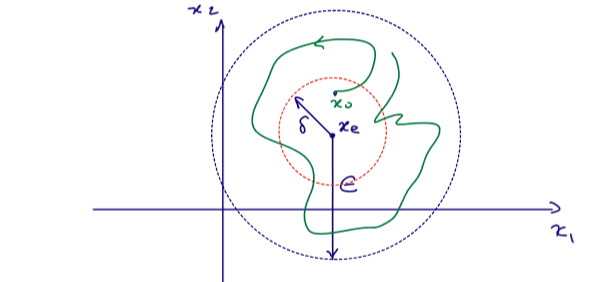
\includegraphics[scale=0.5]{graphics/precise_stability.png}

  \subsubsection{Asymptotic Stability and Exponential Stability}

  The system defined by \(\vect{f}\) is said to be asymptotically stable about \(\vect{x}_{\textrm{eq}}\) iff:

  \(\forall \epsilon > 0,\ \exists \delta > 0 :
  \(\norm{\vect{x}_0 - \vect{x}_{\textrm{eq}}} < \delta \implies \displaystyle
  \lim_{t \to \infty}\norm{\vect{x}(t) - \vect{x}_{\textrm{eq}}} = 0\)

  \textbf{Exponentially Stable}

  A special type of asymptotic stability is exponential stability.

  The system defined by \(\vect{f}\) is said to be exponentially stable about \(\vect{x}_{\textrm{eq}}\) iff:

  \(\forall \epsilon > 0,\ \exists \delta > 0 :
  \(\norm{\vect{x}_0 - \vect{x}_{\textrm{eq}}} < \delta \implies \displaystyle
  \norm{\vect{x}(t) - \vect{x}_{\textrm{eq}}} \le \alpha\norm{\vect{x}_0 - \vect{x}_{\textrm{eq}}}e^{-\beta t}\)

  \subsubsection{Diagram of Stability Types}

  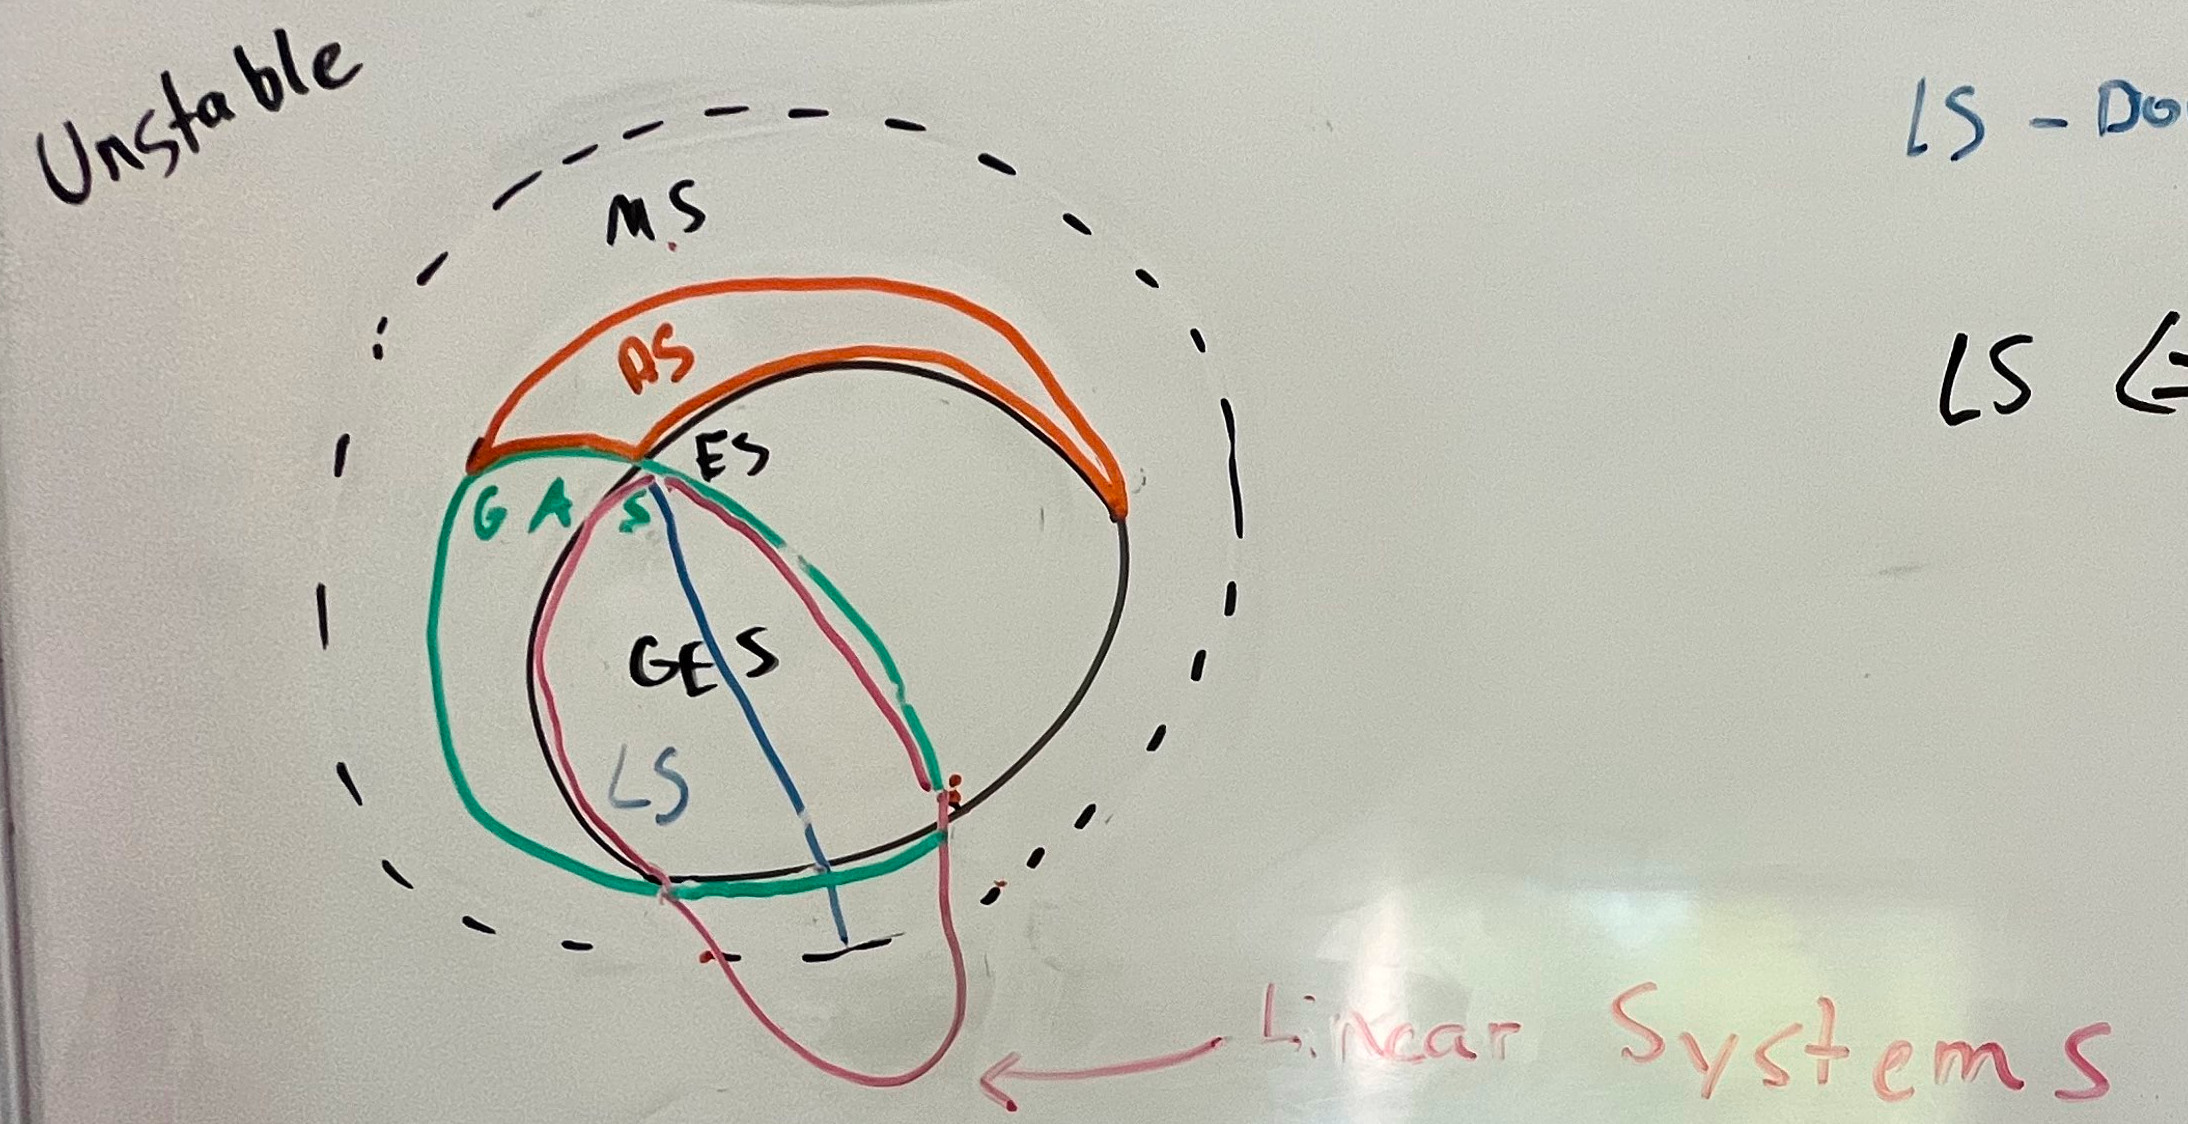
\includegraphics[scale=0.18]{graphics/stability_types.jpg}

  \pagebreak

  \subsection{Example: Equilibria Classification of a Damped Pendulum}

  A damped pendulum with 0 input has the following state space equation:

  \(\begin{bmatrix}
    \dot{\theta} \\
    \ddot{\theta}
  \end{bmatrix} =
  \begin{bmatrix}
    \dot{\theta} \\
    -\frac{g}{L}\sin(\theta) - -b\dot{\theta}
  \end{bmatrix}\)

  We can plot this vector field as a phase diagram in phase space as shown below. Notice that the equilbrium at
  \(\begin{bmatrix} \pi \\ 0 \end{bmatrix}\) is unstable (states are repelled away from it) while the equilibrium
  at \(\begin{bmatrix} 0 \\ 0 \end{bmatrix}\) is stable (states are drawn to it).

  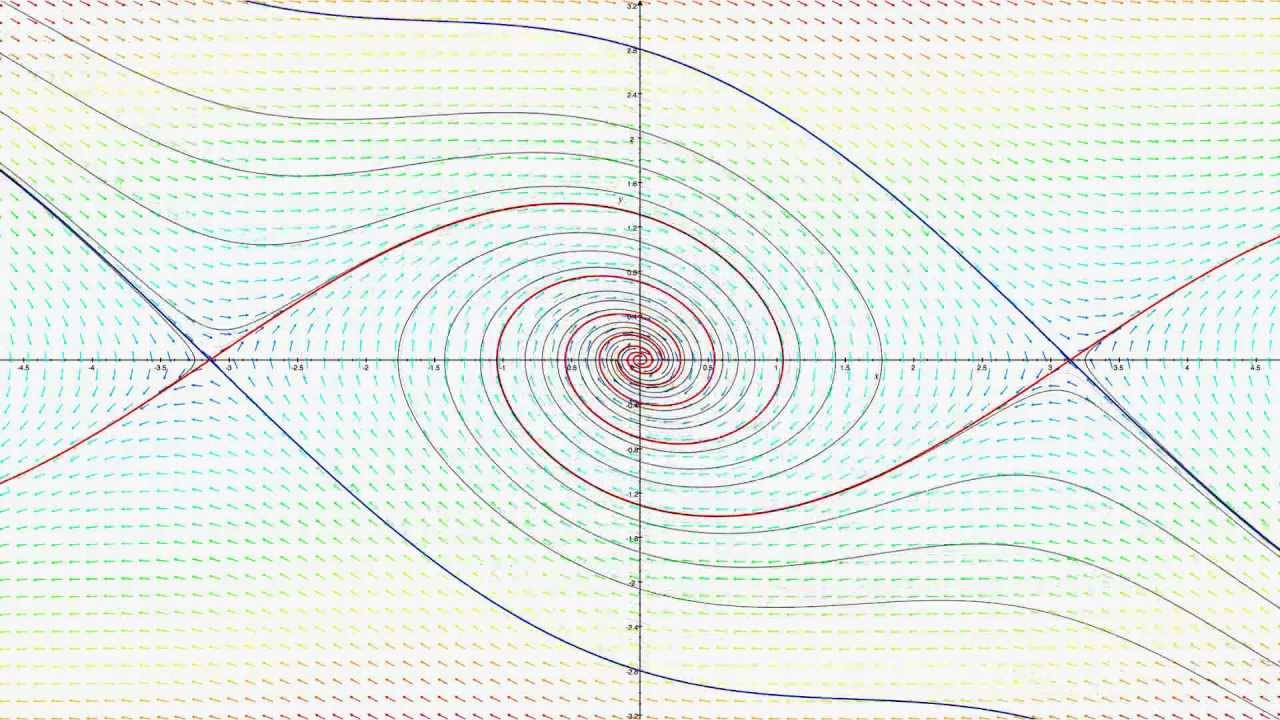
\includegraphics[scale=0.23]{./graphics/pendulum_phase.jpg}

  Now let's analyze this more systematically:

  \(\bkt{\D f(\vect{x})} =
  \begin{bmatrix}
    0 & 1 \\
    -\frac{g}{L}\cos(\theta) & -b
  \end{bmatrix}\)

  But the choice of units is aribtrary. Suppose we chose units such that \(\frac{g}{L} = 1\), \(b = 1\).

  \(\bkt{\D f(\vect{x})} =
  \begin{bmatrix}
    0 & 1 \\
    -\cos(\theta) & -1
  \end{bmatrix}\)

  \vspace{12pt}

  Equilibrum at \(\begin{bmatrix} 0 \\ 0 \end{bmatrix}\).

  \(\bkt{\D f(\vect{x})} =
  \begin{bmatrix}
    0 & 1 \\
    -1 & -1
  \end{bmatrix}\) has eigenvalues \(-\frac{1 + j\sqrt{3}}{2},\, \frac{-1 + j\sqrt{3}}{2}\). Thus we can see that
  the system is asymptotically stable about this equilibrium since both real parts are less than 1.

  \vspace{12pt}

  Equilibrum at \(\begin{bmatrix} \pi \\ 0 \end{bmatrix}\).

  \(\bkt{\D f(\vect{x})} =
  \begin{bmatrix}
    0 & 1 \\
    1 & -1
  \end{bmatrix}\) which has eigenvalues \(\frac{-1 + \sqrt{5}}{2},\, \frac{-1 - \sqrt{5}}{2}\). We can see one eigenvalue
  has real part larger than 1 and thus the system is unstable about this equilibrium.

  \pagebreak

  \subsection{Example: Rotation + Scaling}

  \href{https://www.youtube.com/watch?v=uBlhgAkJBos}{"I'll try spinning, that's a good trick!"}

  A matrix of the form below is called a rotation scaling matrix:

  \(\begin{bmatrix}
    \alpha & -\beta \\
    \beta & \alpha
  \end{bmatrix}\)

  Why? Let \(\theta = \tan^{-1}\prn{\frac{\beta}{\alpha}}\). We now rewrite the matrix as.

  \(\dfrac{1}{\sqrt{\alpha^2 + \beta^2}}
  \begin{bmatrix}
    \cos(\theta) & -\sin(\theta) \\
    \sin(\theta) & \cos(\theta) \\
  \end{bmatrix}\)

  \vspace{12pt}

  Now consider:

  \(\dot{\vect{x}} =
  \begin{bmatrix}
    \alpha & -\beta \\
    \beta & \alpha
  \end{bmatrix}\vect{x}\)

  \begin{flalign*}
    \D\brc{\vect{x}^\T \vect{x}}
    &= 2\vect{x}^\T\dot{\vect{x}}
    &\\
    &= 2\vect{x}^\T
    \begin{bmatrix}
      \alpha & -\beta \\
      \beta & \alpha
    \end{bmatrix}\vect{x}
    &\\
    &=
    2\vect{x}^\T
    \begin{bmatrix}
      \alpha & 0 \\
      0 & \alpha
    \end{bmatrix}\vect{x} +
    \cancelto{\vect{0}}{\vect{x}^\T
    \begin{bmatrix}
      0 & -\beta \\
      \beta & 0
    \end{bmatrix}\vect{x}}
    &\\
    &= 2\alpha\norm{\vect{x}}^2
  \end{flalign*}

  This means \(\norm{\vect{x}(t)}_2 = e^{\alpha t}\norm{\vect{x}_0}_2\) which shows this system is globally exponentially
  stable.

  Intuitively, the antidiagonal terms go to 0 because they represent instantaneous rotation by 90 degrees.
  This corresponds to continuous turning or circular motion (which won't affect the length). You may find
  this property useful when using the Real Jordan Form (see \ref{Real-Jordan-Form}).

  We could've applied this if we analyzed the damped pendulum using the real Jordan Form around its
  equilibrium to show the rotation and scaling around the origin (revealed in the phase plot).

  \pagebreak

  \subsection{The Lyapanov Function}

  \subsubsection{Derivation}

  We saw in the rotation + scaling example that we could use a norm to establish stability properties. We
  now generalize this approach using Lyapanov functions. These are norms on state space.

  \(V(\vect{x}) := \norm{\vect{x}}_{\bm{P}}^2 = \vect{x}^\T\bm{P}\vect{x}\), where \(\bm{P} \in \mathbb{W}_+^n\)
  \begin{flalign*}
    \dot{V}
    &= \D\brc{\vect{x}^\T}\bm{P}\vect{x} + \vect{x}^\T\D\brc{\bm{P}\vect{x}}
    &\\
    &= \dot{\vect{x}}^\T\bm{P}\vect{x} + \vect{x}^\T\bm{P}\dot{\vect{x}}
    &\\
    &= (\bm{A}\vect{x})^\T\bm{P}\vect{x} + \vect{x}^\T\bm{P}\bm{A}\vect{x}
    &\\
    &= \vect{x}^\T\bm{A}^\T\bm{P}\vect{x} + \vect{x}^\T\bm{P}\bm{A}\vect{x}
    &\\
    &= \vect{x}^\T\underbrace{\prn{\bm{A}^\T\bm{P} + \bm{P}\bm{A}}}_{-\bm{Q}}\vect{x}
    &\\
    &= -\vect{x}^\T\bm{Q}\vect{x}
  \end{flalign*}
  Thus \(\bm{Q} \succ 0 \implies \dot{V} < 0\).

  Some authors define the Lyapanov operator as \(\bm{L}_{\bm{A}}(\bm{P}) = \bm{A}^\T\bm{P} + \bm{P}\bm{A}\)

  \subsubsection{Application to Establishing GES of Asymptotically Stable LTI Systems}

  Recall a norm with respect to a matrix is bounded by its eigenvalues times the 2 norm.

  \(-\lambda_{\textrm{max}}(\bm{W}_1)\norm{\vect{x}}^2 \le
  \dot{V}(\vect{x}) \le -\lambda_{\textrm{min}}(\bm{W}_1)\norm{\vect{x}}^2\)

  \(\implies \dot{V} \le -\lambda_{\textrm{min}}(\bm{W}_1)\norm{\vect{x}}^2\)

  \vspace{12pt}

  Let's replace \(\norm{\vect{x}}^2\) as well. We also know:

  \(\lambda_{\textrm{min}}(\bm{P})\norm{\vect{x}}^2 \le V(\vect{x}) \le \lambda_{\textrm{max}}(\bm{P})\norm{\vect{x}}^2\)

  \(\lambda_{\textrm{max}}(\bm{P})\norm{\vect{x}}^2 \le -V(\vect{x}) \le \lambda_{\textrm{min}}(\bm{P})\norm{\vect{x}}^2\)

  \(\lambda_{\textrm{max}}(\bm{P})\norm{\vect{x}}^2 \le -V(\vect{x})\)

  \(\norm{\vect{x}}^2 \le -\dfrac{1}{\lambda_{\textrm{max}}(\bm{P})} V(\vect{x})\)

  \vspace{12pt}

  Substuting this back in we have:

  \(\dot{V} \le -\underbrace{\dfrac{\lambda_{\textrm{min}}(\bm{Q})}{\lambda_{\textrm{max}}(\bm{P})}}_{2\alpha}V(\vect{x})\)

  \(\dot{V} \le \alpha V(\vect{x})\)

  \(\implies V(\vect{x}) \le e^{-2\alpha t}V_0\)

  So if \(\dfrac{\lambda_{\textrm{min}}(\bm{Q})}{\lambda_{\textrm{max}}(\bm{P})} > 0\), the Lyapanov function decays
  exponentially.

  \pagebreak

  Plugging this back into the inequality we have:

  \(\lambda_{\textrm{min}}(\bm{P})\norm{\vect{x}}^2 \le V(\vect{x}) \le e^{-2\alpha t}V_0\)

  \(\lambda_{\textrm{min}}(\bm{P})\norm{\vect{x}}^2 \le e^{-2\alpha t}V_0\)

  \(\norm{\vect{x}}^2 \le e^{-2\alpha t}\dfrac{V(\vect{x}_0)}{\lambda_{\textrm{min}}(\bm{P})}\)

  \(\norm{\vect{x}} \le \sqrt{e^{-2\alpha t}\dfrac{V(\vect{x}_0)}{\lambda_{\textrm{min}}(\bm{P})}}\)

  \(\norm{\vect{x}} \le e^{-\alpha t}\sqrt{\dfrac{V(\vect{x}_0)}{\lambda_{\textrm{min}}(\bm{P})}}\)

  The 2-norm is decreasing, bounded by \(e^{-\alpha t}\). So we can now see that all asymptotically
  stable LTI systems are globally exponentially stable.

  \subsubsection{Solving for P Given A and Q}

  We'll see how we different choices of \(\bm{Q}\) can lead to interesting types of Lyapanov functions
  which have important physical interpretations. But that's getting ahead of things. For now, we
  want to know when given \(\bm{A}\) and \(\bm{Q}\) if we can find a \(\bm{P}\) such that:

  \(\bm{A}^\T\bm{P} + \bm{P}\bm{A} = -\bm{Q}\)

  In fact the above equation is known as a linear matrix equation (LME). In particular, these
  types of LMEs are common in control theory and are called
  \href{https://www.wikiwand.com/en/Sylvester_equation}{Sylvester equations}. In general,
  there are efficient numerical methods which can solve these types of equations in \(\mathcal{O}(n^3)\) operations.

  \vspace{12pt}

  An analytic solution is given through use of \href{https://www.wikiwand.com/en/Vectorization_(mathematics)}{vectorization}
  and the \href{https://www.wikiwand.com/en/Kronecker_product#Matrix_equations}{Kronecker Product}.


  \((\bm{A} \kronsum \bm{I}_n)\textrm{vec}(\bm{P}) = -\textrm{vec}(\bm{Q})\)

  So the solution is unique when \(\bm{A} \kronsum \bm{I}_n\) is invertible.

  \(\bm{A} \kronsum \bm{I}_n\) has eigenvalues \(\lambda_i + \lambda_j\), \(\lambda_i, \lambda_j \in \spec{\bm{A}}\), so
  we have unique solutions when \(\lambda_i + \lambda_j \neq 0\)

  \subsubsection{Lyapanov Function When A is Hurwitz}

  Notice when solving the Sylvester equation for \(\bm{P}\), it is sufficient for \(\bm{A}\) to be Hurwitz.
  Start by noticing that the Lyapanov operator is a product rule. The idea behind the
  subsitution is very similar to the use of an integrating factor when solving first order
  linear ODEs.

  \(\bm{L}_{\bm{A}}(\bm{P}) = \bm{A}^\T\bm{P} + \bm{P}\bm{A}\)

  Choose \(\displaystyle \bm{P} = \int_0^\infty e^{\bm{A}^\T t} \bm{Q} e^{\bm{A} t}\, dt \)

  \pagebreak

  Subsituting back in to the Lyapanov operator, we have:
  \begin{flalign*}
    \bm{L}_{\bm{A}}\prn{\int_0^\infty e^{\bm{A}^\T t} \bm{Q} e^{\bm{A} t}\, dt}
    &=
    \bm{A}^\T \prn{\int_0^\infty e^{\bm{A}^\T t} \bm{Q} e^{\bm{A} t}\, dt} +
    \prn{\int_0^\infty e^{\bm{A}^\T t} \bm{Q} e^{\bm{A} t}\, dt}\bm{A}
    &\\
    &=
    \int_0^\infty \bm{A}^{\T} e^{\bm{A}^\T t} \bm{Q} e^{\bm{A} t}
     + e^{\bm{A}^\T t} \bm{Q} e^{\bm{A} t}\bm{A}\, dt
    &\\
    &=
    \int_0^\infty \dfrac{d}{dt} \bkt{e^{\bm{A}^\T t} \bm{Q} e^{\bm{A} t}}\, dt
    &\\
    &= \eval{e^{\bm{A}^\T t} \bm{Q} e^{\bm{A} t}}_0^\infty
    &\\
    &= -\bm{Q}
  \end{flalign*}

  \textbf{Interpretation of the Lyapanov Function for Hurwitz Matricies}

  Let's plug in a constant vector to the Lyapanov equation and see what happpens.
  \begin{flalign*}
    V(\vect{x}_0)
    &= \vect{x}_0^{\T}\prn{\int_0^\infty e^{\bm{A}^\T t} \bm{Q} e^{\bm{A} t}\, dt}\vect{x}_0
    &\\
    &= \int_0^\infty \vect{x}_0^{\T}e^{\bm{A}^\T t} \bm{Q} e^{\bm{A} t}\vect{x}_0\, dt
    &\\
    &= \int_0^\infty \norm{\vect{x}(t)}^2_{\bm{Q}}\, dt
  \end{flalign*}
  Thus we can see this as a form of cost to move from state \(\vect{x}_0\) to \(\vect{x}_{\textrm{eq}}\). Another
  view is this characterizes the work done passively by the system in moving from \(\vect{x}_0\)
  to \(\vect{x}_{\textrm{eq}}\). Different choices of \(\bm{Q}\), of course, will yield different values for
  how much "work" or "cost" there is.

  \pagebreak

  \subsection{Controllablity}

  \subsubsection{Definitions}

  \textbf{Definition}: Set of States Reachable in in \(t\) time or \(\nu\) epochs

  The reachable subspace of a LTI system given by \(\bm{A}, \bm{B}, \bm{C}, \bm{D}\)

  Continuous time:

  \(R_t := \displaystyle
  \brc{\left.\int_0^t e^{(t - \tau)\bm{A}}\bm{B}\vect{u}(\tau)\,d\tau\ \right\vert\ \vect{u} : [0, t] \to \mathbb{R}^m}\)

  Discrete time:

  \(R_\nu := \displaystyle
  \brc{\left.\sum_{k = 0}^{\nu - 1} \bm{A}^{\nu - k - 1}\bm{B}\vect{u}[k]\ \right\vert\ \vect{u} : [0\,..\,t] \to \mathbb{R}^m}\)

  Notice that \(t_2 > t_1 \implies \mathcal{R}_{t_2} \subseteq \mathcal{R}_{t_1} \)

  Intuitively this makes sense. We can reach more states given more time.

  \vspace{12pt}

  \textbf{Definition}: Reachable Subspace

  \(R := \displaystyle \bigcup_{t \ge 0} R_t\)

  This is the set of all states reachable given some input and unlimited time. We'll see
  why we know this is a subspace in a bit.

  \vspace{12pt}

  \textbf{Definition}: Controllable

  A system is controllabe iff \(R = \mathbb{R}^m\).

  That is, any state is reachable given enough time.

  \subsubsection{Discrete Time Controllability}

  In a pratical sense, it would be impossible to search over all possible inputs over infinite time to see
  if all states are truly reachable. We'll need to develop a better way of analyzing controllability.

  Let's start by recalling in discrete time:

  \(\vect{x}[1] = \bm{A}\vect{x}[0] + \bm{B}\vect{u}[0]\)
  \begin{flalign*}
    \vect{x}[2]
    &= \bm{A}\vect{x}[1] + \bm{B}\vect{u}[0]
    &\\
    &=
    \bm{A}(\bm{A}\vect{x}[0] + \bm{B}\vect{u}[0]) +
    \bm{B}\vect{u}[1]
    &\\
    &= \bm{A}^2\vect{x}[0] + \bm{A}\bm{B}\vect{u}[0] + \bm{B}\vect{u}[1]
  \end{flalign*}
  Continuing on inductively we have:

  \(\vect{x}[\nu] = \bm{A}^{\nu}\vect{x}[0] +  \displaystyle
  \sum_{k = 0}^{\nu - 1} \bm{A}^{\nu - k - 1}\bm{B}\vect{u}[k]\)

  \pagebreak

  Define:

  \(\mathcal{C}_{\nu} := \begin{bmatrix} \bm{B} & \bm{AB} & \dots & \bm{A}^{\nu - 1}\bm{B}\end{bmatrix}\)

  \vspace{12pt}

  We can now write:

  \(\vect{x}[\nu] = \bm{A}^nx[\nu] +
  \mathcal{C}_{\nu}
  \begin{bmatrix} \vect{u}[\nu - 1] \\ \vdots \\ \vect{u}[0] \end{bmatrix}\)

  \vspace{12pt}

  We can now see the set of states reachable in \(\nu\) epochs is \(R_{\nu} = \img{\mathcal{C}_{\nu}}\).
  How big can \(\mathcal{R}_v\) get? Recall the Caley-Hamilton theorem.

  \(\charc{\bm{A}}(\bm{A}) = [0]\). Thus we can see that a linear combination of \(\bm{A}, \dots, \bm{A}^n\) are
  not linearly independent. Thus the biggest the rank can get is \(n\). This means that
  an input function defined for n epochs will let you access the entire reachable subspace.

  \vspace{12pt}

  \textbf{Definition}: Controllability Matrix

  \(\mathcal{C} := \begin{bmatrix} \bm{B} & \bm{AB} & \dots & \bm{A}^{n - 1}\bm{B}\end{bmatrix}\),
  \(\mathcal{C} \in \mathbb{R}^{n \times np}\)

  The system is controllable iff \(\rank(\mathcal{C}) = n\)

  \pagebreak

  \subsubsection{Continuous Time Controllability}

  It turns out that the controllability matrix is the same in continuous time as in discrete time.
  Let's derive this.

  \textbf{Lemma}:

  \(\bm{A}^k\) is linearly dependent with \(\bm{A}, \dots, \bm{A}^{n - 1}\ \ \forall k \ge n\)
  \begin{flalign*}
    e^{\bm{A}t}
    &:= \sum_{k = 0}^{\infty} \dfrac{(\bm{A}t)^k}{k!}
    &\\
    &= \sum_{k = 0}^{n - 1} \dfrac{(\bm{A}t)^k}{k!} +
    \sum_{k = n}^{\infty} \dfrac{(\bm{A}t)^k}{k!}
    &\\
    &= \sum_{k = 0}^{n - 1} c_k(t) \bm{A}^k
  \end{flalign*}
  \begin{flalign*}
    \vect{x}(t)
    &= e^{\bm{A}t}\vect{x}_0 + \int_{0}^{t} e^{\bm{A}\tau}\bm{B}\vect{u}(t - \tau)\, d\tau
    &\\
    &= e^{\bm{A}t}\vect{x}_0 + \int_{0}^{t} \prn{\sum_{k = 0}^{n} c_k(\tau) \bm{A}^k}\bm{B}\vect{u}(t - \tau)\, d\tau
    &\\
    &= e^{\bm{A}t}\vect{x}_0 +
    \sum_{k = 0}^{n - 1}\bm{A}^k\bm{B}
    \int_{0}^{t} c_k(\tau) \vect{u}(t - \tau)\, d\tau
    &\\
    &= e^{\bm{A}t}\vect{x}_0 +
    \underbrace{\begin{bmatrix} \bm{B} & \bm{AB} & \dots & \bm{A}^{n - 1}\bm{B}\end{bmatrix}}_{\mathcal{C}}
    \begin{bmatrix}
      \displaystyle \int_{0}^{t} c_1(\tau) \vect{u}(t - \tau)\, d\tau  \\
      \vdots \\
      \displaystyle \int_{0}^{t} c_{n - 1}(\tau) \vect{u}(t - \tau)\, d\tau  \\
    \end{bmatrix}
   &\\
    &= e^{\bm{A}t}\vect{x}_0 +
    \mathcal{C}
    \begin{bmatrix}
      \displaystyle \int_{0}^{t} c_1(\tau) \vect{u}(t - \tau)\, d\tau  \\
      \vdots \\
      \displaystyle \int_{0}^{t} c_{n - 1}(\tau) \vect{u}(t - \tau)\, d\tau  \\
    \end{bmatrix}
  \end{flalign*}

  We assume that the functions \(c_k(t) \neq 0\ \forall t\)

  Notice that reachability in continuous time only depends on \(\mathcal{C}\). Given a large enough
  input vector, we can reach any state that is in \(\img{\mathcal{C}}\), so once again, the system
  is controllable iff \(\rank(\bm{C}) = n\)

  \pagebreak

  There is a simpler way of deriving the controllability matrix shown below.

  \(\dot{\vect{x}} = \bm{A}\vect{x} + \bm{B}\vect{u}\)

  \(\ddot{\vect{x}} = \bm{A}^2\vect{x} + \bm{A}\bm{B}\vect{u} + \bm{B}\dot{\vect{u}}\)

  Continuing inductively:
  \begin{flalign*}
    \vect{x}^{(\nu)}
    &= \bm{A}^{\nu}\vect{x} + \sum_{k = 0}^{\nu - 1} \bm{A}^{\nu - k - 1}\bm{B} \vect{u}^{(k)}
    &\\
    &= \bm{A}^{\nu}\vect{x} +
    \begin{bmatrix} \bm{B} & \bm{AB} & \dots & \bm{A}^{\nu - 1}\bm{B} \end{bmatrix}
    \begin{bmatrix}
      \vect{u}^{(n)} \\
      \vdots \\
      \vect{u}
    \end{bmatrix}
    &\\
    &= \bm{A}^{\nu}\vect{x} +
    \mathcal{C}
    \begin{bmatrix}
      \vect{u}^{(n)} \\
      \vdots \\
      \vect{u}
    \end{bmatrix}
  \end{flalign*}
  Thus we have:

  \(\mathcal{C}
   \begin{bmatrix}
      \vect{u}^{(n)} \\
      \vdots \\
      \vect{u}
    \end{bmatrix}
  =
  \vect{x}^{n} - \bm{A}^{n}\vect{x}\)

  If \(\mathcal{C}\) is full rank (that is, the system is controllable), we can make the right hand side
  (the state derivatives of power \(n\)) anything we want. This is analogous to being able to
  fully specify the state with an input.

  \pagebreak

  \subsubsection{Controllability Indicies}

  Recall that \(\bm{B} \in \mathbb{R}^{n \times p}\) maps the p inputs to the n states of the system.

  Let's express \(\bm{B} = \begin{bmatrix} \vect{b}_1 & \cdots & \vect{b}_{p}\end{bmatrix}\)

  Now we can rewrite the controllability matrix as:
  \begin{flalign*}
    \mathcal{C}
    &= \begin{bmatrix} \bm{B} & \bm{AB} & \cdots & \bm{A}^{n - 1}\bm{B} \end{bmatrix}
    &\\
    &= \begin{bmatrix}
      \ \ \vect{b}_1 & \cdots & \vect{b}_p &
      \Big\vert & \bm{A}\vect{b}_1 & \cdots & \bm{A}\vect{b}_p & \Big\vert & \cdots & \Big\vert &
      \bm{A}^{n - 1}\vect{b}_1 & \cdots & \bm{A}^{n - 1}\vect{b}_p \ \
    \end{bmatrix}
  \end{flalign*}

  \textbf{Lemma}:

  If \(\bm{A}^{\mu}\vect{b}_{i}\) is linearly dependent on left hand side columns, then so is
  \(\bm{A}^{\mu + 1}\vect{b}_i\).

  \textbf{Proof}:

  Suppose \(\bm{A}^{\mu}\vect{b}_{m}\) is linearly dependent on left hand side columns. That means
  we can write:

  \(\bm{A}^{\mu}\vect{b}_m = \displaystyle
  \sum_{k = 0}^{\mu - 1}\sum_{i = 0}^{p} c_{ik}\bm{A}^k\vect{b}_i\)
  \begin{flalign*}
    \bm{A}^{\nu + 1}\vect{b}_m
    &= \bm{A}\sum_{k = 0}^{\mu}\sum_{i = 0}^{p} c_{ik}\bm{A}^k\vect{b}_i
    &\\
    &= \sum_{k = 0}^{\mu - 1}\sum_{i = 0}^{p} c_{ik}\bm{A}^{k + 1}\vect{b}_i
    &\\
    &= \sum_{k = 1}^{\mu}\sum_{i = 0}^{p} c_{ik}\bm{A}^{k}\vect{b}_i
  \end{flalign*}
  ---

  This lemma means we can group columns of \(\bm{A}^k\bm{b}_m\) like so:

  \(\underbrace{\vect{b}_i,\ \bm{A}\vect{b}_i,\ \dots,\ \bm{A}^{\mu - 1}\vect{b}_mi\ }_{\textrm{Linearly independent}} \big\vert\
  \underbrace{\bm{A}^{\mu}\vect{b}_i,\ \dots,\ \bm{A}^{n - 1}\vect{b}_i}_{\textrm{Linearly dependent on LHS}}\)

  So each \(\vect{b}_i\) is associated with \(\mu_i\) linearly independent columns of \(\mathcal{C}\). These
  \(\mu_i\) are called controllability indicies.

  It follows that \(\rank(\mathcal{C}) = \displaystyle \sum_{m = 1}^p \mu_m\)

  \textbf{Definition: Controllability Index}

  \(\mu := \displaystyle \max \brc{\mu_m}_{m = 1}^p\)

  \pagebreak

  \textbf{Theorem: Redundant Control Modes}

  The controllability index shows we don't need all columns of the controllability matrix. Now we show this.
  First let's order the controllability from least to greatest so that \(\mu_p = \mu\)

  \(\mathcal{C} =
  \begin{bmatrix}
    \bm{B} &
    \bm{AB} & \cdots &
    \bm{A}^{\mu_1}\bm{B} & \cdots &
    \bm{A}^{\mu}\bm{B} & \cdots &
    \bm{A}^{n - 1}\bm{B}
  \end{bmatrix}\)

  \(\bm{A}^{\mu}\bm{B}\) contains all the linearly independent columns of \(\bm{A}^k\bm{b}_m\) implied by
  all the other controllability indices (since they require powers of \(\bm{A}\) less than \(\mu\)). This means:

  \(\rank\prn{\begin{bmatrix} \bm{B} & \bm{AB} & \cdots & \bm{A}^\mu\bm{B}\end{bmatrix}} = \rank(\mathcal{C})\).

  ---

  \textbf{Theorem: Controllability Index Bounds}

  We'll start by assuming \(\rank(\mathcal{C}) = n\).

  \vspace{12pt}

  Lower bound:

  The smallest possible \(\mu\) happens when all the \(\mu_m\) are the same. In which case:

  \(\displaystyle \sum_{i = 0}^p \mu_m = p\mu_{\textrm{min}} = n\)

  \(\implies \mu_{\textrm{min}} = \frac{n}{p}\)

  \vspace{12pt}

  Upper bound 1:

  If all the \(\mu_m\) are 1 except \(\mu\), then we have

  \(\displaystyle \sum_{i = 0}^p \mu_m = \mu_{\textrm{max}} + p - 1 = n\)

  \(\implies \mu_{\textrm{max}} = n - p + 1\)

  \vspace{12pt}

  Upper bound 2:

  We can also generate a tigher upper bound by using the on the minimal polynomial.

  Let \(\deg{\minpoly{\bm{A}}(\lambda)} = \tilde{n}\).

  \(\minpoly{\bm{A}}(\bm{A}) = \displaystyle
  \bm{A}^{\tilde{n}} + \sum_{k = 0}^{\tilde{n} - 1} c_k\bm{A}^k = [0]\)

  \(\implies \bm{A}^{\tilde{n}} = \displaystyle \sum_{k = 0}^{\tilde{n} - 1} c_k\bm{A}^k\) (the \(c_k\) are arbitrary so I can
  drop the sign from the subtraction)

  \vspace{12pt}

  Thus we have the bounds:

  \(\frac{n}{p} \le \mu \le \min\brc{n - p + 1,\ \deg{\minpoly{\bm{A}}}(\lambda)}\)

  \pagebreak


  \textbf{Corollary: Reduced Controllability}

  We can use \(\mu\) to reduce the number of columns we need to check for controllability. The maximum bound using
  the minimal polynial can be somewhat hard to find, so we'll estimate \(\mu \le n - p + 1\)

  Thus the system is controllable iff:

  \(\rank\prn{\begin{bmatrix} \bm{B} & \bm{AB} & \cdots & \bm{A}^{n - p}\bm{B}\end{bmatrix}} = n\).

  \subsubsection{Controllability is Coordinate Independent}

  Intuitively, the choice of units we use for our state space should not affect the controllability. Indeed
  it doesn't. We now prove this. Suppose we represent our state space with new basis \(\mathcal{B}\). Recall from
  the Section \ref{state-space-coord} discussion on state space coordinate systems:

  \(\bm{A} = \bm{P}\bm{A}_{\mathcal{B}}\bm{P}^{-1}\), \(\bm{B} = \bm{P}\bm{B}_{\mathcal{B}}\)
  \begin{flalign*}
    \mathcal{C}
    &=
    \begin{bmatrix}
      \bm{P}\bm{B}_{\mathcal{B}} &
      (\bm{P}\bm{A}_{\mathcal{B}}\cancel{\bm{P}^{-1}})(\cancel{\bm{P}}\bm{B}_{\mathcal{B}}) & \dots
      (\bm{P}\bm{A}^n_{\mathcal{B}}\cancel{\bm{P}^{-1}})(\cancel{\bm{P}}\bm{B}_{\mathcal{B}})
    \end{bmatrix}
    &\\
    &=
    \begin{bmatrix}
      \bm{P}\bm{B}_{\mathcal{B}} &
      \bm{P}\bm{A}_{\mathcal{B}}\bm{B}_{\mathcal{B}} & \dots &
      \bm{P}\bm{A}^n_{\mathcal{B}}\bm{B}_{\mathcal{B}}
    \end{bmatrix}
    &\\
    &=
    \bm{P}
    \underbrace{\begin{bmatrix}
      \bm{B}_{\mathcal{B}} &
      \bm{A}_{\mathcal{B}}\bm{B}_{\mathcal{B}} & \dots &
      \bm{A}^n_{\mathcal{B}}\bm{B}_{\mathcal{B}}
    \end{bmatrix}}_{\mathcal{C}_{\mathcal{B}}}
    &\\
    &= \bm{P}\mathcal{C}_{\mathcal{B}}
  \end{flalign*}
  But since \(\bm{P}\) is a change of basis matrix, it must be invertible. Invertible matrices
  can expressed as a sequence of elementary row operations
  \(\bm{P} = \displaystyle \prod_{k = 0}^{\nu} \bm{E}_k\) where \(\bm{E}_k\).

  Since row operations do not change rank we have:

  \(\rank(\mathcal{C}) = \rank(\bm{P}\mathcal{C}_{\mathcal{B}}) = \rank(\mathcal{C}_{\mathcal{B}})\)

  \pagebreak

  \subsubsection{The Controllable and Uncontrollable Subspace}

  An invariant subspace is a subspace \((V, \mathbb{F}) : \bm{A}V = V\)

  Eigenspaces (span of eigenvectors) are clearly invariant subspaces and so is \(\brc{\vect{0}}\) and \(\mathbb{R}^n\)
  What other subspaces might be invariant? Well consider an block upper triangular matrix.

  \(\bm{A} =
  \begin{bmatrix}
    \bm{A}_{11} & \bm{A}_{12} \\
    0 & \bm{A}_{22}
  \end{bmatrix}\) where \(\bm{A}_{11} \in \mathbb{R}^{r \times r}\)

  Clearly \(V = \brc{\left.\begin{bmatrix} \vect{v}_r \\ 0 \end{bmatrix} \right\vert \vect{z} \in \mathbb{R}^r}\)
  is an invariant subspace.

  \textbf{Theorem:} The Controllable Subspace is A-invariant
  \begin{flalign*}
    \bm{A}\begin{bmatrix} \bm{B} & \bm{AB} & \dots & \bm{A}^{n - 1}\bm{B} \end{bmatrix}\vect{v}_k
    &= \bm{A} \sum_{k = 0}^{n - 1} \bm{A}^{n - k - 1}\bm{B}\vect{v}_k
    &\\
    &= \sum_{k = 0}^{n - 1} \bm{A}^{n - k}\bm{B}\vect{v}_k
    &\\
    &= \bm{A}^n\bm{B}\vect{v}_{0} + \sum_{k = 1}^{n - 1} \bm{A}^{n - k}\bm{B}\vect{v}_k
    &\\
    &= \sum_{k = 1}^{n - 1} c_k\bm{A}^{n - k}\bm{B}\vect{v}_{0} +
    \sum_{k = 1}^{n - 1} \bm{A}^{n - k}\bm{B}\vect{v}_k
    &\\
    &= \begin{bmatrix} \bm{B} & \bm{AB} & \dots & \bm{A}^{n - 1}\bm{B} \end{bmatrix}
    \begin{bmatrix}
      0 \\
      \vect{v}_1 + c_1\vect{v}_0 \\
      \vdots \\
      \vect{v}_{n - 1} + c_{n - 1}\vect{v}_0 \\
    \end{bmatrix}
  \end{flalign*}
  \(\implies \bm{A}\img{\mathcal{C}} = \img{\mathcal{C}}\)

  ---

  We can characterize an invariant subspace with a matrix.

  Let \((V, \mathbb{F}) \subset \mathbb{R}^{n \times k}\) be
  an invariant subspace spanned by \(\vect{v}_1, \dots, \vect{v}_k\)

  Define:

  \(\bm{M} = \begin{bmatrix} \vect{v}_1 & \cdots & \vect{v}_k \end{bmatrix}\)

  Notice that:

  \(\bm{A}\vect{v}_1 = \displaystyle \sum_{k = 1}^k x_{1, k}\vect{v}_k\)

  \(\bm{A}\vect{v}_2 = \displaystyle \sum_{k = 1}^k x_{2, k}\vect{v}_k\)

  \(x_{i, k}\) forms the entries of a matrix \(\bm{X}\)

  \(\bm{A}\bm{M} = \bm{M}
  \begin{bmatrix}
    x_{1, 1}  & \cdots & x_{1,k}  \\
    \vdots & & \vdots \\
    x_{k, 1}  & \cdots & x_{k,k}  \\
  \end{bmatrix}\)

  So we have:

  \(\bm{A}\bm{M} = \bm{M}\bm{X}\)

  So \(\img{\bm{M}}\) is A-invariant \(\iff \exists \bm{X} : \bm{A}\bm{M} = \bm{M}\bm{X}\)

  Which is a Sylvester equation. We know this has solutions when \(\bm{A}\) and \(\bm{M}\)
  don't share eigenvalues.

  Now consider \(\tilde{\bm{M}} \in \mathbb{R}^{n \times (n - k)}\).
  \begin{flalign*}
    \bm{A}\begin{bmatrix} \bm{M} & \tilde{\bm{M}}\end{bmatrix}
    &= \begin{bmatrix} \bm{A}\bm{M} & \bm{A}\tilde{\bm{M}}\end{bmatrix}
    &\\
    &= \begin{bmatrix} \bm{M} & \tilde{\bm{M}}\end{bmatrix}
    \begin{bmatrix}
      \bm{X} & \bm{A}_{12} \\
      0 & \bm{A}_{22}
    \end{bmatrix}
  \end{flalign*}
  where \(\begin{bmatrix} \bm{A}_{12} \\ \bm{A}_{22} \end{bmatrix} =
  \begin{bmatrix} \bm{M} & \tilde{\bm{M}} \end{bmatrix}^{-1}\bm{A}\tilde{\bm{M}}\)

  So if we have \(\bm{P} = \begin{bmatrix} \bm{M} & \tilde{\bm{M}}\end{bmatrix}\)

  \(\bm{P}^{-1}\bm{A}\bm{P} =
  \begin{bmatrix}
    \bm{A}_{11} & \bm{A}_{12} \\
    0 & \bm{A}_{22}
  \end{bmatrix}\)

  \vspace{12pt}

  So as long as we select \(\tilde{\bm{M}}\) so that \(\bm{P}\) is invertible we can reveal
  the controllable subspace.

  \(\bm{P}^{-1}\bm{A}\bm{P} =
  \begin{bmatrix}
    \bm{A}_{c} & \bm{A}_{12} \\
    0 & \bm{A}_{22}
  \end{bmatrix}\),
  \(\bm{P}^{-1}\bm{B} = \begin{bmatrix} \bm{B}_c \\ 0 \end{bmatrix}\)

  \(\bm{P}^{-1}\mathcal{C} =
  \begin{bmatrix}
    \bm{B}_c  & \bm{B}_c\bm{A}_{c} & \cdots & \bm{A}_{c}^{n - 1}\bm{B}_c \\
    0 & 0 & \cdots & 0
  \end{bmatrix}\)

  In general we can select the first \(n\) linearly independent columns of \(\mathcal{C}\) and
  then any \(n - k\) columns of \(\mathcal{C}\) so that \(\bm{M}\) is invertible.

  \pagebreak

  \subsubsection{Impulse Inputs}
  Recall in continuous time, we can reach any state given a large enough input.
  The "largest" input vector we could provide are impulse inputs and inputs that are
  distriubtional derivatives of the impulse (in general you don't need to know what this
  means but that it behaves like a derivative to the Laplace transform).

  \textbf{Lemma}:

  Recall that \(f(x) = \dfrac{1}{1 - x} = \displaystyle \sum_{k = 0}^\infty x^n\)

  \((s\bm{I}_n - \bm{A})^{-1} = \displaystyle \sum_{k = 0}^\infty s^{-k}\bm{A}^k\)

  ---

  \vspace{12pt}

  Now for a single input system choose:

  Consider \(u(t) = \vect{v}\delta^{(k)}(t)\)

  \(U(s) = \vect{v}s^\nu\)
  \begin{flalign*}
    \bm{X}(s)
    &= (s\bm{I}_n - \bm{A})^{-1}\bm{B}\bm{U}(s)
    &\\
    &= (s\bm{I}_n - \bm{A})^{-1}\bm{B}\vect{v}s^{\nu}
    &\\
    &= \prn{\sum_{k = 0}^{\infty} s^{-k}\bm{A}^k} \bm{B}\vect{v}s^{\nu}
    &\\
    &= \prn{\sum_{k = 0}^{\infty} s^{\nu - k}\bm{A}^k}\bm{B}\vect{v}
    &\\
    &= \prn{\underbrace{\sum_{k = 0}^{\nu - 1} s^{\nu - k}\bm{A}^k}_{\textrm{Impulse terms}} +
    \sum_{k = \nu}^{\infty} s^{\nu - k}\bm{A}^k}\bm{B}\vect{v}
  \end{flalign*}
  \(x(t) = \displaystyle \textrm{Impulse terms} + \sum_{k = \nu}^\infty \dfrac{t^k}{k!}\bm{A}^k\bm{B}\vect{v}\)

  So we have:

  \(x(0^+) = \bm{A}^k\bm{B}\vect{v}\)

  Now choose \(u(t) = \displaystyle \sum_{k = 0}^{n - 1}\vect{v}_k\delta^{(k)}(t)\)

  \pagebreak

  By linearity we'll have:

  \(x(0^+) = \displaystyle \sum_{k = 0}^{n - 1} c_k\bm{A}^k\bm{B}
  = \underbrace{\begin{bmatrix} \bm{B} & \bm{AB} & \dots & \bm{A}^{n - 1}\bm{B}\end{bmatrix}}_{\mathcal{C}}
  \begin{bmatrix}
    \vect{v}_0 \\
    \vdots \\
    \vect{v}_{n - 1}
  \end{bmatrix} =
  \mathcal{C}
  \begin{bmatrix}
    \vect{v}_0 \\
    \vdots \\
    \vect{v}_{n - 1}
  \end{bmatrix}\)

  \vspace{12pt}

  Thus \(\vect{x}(0^+)\) can be made to be any element of \(\img{\mathcal{C}}\). Intuitively,
  given infinite inputs, we can steer the system state to be anything in the
  reachable subspace instantaneously.

  \subsection{Least Norm Input}

  Often we want to get to a reachable state while minimizing the work spent to get there. To do this we minimize:

  \(\displaystyle \int_0^t \norm{\vect{u}(\tau)}^2\,d\tau\)

  \vspace{12pt}

  \textbf{Discrete Time}

  Let's start by discretizing \(\bm{u}\). Let it be piecewise constant
  on \(\vect{u}\) with duration \(h = \frac{t_f}{N}\).

  \(u(\tau) = u_d[k]\), \(\ kh \le \tau < (k + 1)h\) where \(k \in [0\,..\,N - 1]\)

  Let \(\bm{A}_d = e^{\bm{A}h}\), \(\bm{B}_d = \displaystyle \prn{\int_{0}^h e^{\bm{A}\tau}\,d\tau}\bm{B}\)

  \(\vect{x}_{\textrm{dst}} =
  \begin{bmatrix} \bm{B}_d & \bm{A}_d\bm{B}_d & \dots & \bm{A}_d^{N - 1}\bm{B}_d\end{bmatrix}
  \begin{bmatrix} \vect{u}_d[N - 1] \\ \vdots \\ \vect{u}_d[0] \end{bmatrix}\)
  \begin{flalign*}
    \begin{bmatrix} \vect{u}_d[N - 1] \\ \vdots \\ \vect{u}_d[0] \end{bmatrix}_{\textrm{ln}}
    &= \begin{bmatrix} \bm{B}_d & \bm{A}_d\bm{B}_d & \dots & \bm{A}_d^{N - 1}\bm{B}_d\end{bmatrix}^+\vect{x}(t_f)
    &\\
    &=\begin{bmatrix} \bm{B}_d^\T \\ (\bm{A}_d\bm{B}_d)^\T \\ \dots \\ \prn{\bm{A}_d^{N - 1}\bm{B}_d}^\T \end{bmatrix}
    \prn{\begin{bmatrix} \bm{B}_d & \bm{A}_d\bm{B}_d & \dots & \bm{A}_d^{N - 1}\bm{B}_d\end{bmatrix}
    \begin{bmatrix} \bm{B}_d^\T \\ (\bm{A}_d\bm{B}_d)^\T \\ \dots \\ \prn{\bm{A}_d^{N - 1}\bm{B}_d}^\T \end{bmatrix}}^{-1}
    \vect{x}(t_f)
    &\\
    &= \begin{bmatrix} \bm{B}_d^\T \\ (\bm{A}_d\bm{B}_d)^\T \\ \dots \\ \prn{\bm{A}_d^{N - 1}\bm{B}_d}^\T \end{bmatrix}
    \sum_{k = 0}^{N - 1} \prn{\bm{A}_d^k\bm{B}_d}\prn{\bm{A}^k\bm{B}_d}^\T
    &\\
  \end{flalign*}
  So we see that:

  \(\vect{u}[k]_{\textrm{dln}} = \displaystyle
  \prn{\bm{A}_d^{N - 1 - k}\bm{B}_d}^\T \sum_{k = 0}^{N - 1}
  \prn{\bm{A}_d^k\bm{B}_d}\prn{\bm{A}^k\bm{B}_d}^\T\)

  \pagebreak

  \textbf{Continuous Time}

  Now approximating \(\bm{B}_d\)
  \begin{flalign*}
    \bm{B}_d
    &= \prn{\int_{0}^h e^{\bm{A}\tau}\,d\tau}\bm{B}
    &\\
    &= \prn{\int_{0}^h \sum_{k = 0}^\infty \dfrac{(\bm{A}\tau)^k}{k!}\,d\tau}\bm{B}
    &\\
    &= \prn{\int_{0}^h \sum_{k = 0}^\infty \dfrac{(\bm{A}\tau)^k}{k!}\,d\tau}\bm{B}
    &\\
    &= \prn{\int_{0}^h \bm{I} + \sum_{k = 1}^\infty \dfrac{(\bm{A}\tau)^k}{k!}\,d\tau}\bm{B}
    &\\
    &= \prn{\int_{0}^h \bm{I}\,d\tau + \int_{0}^h \sum_{k = 1}^\infty \dfrac{(\bm{A}\tau)^k}{k!}\,d\tau}\bm{B}
    &\\
    &= h\bm{B} + \mathcal{O}(h^2)
  \end{flalign*}

  Now we can rewrite:

  \(\bm{A}^{N - k - 1}\bm{B} = e^{\bm{A}(t_f - t)}\bm{B}_d =
  h\prn{e^{\bm{A}(t_f - t)}\bm{B}} + \mathcal{O}(h^2)\)
  \begin{flalign*}
  \vect{u}_{\textrm{ln}}(t)
  &= \lim_{N \to \infty}
  \bkt{h\prn{e^{\bm{A}(t_f - t)}\bm{B}}^\T
  \prn{\sum_{k = 0}^{N - 1} \prn{e^{\bm{A}hk}\bm{B}}\prn{e^{\bm{A}hk}\bm{B}}^\T h^2}^{-1} + \mathcal{O}(h)}\vect{x}_{\textrm{dst}}
  &\\
  &= \lim_{N \to \infty}
  \bkt{\cancel{h}\prn{e^{\bm{A}(t_f - t)}\bm{B}}^\T
  \cancel{\dfrac{1}{h}}
  \prn{\sum_{k = 0}^{N - 1} \prn{e^{\bm{A}hk}\bm{B}}\prn{e^{\bm{A}hk}\bm{B}}^\T h}^{-1} + \mathcal{O}(h)}\vect{x}_{\textrm{dst}}
  &\\
  &= \lim_{N \to \infty}
  \bkt{\prn{e^{\bm{A}(t_f - t)}\bm{B}}^\T
  \prn{\sum_{k = 0}^{N - 1} \prn{e^{\bm{A}hk}\bm{B}}\prn{e^{\bm{A}hk}\bm{B}}^\T h}^{-1} + \mathcal{O}(h)}\vect{x}_{\textrm{dst}}
  &\\
  &= \prn{e^{\bm{A}(t_f - t)}\bm{B}}^\T
  \prn{\int_0^{t_f} \prn{e^{\bm{A}\tau}\bm{B}}\prn{e^{\bm{A}\tau}\bm{B}}^\T\,d\tau}^{-1}\vect{x}_{\textrm{dst}}
  &\\
  &= \prn{e^{\bm{A}(t_f - t)}\bm{B}}^\T
  \prn{\int_0^{t_f} e^{\bm{A}\tau}\bm{B}\bm{B}^{\T} e^{\bm{A}^{\T} \tau}\,d\tau}^{-1}\vect{x}_{\textrm{dst}}
  \end{flalign*}
  Notice if we want to take less time, \(t_f\),
  the inverse operation will turn that into division and make \(u\) larger.

  \pagebreak

  \subsubsection{The Controllability Grammian}

  \vspace{12pt}

  \textbf{Lemma}:

  Let \(\bm{W}_c(t_f) = \displaystyle \int_0^{t_f} e^{\bm{A}\tau}\bm{B}\bm{B}^{\T} e^{\bm{A}^{\T} \tau}\,d\tau\)

  \(\bm{W}^\T_c(t_f) = \bm{W}_c(t_f)\)

  \vspace{6pt}

  ---

  \textbf{Minimum Energy, Finite Time Horizon}

  \(\int_0^{t_f} \norm{\vect{u}(\tau)}^2\, d\tau =
  \vect{x}_{\textrm{dst}}^{\T} \prn{\bm{W}_c(t_f)}^{-1}\, \vect{x}_{\textrm{dst}}\)

  \vspace{12pt}

  \textbf{Proof:}
  \begin{flalign*}
    \int_0^{t_f} \norm{\vect{u}(\tau)}^2\, d\tau
    &= \int_0^{t_f} \vect{u}^\T(\tau)\vect{u}(\tau) \, d\tau
    &\\
    &= \int_0^{t_f}
    \prn{\vect{x}_{\textrm{dst}}^\T
    \prn{\bm{W}^\T_c(t_f)}^{-1}
    \prn{e^{\bm{A}(t_f - \tau)}\bm{B}}}
    \prn{\prn{e^{\bm{A}(t_f - \tau)}\bm{B}}^\T
    \prn{\bm{W}_c(t_f)}^{-1}\,
    \vect{x}_{\textrm{dst}}}\, d\tau
    &\\
    &= \int_0^{t_f}
    \vect{x}_{\textrm{dst}}^\T
    \prn{\bm{W}_c(t_f)}^{-1}
    e^{\bm{A}(t_f - \tau)}\bm{B}
    \bm{B}^{\T}e^{\bm{A}^{\T}(t_f - \tau)}
    \prn{\bm{W}_c(t_f)}^{-1}\,
    \vect{x}_{\textrm{dst}}\, d\tau
    &\\
    &= \int_0^{t_f}
    \vect{x}_{\textrm{dst}}^{\T}
    \prn{\bm{W}_c(t_f)}^{-1}
    e^{\bm{A}(t_f - \tau)}\bm{B}
    \bm{B}^{\T}e^{\bm{A}^{\T}(t_f - \tau)}
    \prn{\bm{W}_c(t_f)}^{-1}\,
    \vect{x}_{\textrm{dst}}\, d\tau
    &\\
    &=
    \vect{x}_{\textrm{dst}}^{\T}
    \prn{\bm{W}_c(t_f)}^{-1}
    \prn{\int_0^{t_f} e^{\bm{A}(t_f - \tau)}\bm{B} \bm{B}^{\T}e^{\bm{A}^{\T}(t_f - \tau)}\, d\tau}
    \prn{\bm{W}_c(t_f)}^{-1}\,
    \vect{x}_{\textrm{dst}}
  \end{flalign*}
  Let \(u = t_f - \tau\), \(du = -d\tau\)
  \begin{flalign*}
    \int_0^{t_f} \norm{\vect{u}(\tau)}^2\, d\tau
    &=
    -\vect{x}_{\textrm{dst}}^{\T}
    \prn{\bm{W}_c(t_f)}^{-1}
    \prn{\int_{t_f}^{\,0} e^{\bm{A}u}\bm{B} \bm{B}^{\T}e^{\bm{A}^{\T}u}\, du}
    \prn{\bm{W}_c(t_f)}^{-1}\,
    \vect{x}_{\textrm{dst}}
    &\\
    &=
    \vect{x}_{\textrm{dst}}^{\T}
    \prn{\bm{W}_c(t_f)}^{-1}
    \prn{\int_{0}^{t_f} e^{\bm{A}u}\bm{B} \bm{B}^{\T}e^{\bm{A}^{\T}u}\, du}
    \prn{\bm{W}_c(t_f)}^{-1}\,
    \vect{x}_{\textrm{dst}}
    &\\
    &=
    \vect{x}_{\textrm{dst}}^{\T}
    \prn{\bm{W}_c(t_f)}^{-1}
    \cancel{\bm{W}_c(t_f)}
    \cancel{\prn{\bm{W}_c(t_f)}^{-1}}
    \vect{x}_{\textrm{dst}}
    &\\
    &= \vect{x}_{\textrm{dst}}^{\T} \prn{\bm{W}_c(t_f)}^{-1}\, \vect{x}_{\textrm{dst}}
  \end{flalign*}

  \pagebreak

  \textbf{Minimum Energy, Infinite Time Horizon}

  Likewise we can take quantify minimum energy given infinite time by examining the last theorem in the limit.

  \(\displaystyle \int_{0}^{\infty} \norm{\vect{u}_{\textrm{ln}}(\tau)}^2\, d\tau =
  \vect{x}_{\textrm{dst}}^\T
  \underbrace{
  \bkt{\lim_{t_f \to \infty} \prn{\int_0^{t_f} e^{\bm{A}\tau}\bm{B}\bm{B}^{\T} e^{\bm{A}^{\T} \tau}\,d\tau}^{-1}}}_{\bm{W}_c}
  \vect{x}_{\textrm{dst}} = \vect{x}_{\textrm{dst}}^\T \bm{W}_c \vect{x}_{\textrm{dst}}\)

  \(\bm{P}\) is uniquely determined this way so long as \(\bm{A}\) is Hurwitz. In which case, \(\bm{P}\) is
  positive definite. There is always some nonzero cost to getting to a destination.

  If \(\bm{A}\) is not Hurwitz, \(\bm{W}_c\) may still exist, but \(\bm{W}_c\) may have a nontrivial nullspace
  (in which case it is positive semidefinite instead of positive definite).
  In that case, there are certain destinations we can get to for arbitrarily small energy. Once you
  give these systems a little kick, their instability will carry you to the destination.

  The quantity \(\bm{W}_c\) is called the controllability \href{https://www.wikiwand.com/en/Gram_matrix}{Grammian}.
  The integration in
  \(\bm{W}_c(t)\) may seem familiar if you recall the last section
  on Lyapanov functions. Indeed we can see that \(\bm{W}_c(t_f)\) is given by the solution to the
  Sylvester equation:

  \(\bm{P}\bm{A} + \bm{A}^{\T}\bm{P} = -\bm{B}\bm{B}^{\T}\) where \(\bm{A}\) is Hurwitz.

  \vspace{12pt}

  \textbf{Proposition:} \(\img{\bm{W}_c(t)} = \img{\mathcal{C}}\)

  \textbf{Proof}:

  We know from linear algebra \(\img{\bm{A}\bm{A}^\T} = \img{\bm{A}}\)

  \(\implies \img{e^{\bm{A}t}\bm{B}} = \img{e^{\bm{A}t}\bm{B}\bm{B}^\T e^{\bm{A}^\T t}}\)

  Now we can write:
  \begin{flalign*}
    \img{\int_0^t e^{\bm{A}\tau}\bm{B} \bm{B}^\T\e^{\bm{A}^\T\tau}\vect{u}\,d\tau}
    &= \img{\int_0^t e^{\bm{A}\tau}\bm{B} \vect{u}\,d\tau}
    &\\
    &= \img{\int_0^t \prn{\sum_{k = 0}^{n - 1}c_k(t)\bm{A}^k}\bm{B} \vect{u}\,d\tau}
    &\\
    &= \img{\sum_{k = 0}^{n - 1}\bm{A}^k\bm{B} \int_0^t c_k(t) \vect{u}\,d\tau}
    &\\
    &= \img{\underbrace{\begin{bmatrix} \bm{B} & \bm{AB} & \cdots & \bm{A}^{n - 1}\bm{B}\end{bmatrix}}_{\mathcal{C}}
    \begin{bmatrix}
      \displaystyle \int_{0}^{t} c_1(\tau) \vect{u}\, d\tau  \\
      \vdots \\
      \displaystyle \int_{0}^{t} c_{n - 1}(\tau) \vect{u}\, d\tau  \\
    \end{bmatrix}}
    &\\
    &= \img{\mathcal{C}}
  \end{flalign*}

  \textbf{Corollary:}

  \(\rank(\bm{W}_c(t)) = n\ \forall t \iff (\bm{A}, \bm{B})\) is controllable.

  \subsubsection{PBH Test For Controllability}

  \textbf{Theorem:}

  \(\mathcal{C}\) is full row rank \(\iff \begin{bmatrix} \bm{A} - \lambda\bm{I}_n & \bm{B} \end{bmatrix}\)
  is full row rank where \(\lambda \in \spec{\bm{A}}\)

  \vspace{12pt}

  \textbf{Proof} \implies:

  Suppose \(\mathcal{C}\) is full row rank but \(\begin{bmatrix} \bm{A} - \lambda\bm{I}_n & \bm{B} \end{bmatrix}\)
  is not full row rank.

  \(\exists \lambda \in \spec{\bm{A}} :
  \vect{v} \begin{bmatrix} \bm{A} - \lambda\bm{I}_n & \bm{B} \end{bmatrix} = \vect{0}\)

  \(\implies \vect{v}\bm{A} = \lambda\vect{v}\) and \(\vect{v}\bm{B} = \vect{0}\)
  \begin{flalign*}
    \vect{v} \begin{bmatrix} \bm{B} & \bm{A}\bm{B} & \cdots & \bm{A}^{n - 1}\bm{B}\end{bmatrix}
    &= \begin{bmatrix} \vect{v}\bm{B} & \vect{v}\bm{A}\bm{B} & \cdots & \vect{v}\bm{A}^{n - 1}\bm{B}\end{bmatrix}
    &\\
    &= \begin{bmatrix} \vect{v}\bm{B} & \vect{v}\bm{A}\bm{B} & \cdots & \vect{v}\bm{A}^{n - 1}\bm{B}\end{bmatrix}
    &\\
    &= \begin{bmatrix} \vect{0} & \lambda\vect{v}\bm{B} & \cdots & \lambda^{n - 1}\vect{v}\bm{B}\end{bmatrix}
    &\\
    &= \vect{0}
  \end{flalign*}
  So \(\exists \vect{v} \neq \vect{0} : \vect{v}\mathcal{C} = \vect{0}\), which contradicts our assumption that
  \(\mathcal{C}\) is full row rank.

  \vspace{12pt}
  \textbf{Proof} \impliedby:

  We'll prove the contrapositive. \(\mathcal{C}\) is not full row rank
  \(\implies \begin{bmatrix} \bm{A} - \lambda\bm{I}_n & \bm{B} \end{bmatrix}\) is not full row rank

  When \(\mathcal{C}\) is not full row rank, under a specific set of coordinates for the state space,
  \(\bm{A}\) and \(\bm{B}\) into

  \(\tilde{\bm{A}} = \bm{P}^{-1}\bm{A}\bm{P} =
  \begin{bmatrix}
    \bm{A}_{c} & \tilde{\bm{A}}_{12} \\
    0 & \tilde{\bm{A}}_{22}
  \end{bmatrix}\),
  \(\tilde{\bm{B}} = \bm{P}\bm{B} =
  \begin{bmatrix}
    \tilde{\bm{B}}_c \\
    0
  \end{bmatrix}\)

  Recall that controllability is invariant under state space transformations, thus we can check
  apply the PCH test on the transformed state space.

  \(\begin{bmatrix} \tilde{\bm{A}} - \lambda\bm{I} & \tilde{\bm{B}} \end{bmatrix} =
  \begin{bmatrix}
    \tilde{\bm{A}_c} - \lambda\bm{I} & \tilde{\bm{A}}_{12} & \tilde{\bm{B}}_c \\
    0 & \tilde{\bm{A}}_c - \lambda\bm{I} & 0
  \end{bmatrix}\)

  Notice if we select \(\vect{v} : \vect{v}\bm{A} = \lambda\vect{v}\)

  \(\vect{v}\begin{bmatrix} \tilde{\bm{A}} - \lambda\bm{I} & \tilde{\bm{B}} \end{bmatrix} =
  \vect{v}\begin{bmatrix}
    \tilde{\bm{A}_c} - \lambda\bm{I} & \tilde{\bm{A}}_{12} & \tilde{\bm{B}}_c \\
    0 & \tilde{\bm{A}}_c - \lambda\bm{I} & 0
  \end{bmatrix} = [0]\)

  So \(\begin{bmatrix} \tilde{\bm{A}} - \lambda\bm{I} & \tilde{\bm{B}} \end{bmatrix}\) is not full row rank.

  \pagebreak

  \subsection{Observability}

  \textbf{Definition: Observability}

  A system is said to be observable iff:

  \(\exists t_f \in \mathbb{R}_+ : \vect{y}([0, t_f])\) and
  \(\vect{u}([0, t_f])\) uniquely determine \(\vect{x}_0\)

  ---


  The observability analysis is quite similar to the controllability
  analysis. We once again start in discrete time.

  \subsubsection{Discrete Time Observability}

  Recall from the controllability analysis we had:

  \(\vect{x}[\nu] = \bm{A}^{\nu}\vect{x}[0] +  \displaystyle
  \sum_{k = 0}^{\nu - 1} \bm{A}^{\nu - k - 1}\bm{B}\vect{u}[k]\)

  \vspace{12pt}
  The output is given by:
  \begin{flalign*}
    \vect{y}[\nu]
    &= \bm{C}\vect{x}[\nu] + \bm{D}\vect{u}[\nu]
    &\\
    &= \bm{C}\prn{\bm{A}^{\nu}\vect{x}[0] +
    \sum_{k = 0}^{\nu - 1} \bm{A}^{\nu - k - 1}\bm{B}\vect{u}[k]} +
    \bm{D}\vect{u}[\nu]
    &\\
    &= \bm{C}\bm{A}^{\nu}\vect{x}[0] +
    \bm{C}\sum_{k = 0}^{\nu - 1} \bm{A}^{\nu - k - 1}\bm{B}\vect{u}[k] +
    \bm{D}\vect{u}[\nu]
  \end{flalign*}
  Thus we have:

  \(\underbrace{\begin{bmatrix}
    \bm{C} \\
    \bm{C}\bm{A} \
    \vdots \\
    \bm{C}\bm{A}^{\nu}
  \end{bmatrix}}_{\mathcal{O}_\nu}\vect{x}[0] +
  \underbrace{\begin{bmatrix}
    \bm{D} & 0 & 0 & \cdots & 0\\
    \bm{C}\bm{B} & \bm{D} & & & \vdots \\
    \bm{C}\bm{A}\bm{B} & \bm{C}\bm{B} & \bm{D} \\
    \vdots & & \ddots & \ddots & 0 \\
    \bm{C}\bm{A}^{\nu - 1}\bm{B} & \bm{C}\bm{A}^{\nu - 2}\bm{B} & \cdots &
    \bm{CB} & \bm{D}
  \end{bmatrix}}_{\mathcal{T}_{\nu}}
  \begin{bmatrix}
    \vect{u}[0] \\
    \vdots \\
    \vect{u}[\nu]
  \end{bmatrix} =
  \begin{bmatrix}
    \vect{y}[0] \\
    \vdots \\
    \vect{y}[\nu] \\
  \end{bmatrix}\)

  \(\mathcal{O}_{\nu}\vect{x}[0] +
  \mathcal{T}_{\nu}
  \begin{bmatrix}
    \vect{u}[0] \\
    \vdots \\
    \vect{u}[\nu]
  \end{bmatrix} =
  \begin{bmatrix}
    \vect{y}[0] \\
    \vdots \\
    \vect{y}[\nu] \\
  \end{bmatrix}\)

  Thus we have:

  \(\mathcal{O}_{\nu}\vect{x}[0] =
  \begin{bmatrix}
    \vect{y}[0] \\
    \vdots \\
    \vect{y}[\nu] \\
  \end{bmatrix} -
  \mathcal{T}_{\nu}
  \begin{bmatrix}
    \vect{u}[0] \\
    \vdots \\
    \vect{u}[\nu]
  \end{bmatrix}\)

  \pagebreak

  We can see that the input doesn't affect the observability, only the matrix \(\mathcal{O}_{\nu}\).

  Once again, we'll see the rank max out at \(\nu = n\). Due to the Caley-Hamilton Theorem. As we
  increase \(\nu\) we'll find that the initial state can be constrained along a smaller number of dimensisons.
  This corresponds to  the dimension of the kernel of \(\mathcal{O}_{\nu}\) getting smaller
  and smaller.

  Moreover, we can see that the maximal rank of \(\mathcal{O}_{\nu}\) occurs when \(\nu = n\). This means the
  most information we can extract is through \(n\) observations in discrete time.

  \vspace{12pt}

  \textbf{Definition: Observability Matrix}

  \(\mathcal{O} := \begin{bmatrix} \bm{A} \\ \bm{CA} \\ \vdots \\ \bm{C}\bm{A}^{n - 1}\end{bmatrix}\),
  \(\mathcal{O} \in \mathbb{R}^{mn \times n}\)

  The system is observable iff \(\nullity{\mathcal{O}} = 0\)

  \textbf{Definition: Input Transmission Matrix}

  Note: This matrix has no official name that I could find. This is a custom name I've given it.

  \(\mathcal{T} :=
  \begin{bmatrix}
    \bm{D} & 0 & 0 & \cdots & 0\\
    \bm{C}\bm{B} & \bm{D} & & & \vdots \\
    \bm{C}\bm{A}\bm{B} & \bm{C}\bm{B} & \bm{D} \\
    \vdots & & \ddots & \ddots & 0 \\
    \bm{C}\bm{A}^{n - 1}\bm{B} & \bm{C}\bm{A}^{n - 2}\bm{B} & \cdots &
    \bm{CB} & \bm{D}
  \end{bmatrix}\), \(\mathcal{T} \in \mathbb{R}^{mn \times np}\)

  \subsubsection{Continuous Time Observability}

  We'll use the derivative as the analog for timesteps in discrete time as in the alternate proof of the
  controllability matrix.

  Reusing the results from the controllability analysis:
  \begin{flalign*}
    \vect{y}(0)^{(\nu)}
    &= \bm{C}\vect{x}(0)^{(\nu)} + \bm{D}\vect{u}(0)^{(\nu)}
    &\\
    &= \bm{C}\prn{\bm{A}^{\nu}\vect{x}(0) +
    \sum_{k = 0}^{\nu - 1} \bm{A}^{\nu - k - 1}\bm{B} \vect{u}^{(k)}}(0) + \bm{D}\vect{u}^{(\nu)}(0)
    &\\
    &= \bm{C}\bm{A}^{\nu}\vect{x}(0) + \bm{C}\sum_{k = 0}^{\nu - 1} \bm{A}^{\nu - k - 1}\bm{B} \vect{u}^{(k)}(0) +
    \bm{D}\vect{u}^{(\nu)}(0)
  \end{flalign*}
  So we have:

  \(\begin{bmatrix}
    \bm{C} \\
    \bm{CA} \\
    \vdots \\
    \bm{C}\bm{A}^{\nu} \\
  \end{bmatrix}\vect{x}(0) +
  \begin{bmatrix}
    \bm{D} & 0 & 0 & \cdots & 0\\
    \bm{C}\bm{B} & \bm{D} & & & \vdots \\
    \bm{C}\bm{A}\bm{B} & \bm{C}\bm{B} & \bm{D} \\
    \vdots & & \ddots & \ddots & 0 \\
    \bm{C}\bm{A}^{\nu - 1}\bm{B} & \bm{C}\bm{A}^{\nu - 2}\bm{B} & \cdots &
    \bm{CB} & \bm{D}
  \end{bmatrix}
  \begin{bmatrix}
    \vect{u}^{(\nu)}(0) \\
    \vdots \\
    \vect{u}(0) \\
  \end{bmatrix} =
  \begin{bmatrix}
    \vect{y}(0) \\
    \vdots \\
    \vect{y}^{(\nu)}(0)
  \end{bmatrix}\)

  But due to the Caley-Hamilton theorem, we once again we only need to go up to n derivatives.

  \(\mathcal{O}\vect{x}(0) + \mathcal{T}
  \begin{bmatrix}
    \vect{u}^{(\nu)}(0) \\
    \vdots \\
    \vect{u}(0) \\
  \end{bmatrix} =
  \begin{bmatrix}
    \vect{y}(0) \\
    \vdots \\
    \vect{y}^{(\nu)}(0)
  \end{bmatrix}\)

  \(\mathcal{O}\vect{x}(0) =
  \begin{bmatrix}
    \vect{y}(0) \\
    \vdots \\
    \vect{y}^{(\nu)}(0)
  \end{bmatrix} -
  \mathcal{T}
  \begin{bmatrix}
    \vect{u}^{(\nu)}(0) \\
    \vdots \\
    \vect{u}(0) \\
  \end{bmatrix}\)

  So we get the same relationship as in discrete time.

  \subsubsection{Controllability-Observability Duality}

  A dual in mathematics refers to two closely related concepts that come as a pair.
  Like the two sides of a coin, the left glove to a right glove, etc..

  \(\mathcal{C}(\bm{A}^\T, \bm{C}^\T) =
  \begin{bmatrix}
    \bm{C}^\T & \bm{A}^\T\bm{C}^\T & \cdots & \prn{\bm{A}^\T}^{n - 1}\bm{C}^\T
  \end{bmatrix} = \mathcal{O}^\T(\bm{A}, \bm{C})\)

  \(\mathcal{O}(\bm{A}^\T, \bm{B}^\T) =
  \begin{bmatrix}
    \bm{B}^\T \\
    \bm{B}^\T\bm{A}^\T \\
    \vdots \\
    \bm{B}^\T\prn{\bm{A}^\T}^{n - 1}
  \end{bmatrix} = \mathcal{C}^\T(\bm{A}, \bm{B})\)

  Thus we can see:

  \(\mathcal{O}(\bm{A}, \bm{C})\) is observeable \(\iff \mathcal{C}^\T\prn{\bm{A}^\T, \bm{C}^\T}\) is
  controllable

  \(\mathcal{C}(\bm{A}, \bm{B})\) is observeable \(\iff \mathcal{O}^\T\prn{\bm{A}^\T, \bm{B}^\T}\) is
  controllable

  \pagebreak

  \subsubsection{Observability Indicies}

  If we examine linearly independent rows of \(\mathcal{O}\), we get a very similar result to the idea of
  controllability indicies. I won't present the full proof as it's mostly a rehashing of the controllability proof.
  Instead I'll present the results.

  \(\nu_i\) is an observability index. It is number of linearly independent rows associated with a row of
  \(\bm{C}\), called \(\tilde{\vect{c}}^\T_i\).

  \(\displaystyle \sum_{i = 0}^m \nu_i = \rank(\mathcal{O})\)

  \textbf{Definition: Observability Index}

  \(\nu := \max \brc{\nu_i}_{i = 0}^n\)

  \textbf{Bounds for the Observability Index}

  Assuming \(\rank(\mathcal{O}) = n\) (equivalent to \(\nullity{\mathcal{O}} = 0\))

  \(\frac{n}{m} \le \nu \le \min\brc{n - m + 1, \deg{\minpoly{\bm{A}}(\lambda)}}\)

  \textbf{Corollary: Reduced Observability}

  Let \(\mathcal{O}_r = \begin{bmatrix}
    \bm{C} \\
    \bm{C}\bm{A}  \\
    \vdots \\
    \bm{C}\bm{A}^{n - m}
  \end{bmatrix}\)

  \((\bm{A}, \bm{C})\) is observable iff:

  \(\rank(\mathcal{O}_r) = n\)

  or equivalently:

  \(\nullity{\mathcal{O}_r^\H\mathcal{O}_r} = 0\)

  \pagebreak

  \subsubsection{The Observeable and Unobserveable Subspace}

  Another type of invariant subspace can come in lower triangular matrices:

  \(\bm{A} =
  \begin{bmatrix}
    \bm{A}_{11} & 0 \\
    \bm{A}_{21} & \bm{A}_{22}
  \end{bmatrix}\) where \(\bm{A}_{22} \in \mathbb{R}^{r \times r}\)

  Clearly \(V = \brc{\left.\begin{bmatrix} 0 \\ \vect{v}_r \end{bmatrix} \right\vert \vect{z} \in \mathbb{R}^r}\)
  is an invariant subspace.

  \textbf{Theorem:} The Unobserveable Subspace is A-invariant

  \textbf{Proof:}

  Let \(\mathcal{O}\vect{v} = \vect{0}\)
  \begin{flalign*}
    \mathcal{O}\bm{A}\vect{v}
    &= \begin{bmatrix}
      \bm{C} \\
      \bm{C}\bm{A} \\
      \vdots \\
      \bm{C}\bm{A}^{n - 1}
    \end{bmatrix}\bm{A}\vect{v}
    &\\
    &= \begin{bmatrix}
       \bm{C}\bm{A}\vect{v} \\
      \bm{C}\bm{A}^2\vect{v} \\
      \vdots \\
      \bm{C}\bm{A}^{n}\vect{v}
    \end{bmatrix}\ \ \ \ \textrm{ We use Caley-Hamilton Theorem again to rewrite } \bm{A}^n
    &\\
    &= \begin{bmatrix}
      \cancelto{\vect{0}}{\bm{C}\bm{A}\vect{v}} \\
      \cancelto{\vect{0}}{\bm{C}\bm{A}^2\vect{v}} \\
      \vdots \\
      \displaystyle \sum_{k = 0}^{n - 1} \textstyle c_k\cancelto{\vect{0}}{\bm{C}\bm{A}^k\vect{v}}
    \end{bmatrix}
    &\\
    &= \vect{0}
  \end{flalign*}

  Define \(\bm{M}\) as in the controllable subspace decomposition. We'll get the same Sylvester Equation

  \(\bm{A}\bm{M} = \bm{M}\bm{X}\)

  Define \(\tilde{M}\) in the same manner as in the controllable subspace case.

  Consider:
  \begin{flalign*}
    \bm{A}\begin{bmatrix} \tilde{\bm{M}} & \bm{M}\end{bmatrix}
    &= \begin{bmatrix} \bm{A}\tilde{\bm{M}} & \bm{A}\bm{M}\end{bmatrix}
    &\\
    &= \begin{bmatrix} \bm{A}\tilde{\bm{M}} & \bm{M}\bm{X}\end{bmatrix}
    &\\
    &= \begin{bmatrix} \tilde{\bm{M}} & \bm{M}\end{bmatrix}
    \begin{bmatrix}
      \bm{A}_{11} & 0 \\
      \bm{A}_{12} & \bm{X} \\
    \end{bmatrix}
  \end{flalign*}
  where \(\begin{bmatrix} \bm{A}_{11} \\ \bm{A}_{12} \end{bmatrix} =
  \begin{bmatrix}
    \tilde{\bm{M}} & \bm{M}
  \end{bmatrix}^{-1}\bm{A}\tilde{\bm{M}}\)

  So if we have \(\bm{P} = \begin{bmatrix} \tilde{\bm{M}} & \bm{M}\end{bmatrix}\)

  \(\bm{P}^{-1}\bm{A}\bm{P} =
  \begin{bmatrix}
    \bm{A}_{o} & 0 \\
    \bm{A}_{12} & \bm{A}_{uo}
  \end{bmatrix}\),
  \(\bm{P}^{-1}\bm{B} = \begin{bmatrix} \bm{B}_{o} \\ \bm{B}_{uo} \end{bmatrix}\),
  \(\bm{C}\bm{P} = \begin{bmatrix} \bm{C}_{o} & 0 \end{bmatrix}\)

  \(\mathcal{O}\bm{P} =
  \begin{bmatrix}
    \bm{C}_{o} & 0 \\
    \bm{C}_{o}\bm{A}_{o} & 0 \\
    \vdots & \vdots \\
    \bm{C}_{o}\bm{A}_{o}^{n - 1} & 0
  \end{bmatrix}\)

  \pagebreak

  \subsubsection{Least Squares Observers}

  This is dual to the least norm controller.

  \textbf{Discrete Time, Finite Time Horizon}

  Consider the discrete time system with sensor noise modeled by \(\vect{v}[k] \sim \mathcal{N}(0, \sigma\bm{I})\):

  \(\vect{x}[\nu + 1] = \bm{A}\vect{x}[\nu] + \bm{B}\vect{u}[\nu]\)

  \(\vect{y}[\nu] = \bm{C}\vect{x}[\nu] + \bm{D}\vect{u}[\nu] + \vect{v}[\nu]\)

  We can no longer simply invert the observability matrix; however, we can still make
  the best estimate by minimizing the square error using least squares.

  Let \(\mathcal{O}\) be observable. In that case we have \(\mathcal{O}^+ = \prn{\mathcal{O}^\T\mathcal{O}}^{-1}\mathcal{O}^\T\)

 \(\hat{\vect{x}}[0] = \mathcal{O}^+
  \prn{\begin{bmatrix}
    \vect{y}[0] \\
    \vdots \\
    \vect{y}[\nu] \\
  \end{bmatrix} -
  \mathcal{T}_{\nu}
  \begin{bmatrix}
    \vect{u}[0] \\
    \vdots \\
    \vect{u}[\nu]
  \end{bmatrix}}\)

  Expanding out the pseudoinverse of the observability matrix we get:
  \begin{flalign*}
    \hat{\vect{x}}[0]
    &= \underbrace{\prn{\sum_{k = 0}^{\nu - 1} \prn{\bm{A}^\T}^k\bm{C}^\T\bm{C}\bm{A}^k}^{-1}}_{\bm{W}^{-1}_o[\nu]}
    \sum_{k = 0}^{\nu - 1}\prn{\bm{A}^\T}^k\bm{C}^\T (\vect{y} - \bm{h} * \vect{u})
    &\\
    &= \bm{W}^{-1}_o[\nu] \sum_{k = 0}^{\nu - 1}\prn{\bm{A}^\T}^k\bm{C}^\T (\vect{y} - \bm{h} * \vect{u})
  \end{flalign*}

  The errors are given by:

  \(\tilde{\vect{x}}[0] = \hat{\vect{x}}(0) - \vect{x}(0) = \mathcal{O}^+
  \begin{bmatrix}
    \vect{v}[0] \\
    \vdots \\
    \vect{v}[\nu - 1] \\
  \end{bmatrix}\)

  In general we can bound the mean square error of the process:

  \(\dfrac{1}{\nu}\displaystyle\sum_{k = 0}^{\nu - 1}\norm{\vect{v}[k]}^2 \le \alpha^2\)

  In which case we can see that the errors lie on some ellipsoid:

  \(\tilde{\vect{x}} \in \mathcal{E}_{\textrm{unc}} =
  \brc{\mathcal{O}^+
  \left.\begin{bmatrix}
    \vect{v}[0] \\
    \vdots \\
    \vect{v}[\nu - 1] \\
  \end{bmatrix} \right\vert \dfrac{1}{\nu}\displaystyle\sum_{k = 0}^{\nu - 1}\norm{\vect{v}[k]}^2 \le \alpha^2}\)

  Clearly the maximum norm of the error is then given by:

  \(\norm{\tilde{\vect{x}(0)}} \le \alpha\sqrt{\nu}\norm{\mathcal{O}^+_t}\)

  \pagebreak
  If you've studied stochastic procceses, you might remember that:

  \(\vect{X} \sim \mathcal{N}(0, \sigma\bm{I}) \implies \bm{A}\vect{X} \sim \mathcal{N}(0, \sigma\bm{A}\bm{A}^\T)\)

  But notice that:

  This means that the new noise is going to be drawn from:

  \(\vect{z}[\nu] \sim \mathcal{N}(0, \sigma\mathcal{O}^+\prn{\mathcal{O}^+}^\T) = \mathcal{N}(0, \sigma\bm{W}_o^{-1}[\nu])\)

  So \(\bm{W}_o^{-1}[\nu] = \prn{\sum_{k = 0}^{\nu - 1} \prn{\bm{A}^\T}^k\bm{C}^\T\bm{C}\bm{A}^k}^{-1}\) characterizes
  the uncertainity in the observations.

  \vspace{12pt}

  \textbf{Discrete Time, Infinite Time Horizon}

  In the case that \(\bm{A}\) is Hurwitz:

  \(\bm{P} = \displaystyle \lim_{\nu \to \infty}
  \prn{\sum_{k = 0}^{\nu - 1} \prn{\bm{A}^\T}^k\bm{C}^\T\bm{C}\bm{A}^k}^{-1} \)

  \(\bm{P}\) gives the limiting error covariance as we add samples.

  \(\bm{P} = \displaystyle
  \lim_{\nu \to \infty}\mathbb{E}\brc{(\hat{x}(0 | \nu - 1) - \vect{x}(0))^\T(\hat{x}(0 | \nu - 1) - \vect{x}(0))}\)

  If \(\bm{A}\) is Hurwitz, \(\bm{P} \succ 0\) and we can't ever perfectly estimate the initial state, even with infintely
  many measurements. Why? Memory of the initial state fades with time as you settle towards
  equilibrium, so there is a definitive limit to
  how adding more information will help.

  If \(\bm{A}\) isn't Hurwitz, then \(\bm{P}\) could
  have a nonzero nullspace, so we could perfectly reconstruct our state in certain directions. Why?
  If you're travelling along an instability route, at each time step the information you're adding is more
  meaningful than when you're settling towards an equilibrium.

  \textbf{Continuous Time, Finite Time Horizon}

  \(\dot{\vect{x}} = \bm{A}\vect{x} + \bm{B}\vect{u}\),
  \(\vect{y} = \bm{C}\vect{x} + \bm{D}\vect{u} + \vect{v}\)

  Let \(\tilde{\vect{y}} = \vect{y} - \bm{h} * \vect{u}\)
  We want to minimize:
  \begin{flalign*}
    J
    &= \displaystyle
    \int_{0}^t \norm{\tilde{\vect{y}} - \bm{C}e^{\bm{A}\tau}\vect{x}(0)}^2\, d\tau
    &\\
    &= \vect{x}^\T(0) \prn{\int_0^t e^{\bm{A}^\T\tau}\bm{C}^\T\bm{C}e^{\bm{A}\tau}\,d\tau} \vect{x}(0) +
    2\prn{\int_0^t e^{\bm{A}^\T\tau}\bm{C}^\T \tilde{\vect{y}} \,d\tau}\vect{x}(0) +
    \int_0^t  \norm{\tilde{\vect{y}}(t)}^2\, d\tau
  \end{flalign*}

  \(\D_{\vect{x}(0)}J = \displaystyle
  2\prn{\int_0^t e^{\bm{A}^\T\tau}\bm{C}^\T\bm{C}e^{\bm{A}\tau}\,d\tau}\vect{x}(0)
  + 2\prn{\int_0^t e^{\bm{A}^\T\tau}\bm{C}^\T \tilde{\vect{y}} \,d\tau} = 0\)

  \(\displaystyle \hat{\vect{x}}(0) =
  \prn{\int_0^t e^{\bm{A}^\T\tau}\bm{C}^\T\bm{C}e^{\bm{A}\tau}\,d\tau}^{-1}
  \prn{\int_0^t e^{\bm{A}^\T\tau}\bm{C}^\T \tilde{\vect{y}} \,d\tau}\)

  \textbf{Continuous Time, Finite Time Horizon}

  \(\bm{P} = \displaystyle
  \lim_{t \to \infty}\prn{\int_0^t e^{\bm{A}^\T\tau}\bm{C}^\T\bm{C}e^{\bm{A}\tau}\,d\tau}^{-1}\)

  \pagebreak

  \textbf{The Observability Grammian}

  Discrete time:

  \(\displaystyle \bm{W}_o = \sum_{k = 0}^{\infty} \prn{\bm{A}^\T}^k\bm{C}^\T\bm{C}\bm{A}^k\)

  \vspace{12pt}

  Continuous time:

  \(\displaystyle \bm{W}_o = \int_0^{\infty} e^{\bm{A}^\T\tau}\bm{C}^\T\bm{C}e^{\bm{A}\tau}\,d\tau\)

  \vspace{12pt}

  Moreover, the observability Grammian is the solution to the LME:

  \(\bm{P}\bm{A} + \bm{A}^\T\bm{P} = -\bm{C}^\T\bm{C}\)

  \vspace{12pt}

  \textbf{Proposition:} \(\Null{\bm{W}_o(t)} = \Null{\mathcal{O}}\)

  \(\vect{y} = \displaystyle \bm{C}e^{\bm{A}t}\vect{x}_0 +
  \bm{C}\int_0^t e^{\bm{A}(t - \tau)}\bm{B}\vect{u}(\tau)\,d\tau + \bm{D}\vect{u}(t)\)

  \(\bm{C}e^{\bm{A}t}\vect{x}_0 = \displaystyle
  \underbrace{\vect{y} - \bm{C}\int_0^t e^{\bm{A}(t - \tau)}\bm{B}\vect{u}(\tau)\,d\tau + \bm{D}\vect{u}(t)}_{\tilde{\vect{y}}}\)

  \(\bm{C}e^{\bm{A}t}\vect{x}_0 = \tilde{\vect{y}}\)

  \(e^{\bm{A}^\T t}\bm{C}^{\T}\bm{C}e^{\bm{A}t}\vect{x}_0 = e^{\bm{A}^\T t}\bm{C}^{\T}\tilde{\vect{y}}\)

  \(\displaystyle
  \prn{\int_0^t e^{\bm{A}^\T \tau}\bm{C}^{\T}\bm{C}e^{\bm{A}\tau}\,d\tau} \vect{x}_0=
  \int_0^te^{\bm{A}^\T t}\bm{C}^{\T}\tilde{\vect{y}}\, d\tau\)

  As desired. \(\vect{x}_0\) is uniquely determined only when \(\bm{W}_o(t)\) is invertible.

  \subsubsection{PBH Test for Observability}

  I won't present a proof for this one. I'm quite tired and also it follows from duality.

  \(\mathcal{O}(\bm{A}, \bm{C})\) is controllable iff:

  \(\forall \lambda \in \spec{\bm{A}}\ \rank\prn{
    \begin{bmatrix}
      \bm{A} - \lambda\bm{I} \\
      \bm{C}
  \end{bmatrix}} = n\)

  \pagebreak

  \section{Digital Signal Processing}

  \subsection{Discrete Time Fourier Transform}
  \begin{multicols}{2}
    \(X\prn{e^{j\omega}} = \F\brc{x[n]} := \displaystyle \sum_{n = -\infty}^{\infty} x[n]e^{-j\omega n}\)

    \columnbreak

    \(x[n] = \F^{-1}\brc{X\prn{e^{j\omega}}} :=
    \dfrac{1}{2\pi}\intlim{\theta_0}{\theta_0 + 2\pi}
    X\prn{e^{j\omega}}e^{j\omega n} d\omega\)
  \end{multicols}

  \subsubsection{DTFT Properties}

  \bgroup
  \rowcolors{2}{gray!10}{gray!30}
  \renewcommand{\arraystretch}{2.1}
  \setlength{\tabcolsep}{0.8cm}
  \large\begin{tabular}{c|c|c}
    Property & Time Domain & Frequency Domain \\
    \toprule
    Linearity & \(c_1x_1[n] + c_2x_2[n]\) & \(c_1X_1 + c_2X_2\prn{e^{j\omega}}\) \\
    Time Shift & \(x[n - k]\) & \(X\prn{\omega}e^{-j\omega k}\)\\
    Time Reversal & \(x[-n]\) & \(X\prn{e^{-j\omega}}\)\\
    Time Scale & \(x[an]\) & \(\dfrac{1}{|a|}X\prn{e^{\frac{j\omega}{a}}}\)\\
    Time Shift + Scale & \(x[an - k]\) & \(\dfrac{1}{|a|}X\prn{e^{\frac{j\omega}{a}}}e^{-\frac{j\omega k}{a}}\)\\
    Complex Conjugation & \(x^*[n]\) & \(X^*\prn{e^{-j\omega}}\)\\
    Frequency Shift & \(x[n]e^{-j\omega_0}\) & \(X\prn{e^{j(\omega - \omega_0)}}\)\\
    Convolution & \(x_1[n] * x_2[n]\) & \(X_1\prn{e^{j\omega}}X_2\prn{e^{j\omega}}\) \\
    Modulation & \(x_1[n]x_2[n]\) & \(\dfrac{1}{2\pi} X_1\prn{e^{j\omega}} \oast X_2\prn{e^{j\omega}}\) \\
    First Difference & \(\Delta x[n - 1]\) & \(\prn{1 - e^{-j\omega}}X\prn{e^{j\omega}}\) \\
    Accumlation & \(\A_n\{x[n]\}\) & \(\dfrac{1}{1 - e^{-j\omega}}X\prn{e^{j\omega}}\) \\
    Frequency Differentiation & \((-jt)^k x[n]\) & \(\D_{\omega}^k\brc{F\prn{e^{j\omega}}}\) \\
    Parseval's Theorem & \(\displaystyle\sum_{n = -\infty}^{\infty} x_1[n]x_2^*[n] \) &
    \(\dfrac{1}{2\pi}\displaystyle\int_{-\infty}^{\infty} X_1\prn{e^{j\omega}}X_2^*\prn{e^{j\omega}} \,d\omega\) \\
    Duality & \(X(e^{2\pi n})\) & \(2\pi x\prn{-\omega}\)
  \end{tabular}
  \egroup

  \pagebreak

  \subsubsection{DTFT Symmetries}
  \bgroup
  \rowcolors{2}{gray!10}{gray!30}
  \renewcommand{\arraystretch}{2}
  \setlength{\tabcolsep}{1cm}
  \large\begin{tabular}{c|c}
    \(x[n]\) & \(X(z)\)\\
    \toprule
    \(x^*[n]\) & \(X^*\prn{e^{-j\omega}}\) \\
    \(x^*[-n]\) & \(X^*\prn{e^{j\omega}}\) \\
    \(\Re{x[n]}\) & \(X_e\prn{e^{j\omega}}\) \\
    \(j\Im{x[n]}\) & \(X_o\prn{e^{j\omega}}\) \\
    \(x_e[n]\) & \(\Re{X\prn{e^{j\omega}}}\) \\
    \(x_o[n]\) & \(j\Im{X\prn{e^{j\omega}}}\) \\
    Any real \(x[n]\) & \(X\prn{e^{j\omega}} = X^*\prn{e^{-j\omega}}\) \\
    Any real \(x[n]\) & \(\Re{X\prn{e^{-j\omega}}} =
    \Re{X\prn{e^{j\omega}}}\) \\
    Any real \(x[n]\) & \(\Im{X\prn{e^{-j\omega}}} =
    -\Im{X\prn{e^{j\omega}}}\) \\
    Any real \(x[n]\) & \(\abs{X\prn{e^{-j\omega}}} =
    \abs{X\prn{e^{j\omega}}}\) \\
    Any real \(x[n]\) & \(\arg\prn{X\prn{e^{-j\omega}}} =
    -\arg\prn{X\prn{e^{j\omega}}}\) \\
  \end{tabular}
  \egroup

  \pagebreak

  \subsubsection{DTFT Table}

  \bgroup
  \rowcolors{2}{gray!10}{gray!30}
  \renewcommand{\arraystretch}{2}
  \setlength{\tabcolsep}{1.2cm}
  \large\begin{tabular}{c|c}
    \(x[n]\) & \(X\prn{e^{j\omega}}\) \\
    \toprule
    \(0\) & constant \(\omega_0\) \\
    \(1\) & \(2\pi W_{2\pi}(\omega)\) \\
    \(\delta[n]\) & \(1\) \\
    \(u_H[n]\) & \(\dfrac{1}{1 - e^{-j\omega}} + \pi W_{2\pi}(\omega)\) \\
    \(a^n u[n]\), \(|a| < 1\) & \(\dfrac{1}{1 - ae^{-j\omega}}\) \\
    \((n + 1)a^n u[n]\), \(|a| < 1\) & \(\dfrac{1}{\prn{1 - ae^{-j\omega}}^2}\) \\
    \(\dfrac{(n + r - 1)!}{n!(r - 1)!}a^n u[n]\), \(|a| < 1\) & \(\dfrac{1}{\prn{1 - ae^{-j\omega}}^r}\) \\
    \(\rect\bkt{\dfrac{t}{N}}\), \(\ N \in \mathbb{Z}\ \backslash\ \{0\}\) &
      \(\diric_{\frac{N}{2}}(\omega)\) \\
    \(\omega_c\,\sinc[\omega_c n]\), \(\omega_c \le \pi\) & \(\rect\prn{\dfrac{1}{\omega_c}\omega}\) \\
    \(\omega_c\,\sinc^2[\omega_c n]\), \(\omega_c \le \pi\) & \(\tri\prn{\dfrac{1}{\omega_c}\omega}\) \\
    \(e^{j\omega_0 n}\) & \(2\pi W_{2\pi}(\omega - \omega_0)\) \\
    \(\cos[\omega_0 n + \phi]\) & \(\pi e^{j\phi}W_{2\pi}(\omega - \omega_0) + \pi e^{-j\phi}W_{2\pi}(\omega + \omega_0)\) \\
    \(\sin[\omega_0 n + \phi]\) & \(\dfrac{\pi}{j} e^{j\phi}W_{2\pi}(\omega - \omega_0) -
    \dfrac{\pi}{j} e^{-j\phi}W_{2\pi}(\omega + \omega_0)\) \\
  \end{tabular}
  \egroup

  \pagebreak

  \subsection{Z Transform}
  \begin{multicols}{2}
    \(X(z) = \Z\brc{x[n]} := \displaystyle \sum_{n = -\infty}^{\infty} x[n]z^{-n}\)

    \columnbreak

    \(x[n] = \Z^{-1}\brc{X(z)} := \displaystyle \dfrac{1}{2\pi j} \oint_{C} X(z)z^{n - 1}\, dz\)
  \end{multicols}

  \subsubsection{Z Transform Properties}

  \bgroup
  \rowcolors{2}{gray!10}{gray!30}
  \renewcommand{\arraystretch}{2.1}
  \setlength{\tabcolsep}{0.7cm}
  \large\begin{tabular}{c|c|c}
    Property & \(x[n]\) & \(X(z)\) \\
    \hline
    Linearity & \(c_1x_1[n] + c_2x_2[n]\) & \(c_1X_1(z) + c_2X_2(z)\) \\
    Time Shifting & \(x[n - k]\) & \(X(z)z^{-k}\) \\
    Time Reversal & \(x[-n]\) & \(X\prn{z^{-1}}\) \\
    Z-Scaling & \(z_0^nx[n]\) & \(X(z_0^{-1}z)\) \\
    Backward First Difference & \(\Delta x[n - 1]\) & \((1 - z^{-1})X(z)\) \\
    Forward First Difference & \(\Delta x[n]\) & \((z - 1)X(z) - zx[0]\) \\
    Complex Conjugation & \(x^*[n]\) & \(X^*(z^*)\) \\
    Convolution & \(x_1[n] * x_2[n]\) & \(X_1(z)X_2(z)\) \\
    Z Differentiation & \(n^kx[n]\) & \((-z)^k \D_z^k\brc{X(z)}\) \\
    Parseval's Theorem & \(\displaystyle\sum_{n = -\infty}^\infty x_1[n]x_2^*[n]\) &
    \(\displaystyle \dfrac{1}{2\pi j} \oint_C X_1(z)X_2^*\prn{(z^*)^{-1}}z^{-1}\, dz\) \\
  \end{tabular}

  \textbf{Initial Value Theorem:}

  \(x[n]\) is causal \(\implies x[0] = \displaystyle \lim_{z \to \infty} X(z)\)

  \textbf{Final Value Theorem:}

  \(x[n]\) is causal \(\implies \displaystyle \lim_{n \to \infty} x[n] =\lim_{z \to 1} (z - 1)X(z)\)

  \pagebreak

  \subsubsection{Z Transform Table}

  \bgroup
  \rowcolors{2}{gray!10}{gray!30}
  \renewcommand{\arraystretch}{2}
  \setlength{\tabcolsep}{1cm}
  \large\begin{tabular}{c|c|c}
    \(x[n]\) & \(X(z)\) & ROC \\
    \(\delta[n - k]\) & \(z^{-k}\) & \(\mathbb{C}\) \\
    \(u_H[n]\) & \(\dfrac{1}{1 - z^{-1}}\) & \(|z| > 1\) \\
    \(-u_H[-n - 1]\) & \(\dfrac{1}{1 - z^{-1}}\) & \(|z| < 1\) \\
    \(nu_H[n]\) & \(\dfrac{z^{-1}}{(1 - z^{-1})^2}\) & \(|z| > 1\) \\
    \(n^2u_H[n]\) & \(\dfrac{z^{-1}(1 + z^{-1})}{(1 - z^{-1})^3}\) & \(|z| > 1\) \\
    \(-nu_H[-n - 1]\) & \(\dfrac{z^{-1}}{(1 - z^{-1})^2}\) & \(|z| < 1\) \\
    \(-n^2u_H[-n - 1]\) & \(\dfrac{z^{-1}(1 + z^{-1})}{(1 - z^{-1})^3}\) & \(|z| < 1\) \\
    \(a^n u_H[n]\) & \(\dfrac{1}{1 - az^{-1}}\) & \(|z| > |a|\) \\
    \(na^n u_H[n]\) & \(\dfrac{az^{-1}}{(1 - az^{-1})^2}\) & \(|z| > |a|\) \\
    \(n^2a^n u_H[n]\) & \(\dfrac{az^{-1}(1 + az^{-1})}{(1 - az^{-1})^3}\) & \(|z| > |a|\) \\
    \(-na^n u_H[-n - 1]\) & \(\dfrac{az^{-1}}{(1 - az^{-1})^2}\) & \(|z| < |a|\) \\
    \(-n^2a^n u_H[-n - 1]\) & \(\dfrac{az^{-1}(1 + az^{-1})}{(1 - az^{-1})^3}\) & \(|z| < |a|\) \\
    \(\binom{n + k - 1}{k - 1}a^n u[n]\) & \(\dfrac{1}{(1 - az^{-1})^k}\) & \(|z| > |a|\) \\
    \((-1)^k\binom{-n - 1}{k - 1}a^n u[-n - k]\) & \(\dfrac{1}{(1 - az^{-1})^k}\) & \(|z| < |a|\) \\
    \(\cos(\omega_0 n)u_H[n]\) & \(\dfrac{1 - z^{-1}\cos(\omega_0)}{1 - 2z^{-1}\cos(\omega_0) + z^{-2}}\) & \(|z| > 1\) \\
    \(\sin(\omega_0 n)u_H[n]\) & \(\dfrac{z^{-1}\sin(\omega_0)}{1 - 2z^{-1}\cos(\omega_0) + z^{-2}}\) & \(|z| > 1\) \\
    \(a^n\cos(\omega_0 n)u_H[n]\) & \(\dfrac{1 - az^{-1}\cos(\omega_0)}{1 - 2az^{-1}\cos(\omega_0) + a^2z^{-2}}\) & \(|z| > |a|\) \\
    \(a^n\sin(\omega_0 n)u_H[n]\) & \(\dfrac{az^{-1}\sin(\omega_0)}{1 - 2az^{-1}\cos(\omega_0) + a^2z^{-2}}\) & \(|z| > |a|\)
  \end{tabular}
  \egroup

  \pagebreak

  \subsection{Sampling, Compression, and Expansion}

  \subsubsection{C/D Conversion}

  \small\textbf{Shanon-Nyquist Sampling Theorem}:

  Suppose \(X\) is a bandlimited signal with bandwidth \(2\Omega_n\)

  \(\forall \Omega : |\Omega| > \Omega_N\), \(X(j\Omega) = 0\).

  Perfect reconstruction of the signal requires:
  \(\Omega_s = \dfrac{2\pi}{T_s} > 2\Omega_N\).

  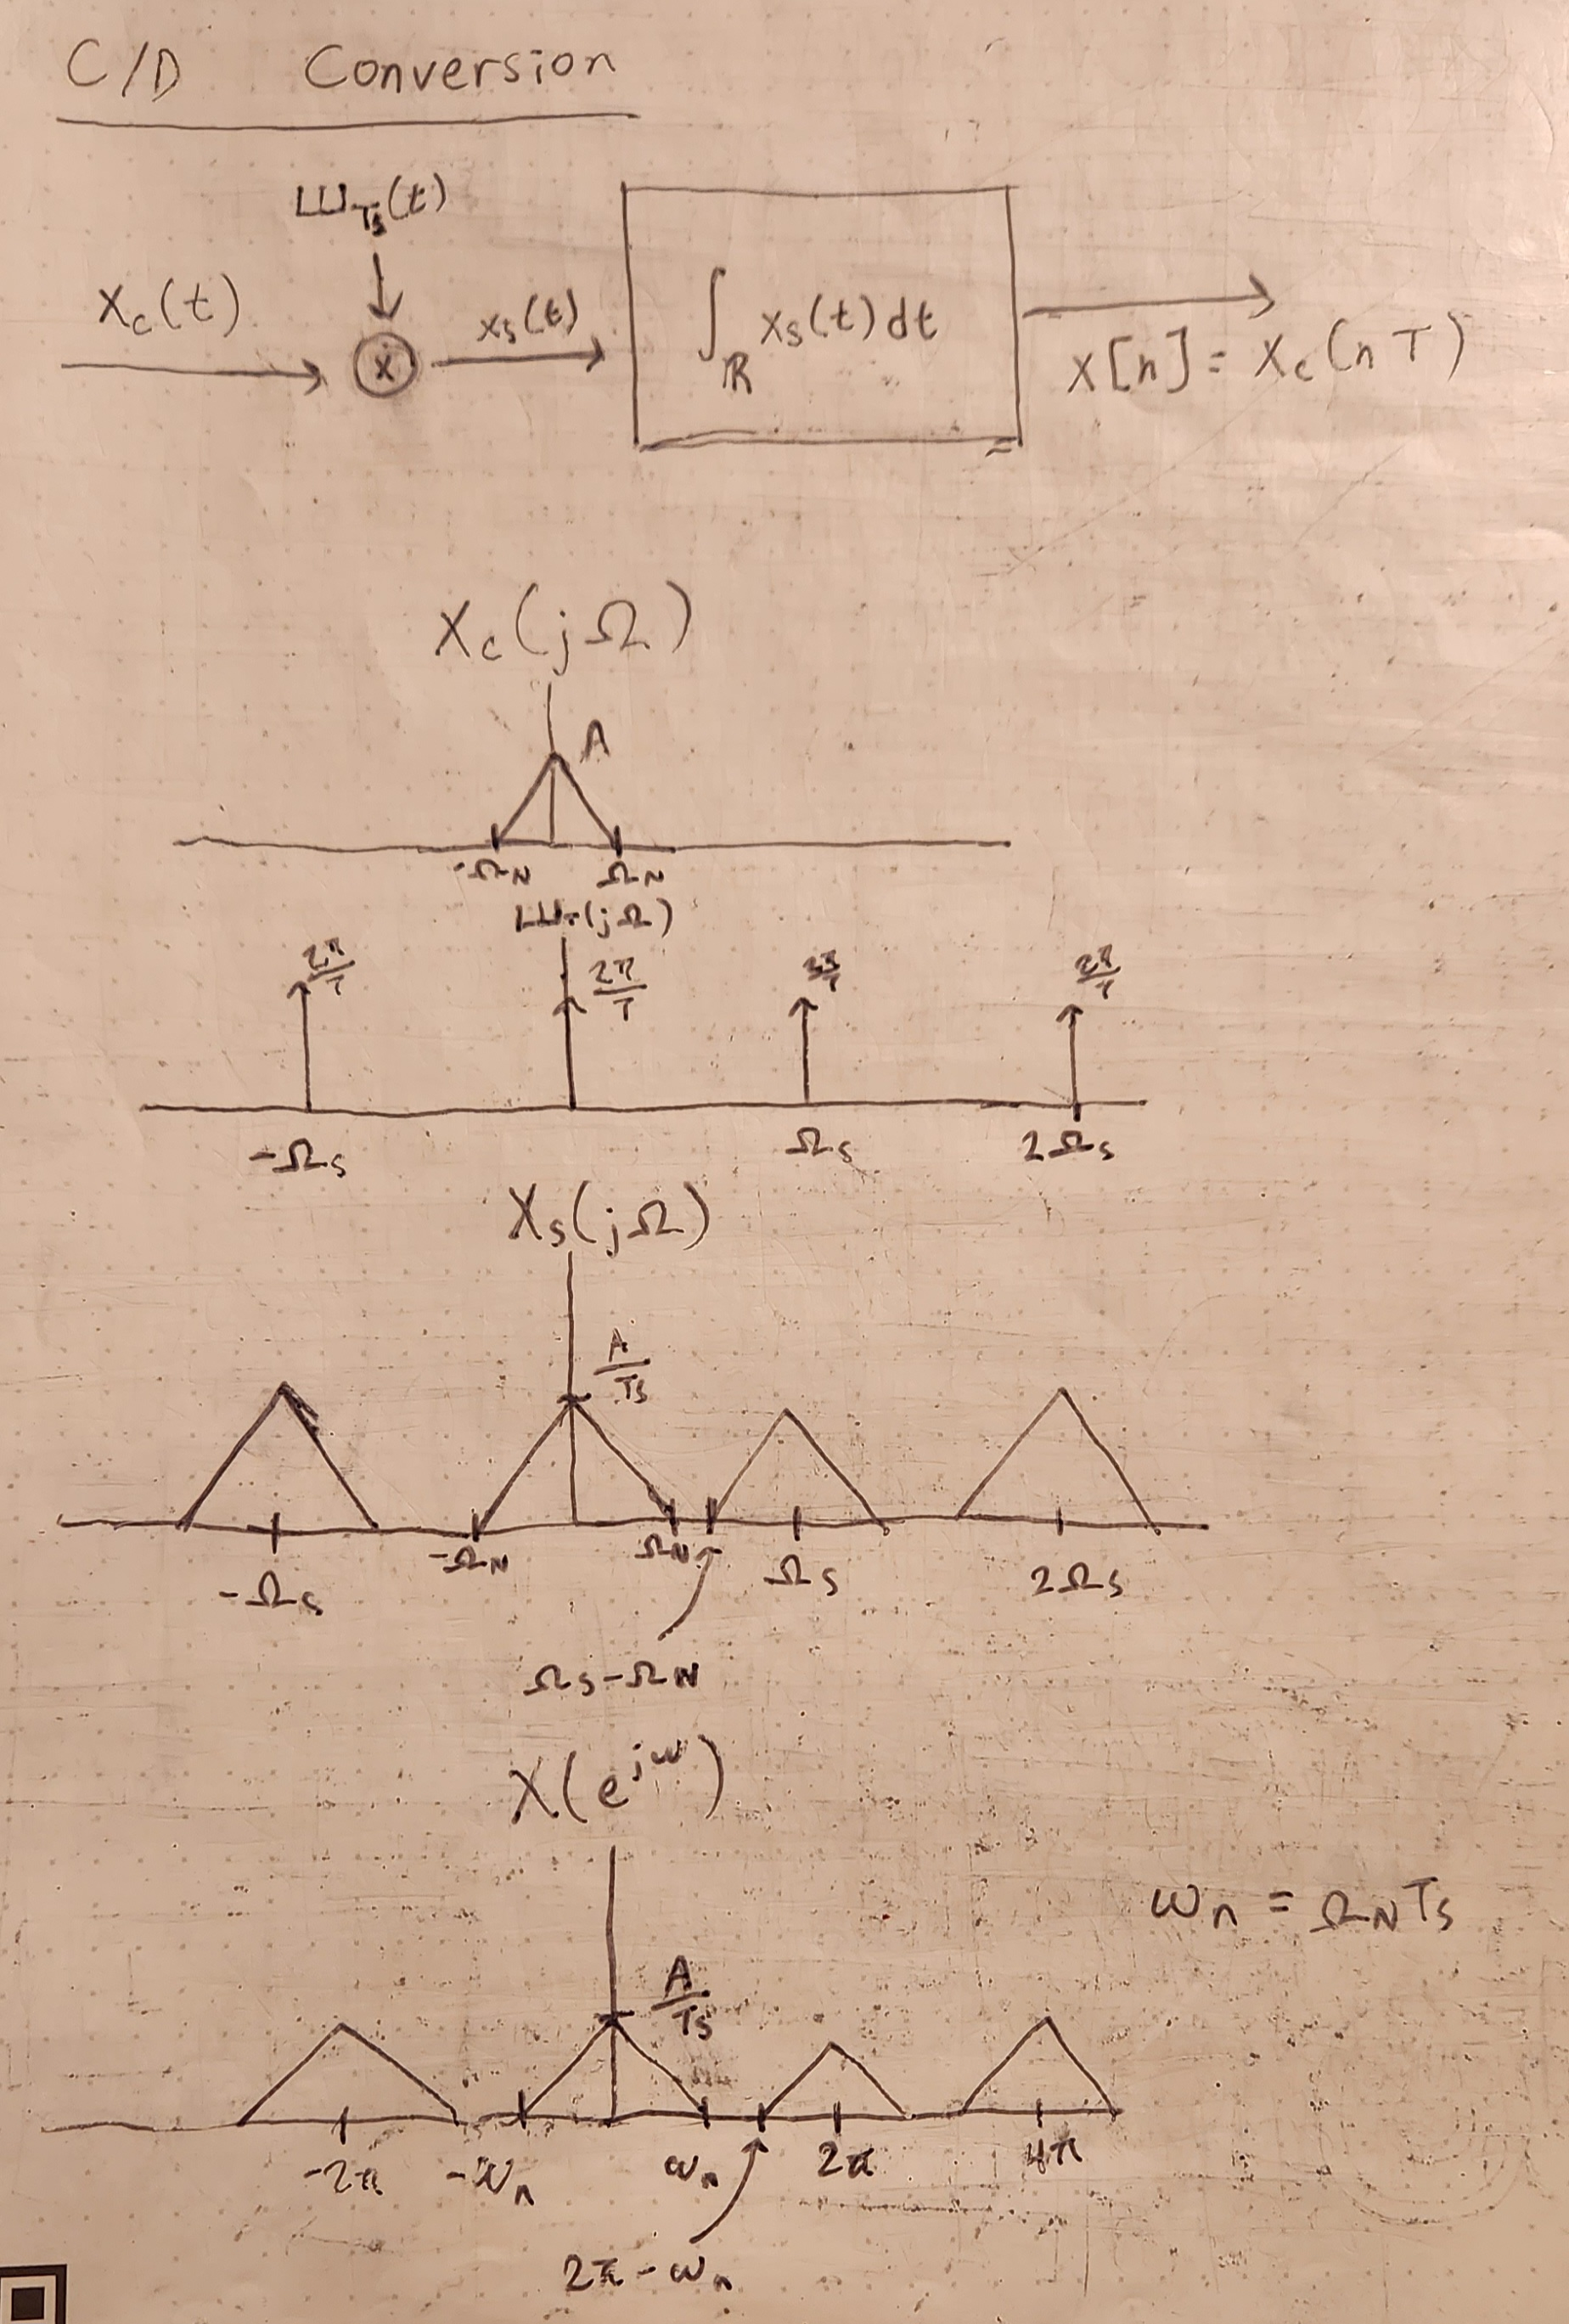
\includegraphics[scale=0.165]{graphics/cd_conversion.jpg}

  \pagebreak

  \subsubsection{D/C Conversion}

  \small\textbf{Mismatch in Reconstruction and Sampling Period}:

  Assuming no aliasing effects, if \(T_r \neq T_s\)

  \(y_r(t) = \dfrac{T_r}{T_s}x_c\prn{\dfrac{T_s}{T_r}t}\)

  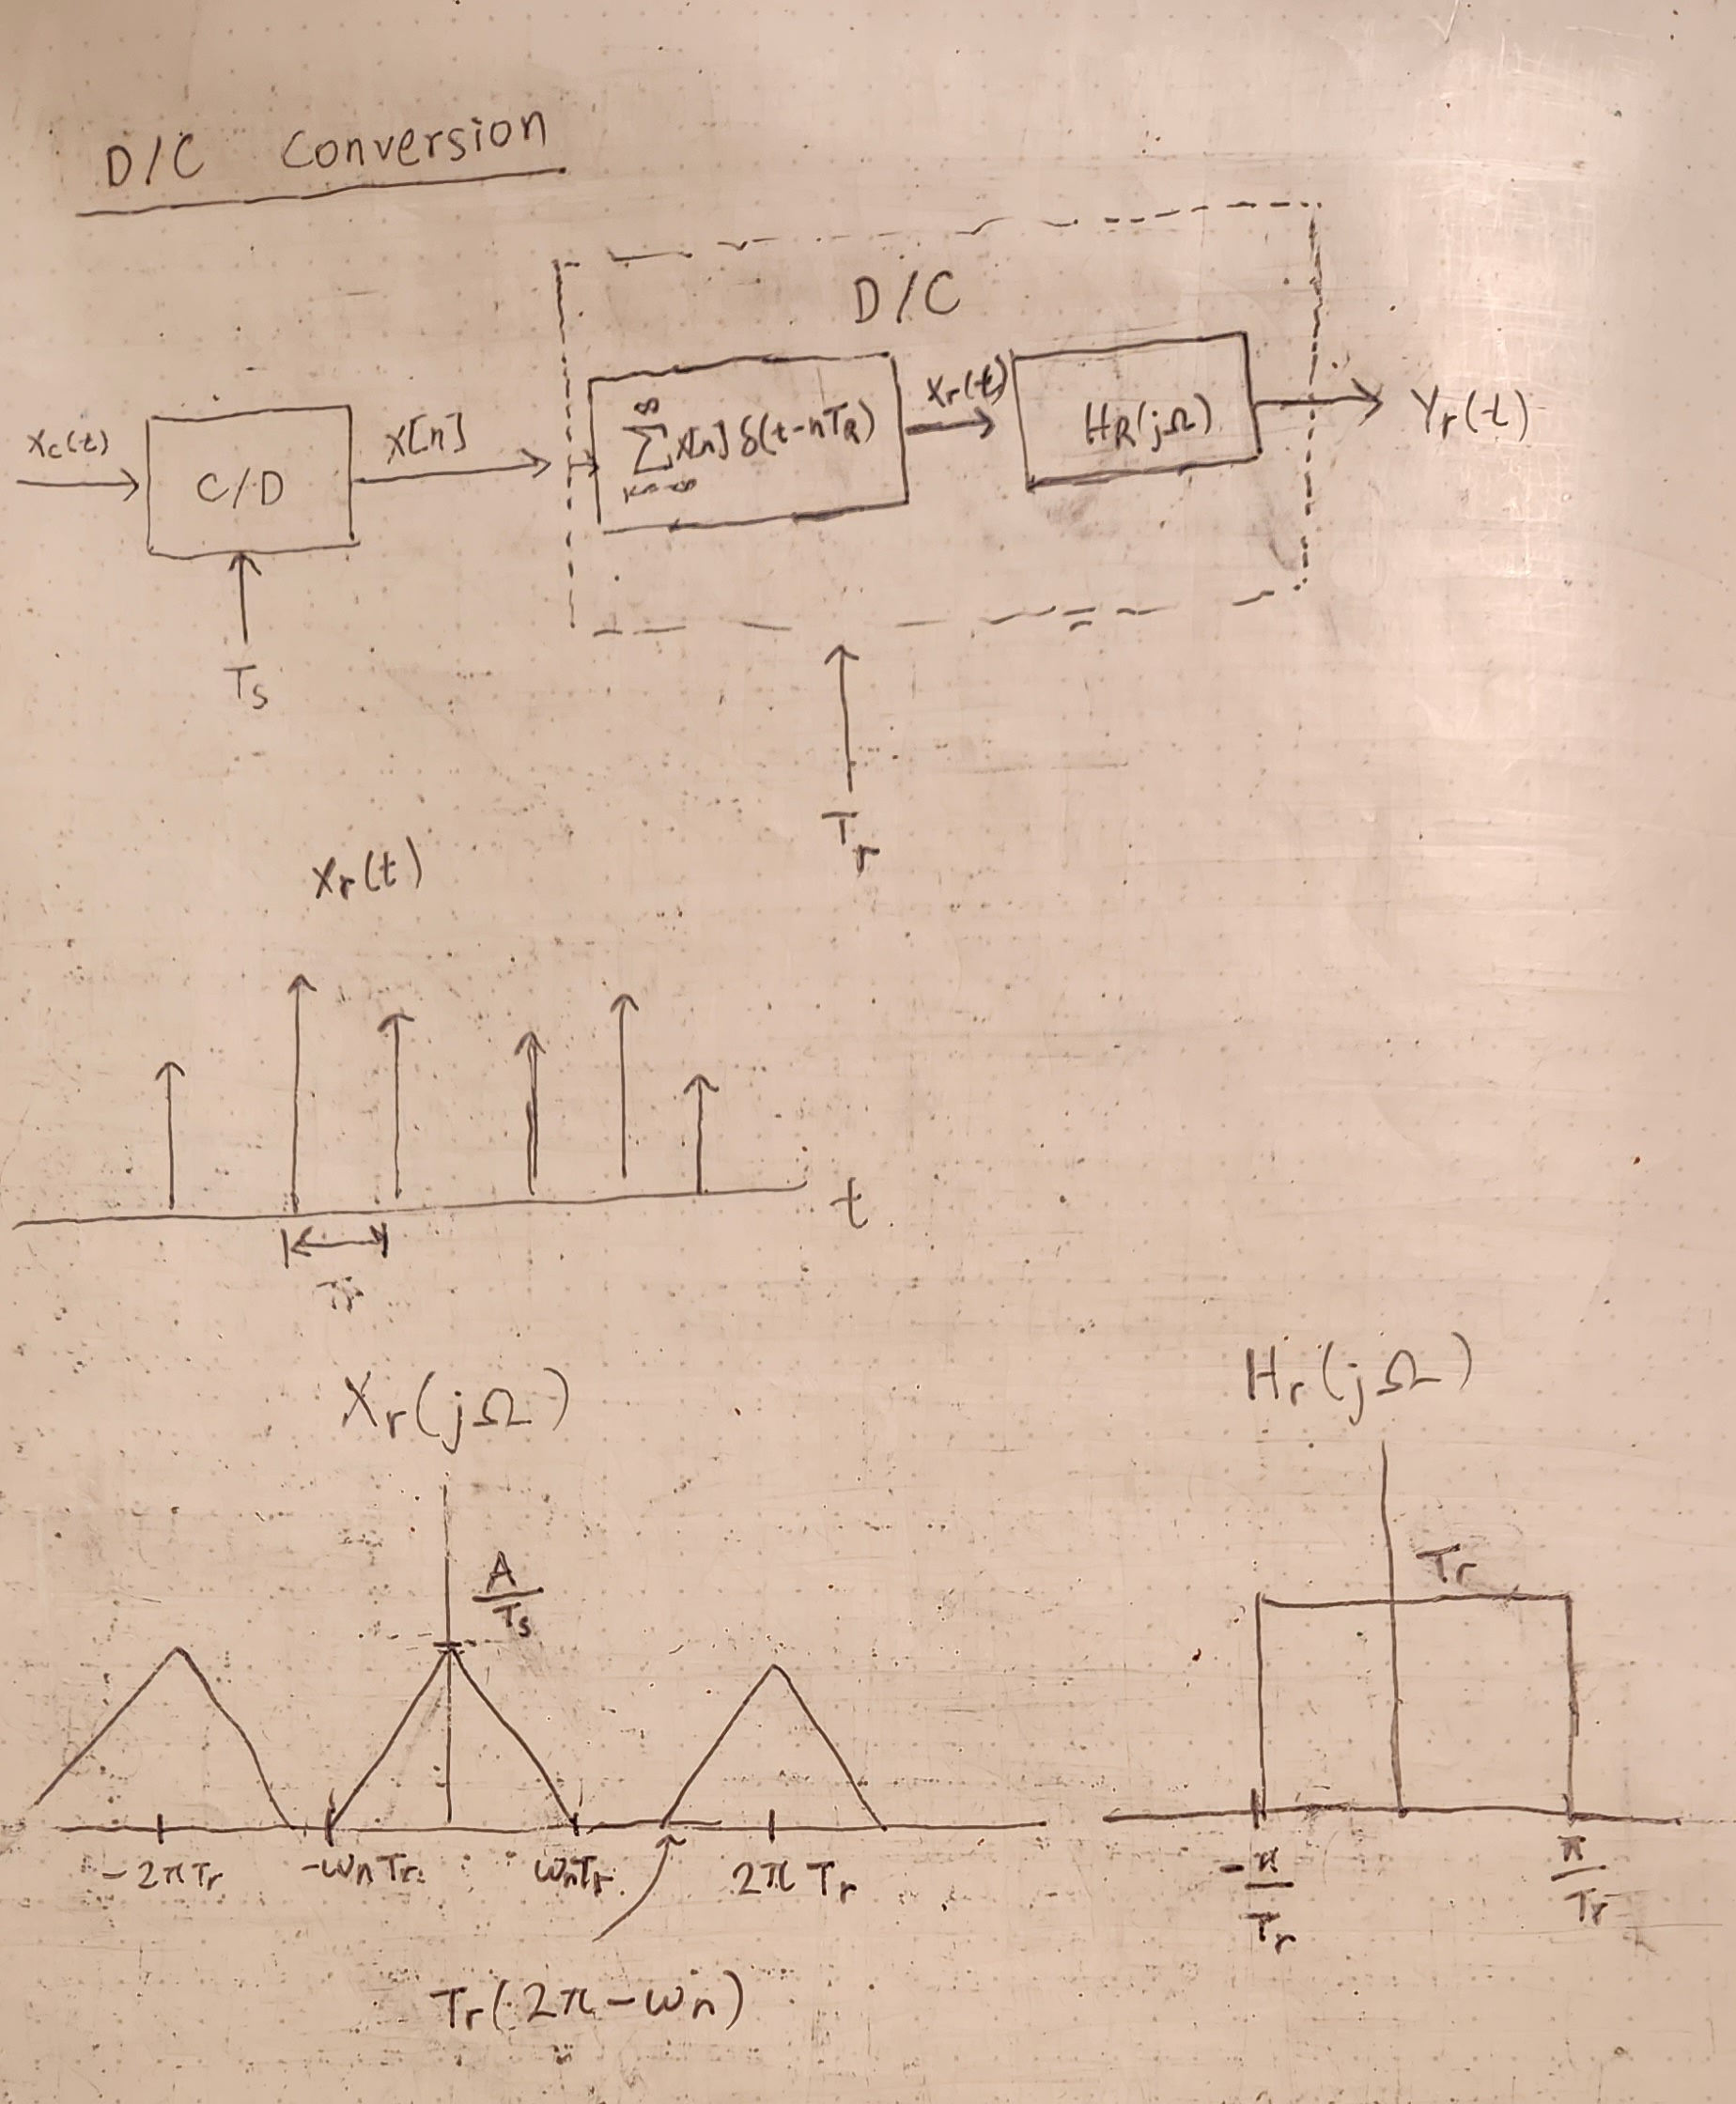
\includegraphics[scale=0.2]{graphics/dc_conversion.jpg}

  \pagebreak

  \subsubsection{Compression and Decimation}

  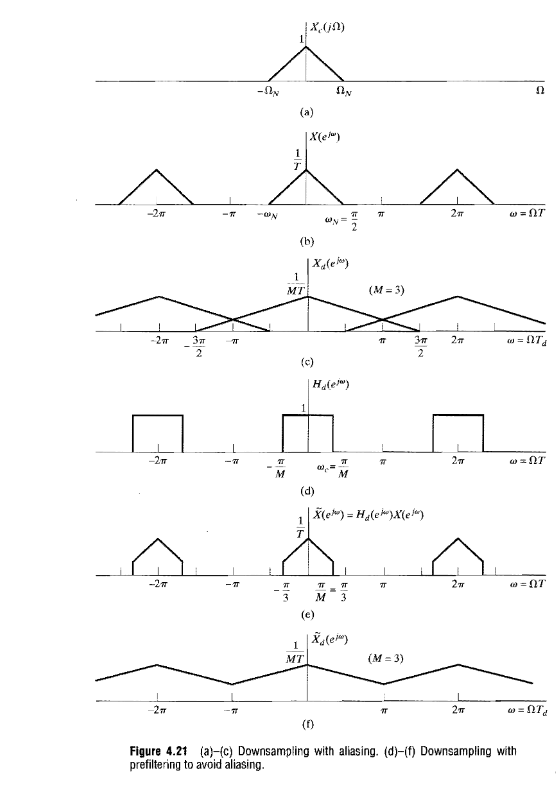
\includegraphics[scale=0.7]{graphics/downsampling.png}

  \pagebreak

  \subsubsection{Expansion and Interpolation}

  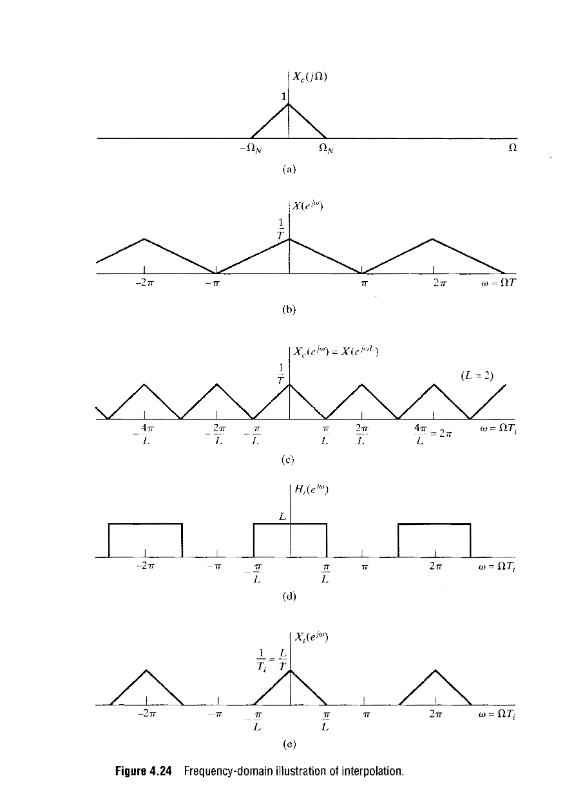
\includegraphics[scale=0.7]{graphics/upsampling.png}

  \pagebreak

  \subsubsection{Change Sampling Rate by Noninteger Factor}

  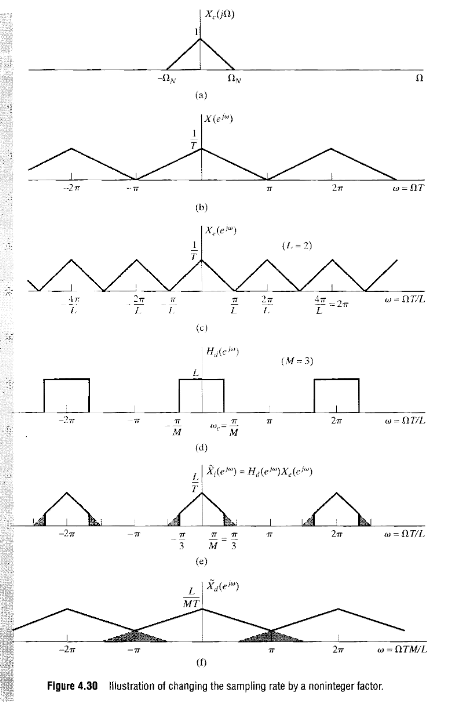
\includegraphics[scale=0.7]{graphics/noninteger.png}

  \pagebreak

  \subsubsection{Polyphase Decompositions}

  \textbf{Noble Identities:}

  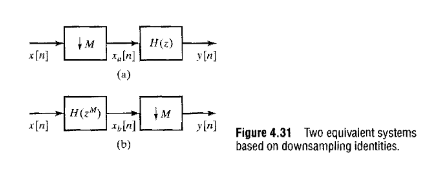
\includegraphics[scale=0.7]{graphics/compressor_noble.png}

  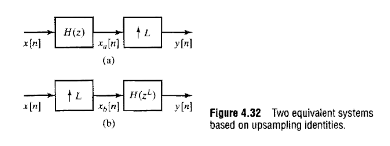
\includegraphics[scale=0.75]{graphics/expander_noble.png}

  \textbf{Polyphase Decomposition for Compression}:

  In the below diagram \(e_{k}[n] = h[nM + k]\)

  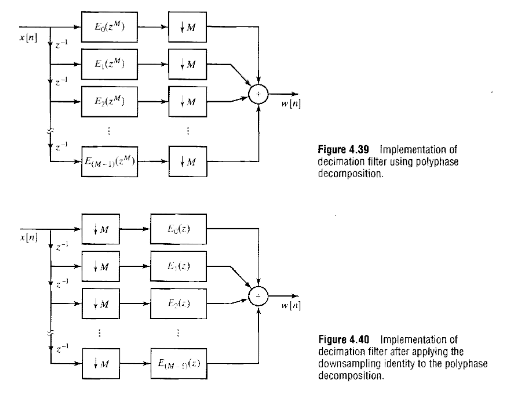
\includegraphics[scale=0.82]{graphics/polyphase_down.png}

\end{document}
